\documentclass[aspectratio=169]{beamer}

\usepackage{graphicx,hyperref,url}
\usepackage[english]{babel}
\usepackage[latin1]{inputenc}
%\usepackage{times}
\usepackage[T1]{fontenc}
\usepackage{multirow}
\usepackage{capt-of}
\usepackage{graphicx}
\usepackage{array}
\usepackage{tikz}
\usepackage{hyperref}
\usepackage{fes}

% Add a date and possibly the name of the event to the slides
%  - again first a short version to be shown at the bottom of each slide
%  - second the full date and event name for the title slide

\renewcommand{\(}{\begin{columns}}
\renewcommand{\)}{\end{columns}}
\newcommand{\<}[1]{\begin{column}{#1}}
\renewcommand{\>}{\end{column}}
%%%%%%%%%%%%%%%%%%%%%%%%%%%%%%%%%%%%%%%%%%%%%%%%%%



\newcommand{\degC}{$^o$C$\,$}
\newcommand{\co}{$\text{CO}_{2}\,$}

\newcommand{\coe}{$\text{CO}_{2}\text{e}\,$}
\newcommand{\tx}{$G_{2\times\text{CO}_2}$}
\newcommand{\Real}{\mathbb R}



\hypersetup{
    colorlinks=true,
    linkcolor=ualbertagold,
    filecolor=black,
    citecolor=black,
    urlcolor=ualbertagreen
}

% Optional: change font used by \url
\renewcommand{\UrlFont}{\normalfont}

% The main document



\begin{document}

\title[Carbon price pass-through]{Carbon price pass-through in Alberta's electricity market}

%\author{Branko Bo\v skovi\'{c} \and Andrew Leach \and Charles F.\ Mason}
%\institute{University of Alberta  \and University of Alberta  \and University of Wyoming}

%\author[shortname]{author1 \inst{1} \and author2 \inst{2}}
%\institute[shortinst]{\inst{1} affiliation for author1 \and %
 %                     \inst{2} affiliation for author2}



\author[Andrew Leach]{
\begin{columns}
      \column{.1\linewidth}
      \column{.8\linewidth}
      \vbox to .8\textheight{\centering
      Andrew Leach\\[1ex] Department of Economics (Arts) and Faculty of Law\\[1ex]University of Alberta
      }
      \vfill
      \column{.1\linewidth}
      \end{columns}
 }


\institute[QED]{
  Queeen's Economics Department\\
  Kingston, ON}


\date[QED Quant Seminar]{April, 2025}

\frame
  \titlepage
  
\section{Introduction}
\begin{frame}{Carbon Pricing's Effect on Electricity Markets}
    \begin{itemize}
    \item Research question: how do carbon pricing policy elements impact firm offer behaviour in electricity markets? 
    \item Electricity markets, at least in jurisdictions with competitive wholesale markets, are ideal environments in which to study responses to carbon prices
    \item A series of policy changes in Alberta altered carbon prices, output-based credit allocations, and coverage affecting different facilities differently over time
    \item Rich, hourly electricity market data allows for the identification of facility- and firm-level decisions with respect to carbon price pass-through
    \item Extensive emissions reporting data covering almost 20 years along with hourly weather across Alberta and daily commodity prices complete the data
        \end{itemize}
\vfill
\end{frame}

\begin{frame}{Results Preview}
    \begin{itemize}
    \item Limited (maximum of roughly 60\%) pass-through of carbon pricing costs in certain regions of the supply curve
    \item Physical constraints and market rules limit pass-through in lower-reaches of the hourly supply curve, leading to no pass-through in most cases
    \item Strategic incentives overwhelm carbon pricing pass-through in upper-reaches of the hourly supply curve, leading to limited pass-through
    \item Weak evidence of pass-through reaction to overall market tightness
    \item Caveat: offer choices are constrained at the upper and lower reaches of the merit order, and Tobit ML estimates not yet completed
        \end{itemize}
\vfill
\end{frame}

\section{Literature}

\begin{frame}{Literature on Carbon Price Pass-Through}
    \begin{itemize}
\item Fabra and Reguant (2014) finds pass-through of 110\% of costs in peak-hours and roughly 60\% in off-peak hours
\item Fabra and Reguant (2014) finds that lump-sum credit allocations were not distortionary in the short run
\item Hintermann (2016) finds pass-through rates of 81-111\% depending on the
hour of the day, and also finds that costs are fully passed-through on average. 
\item Kara et al. (2008) finds pass-through of 74\% in annual electricity prices in the Nordic area. 
\item Nazifi (2016) shows near-complete pass-through of Australian emissions prices to wholesale power prices
\item Jouvet and Solier (2013) finds insignificant pass-through in many hours in the EU.    
\item Brown et al. (2018) looks at the dynamics of the policies I study, but in a simplified, simulation model
\end{itemize}
\vfill
\end{frame}


\section{Motivation and Context}

%\begin{frame}{Oil sands reserves\hspace{3cm} \small Source: AER (2013)}
%\pgfputat{\pgfxy(0,.25)}{\pgfimage[width=4.25in]{AB_reserves.pdf}}
%\end{frame}

\begin{frame}{Why Alberta? Other than the obvious...}
    \begin{itemize}
    \item Alberta's power market is relatively small, isolated, and features a mix of generation technologies
    \item Transparent wholesale market offer process, and significant hourly variability in intertie capacity and renewable generation, helps with identification
\item Substantial variation in policies: three provincial regulatory regimes (2007, 2018, 2020) and one federal regime (2018) with increases in prices in many years (2016, 2017, 2020-2025)   
\item Policies varied in prices, coverage, and the formulae governing the issuance of output-based allocations as well
\item Provincial and federal emissions reporting and compliance data are public
\item A personal connection to many of the policies, in particular Alberta's \emph{CCIR} implemented in 2018 and the federal carbon pricing regime
  \end{itemize}
\vfill
\end{frame}

\section{Alberta Markets and Policies}

\begin{frame}{How does Alberta's Wholesale Power Market Work?}
   \tikz [remember picture,overlay]
    \node[yshift=-0.7cm,xshift=0cm] at (current page.center)
        {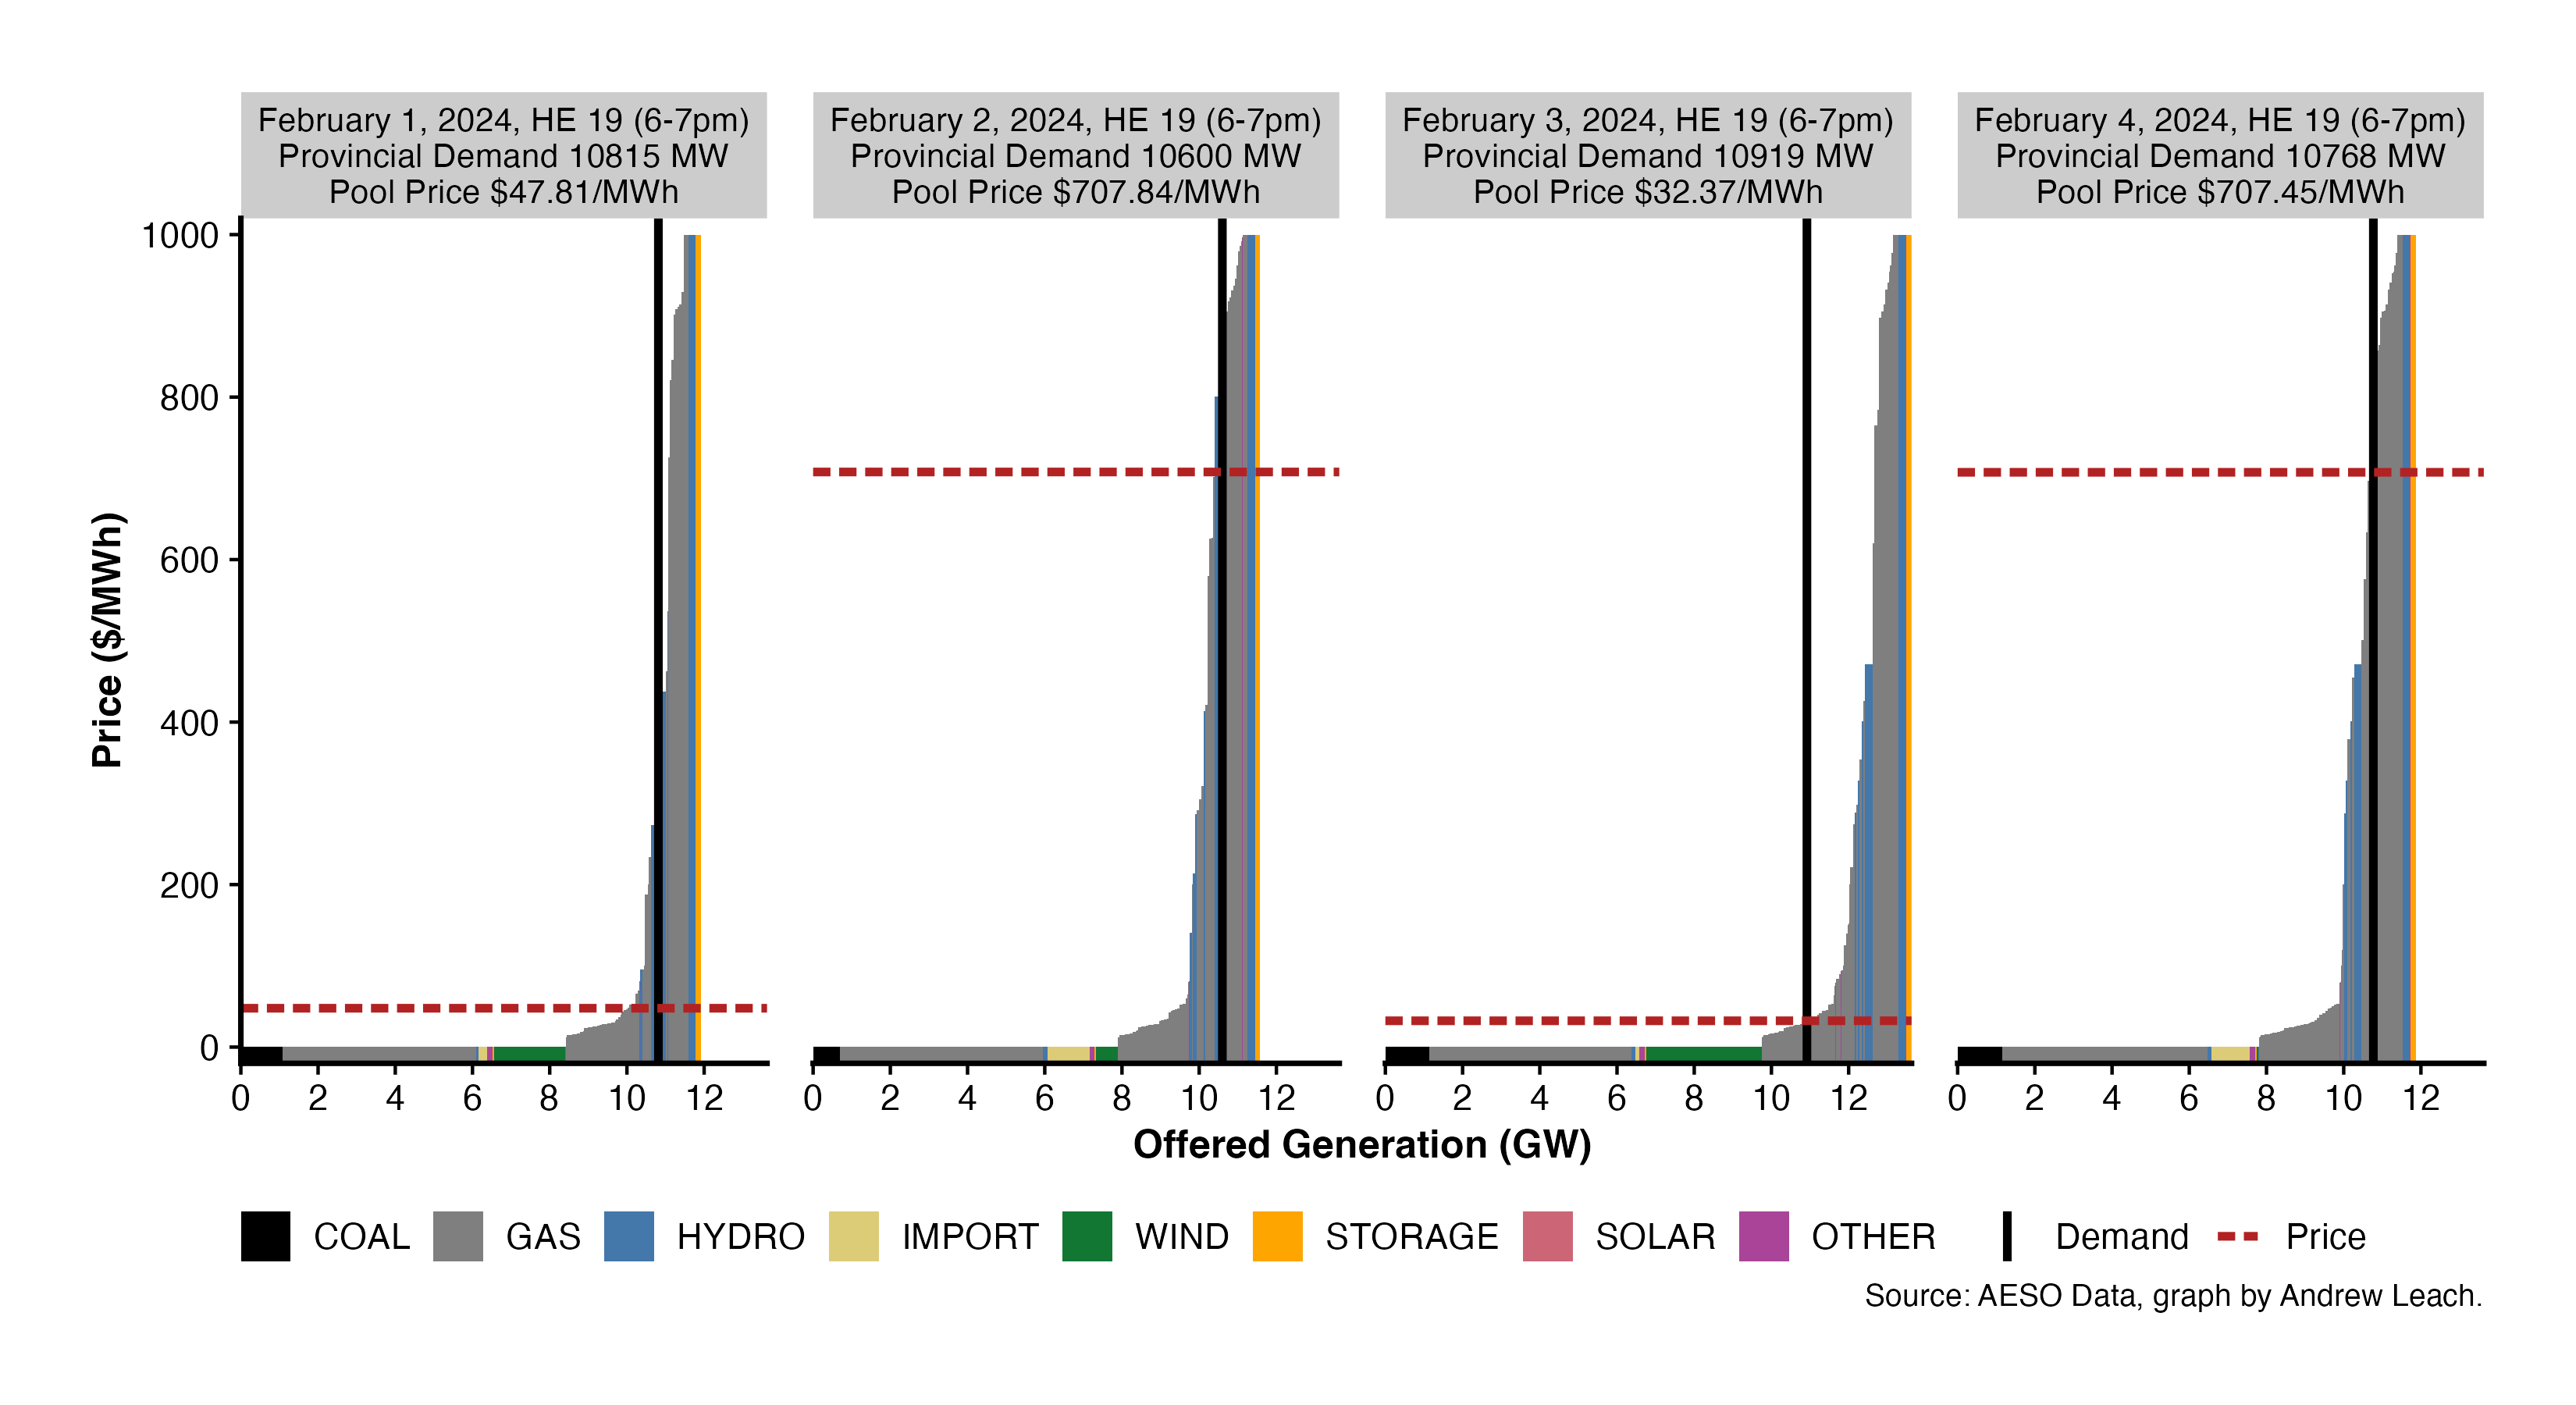
\includegraphics[width=.9\paperwidth]{../images/merit_examples.png}}; \vspace{1cm}
   \vfill
\end{frame}


\begin{frame}{Price Volatility}
   \tikz [remember picture,overlay]
    \node[yshift=0cm,xshift=0cm] at (current page.center)
        {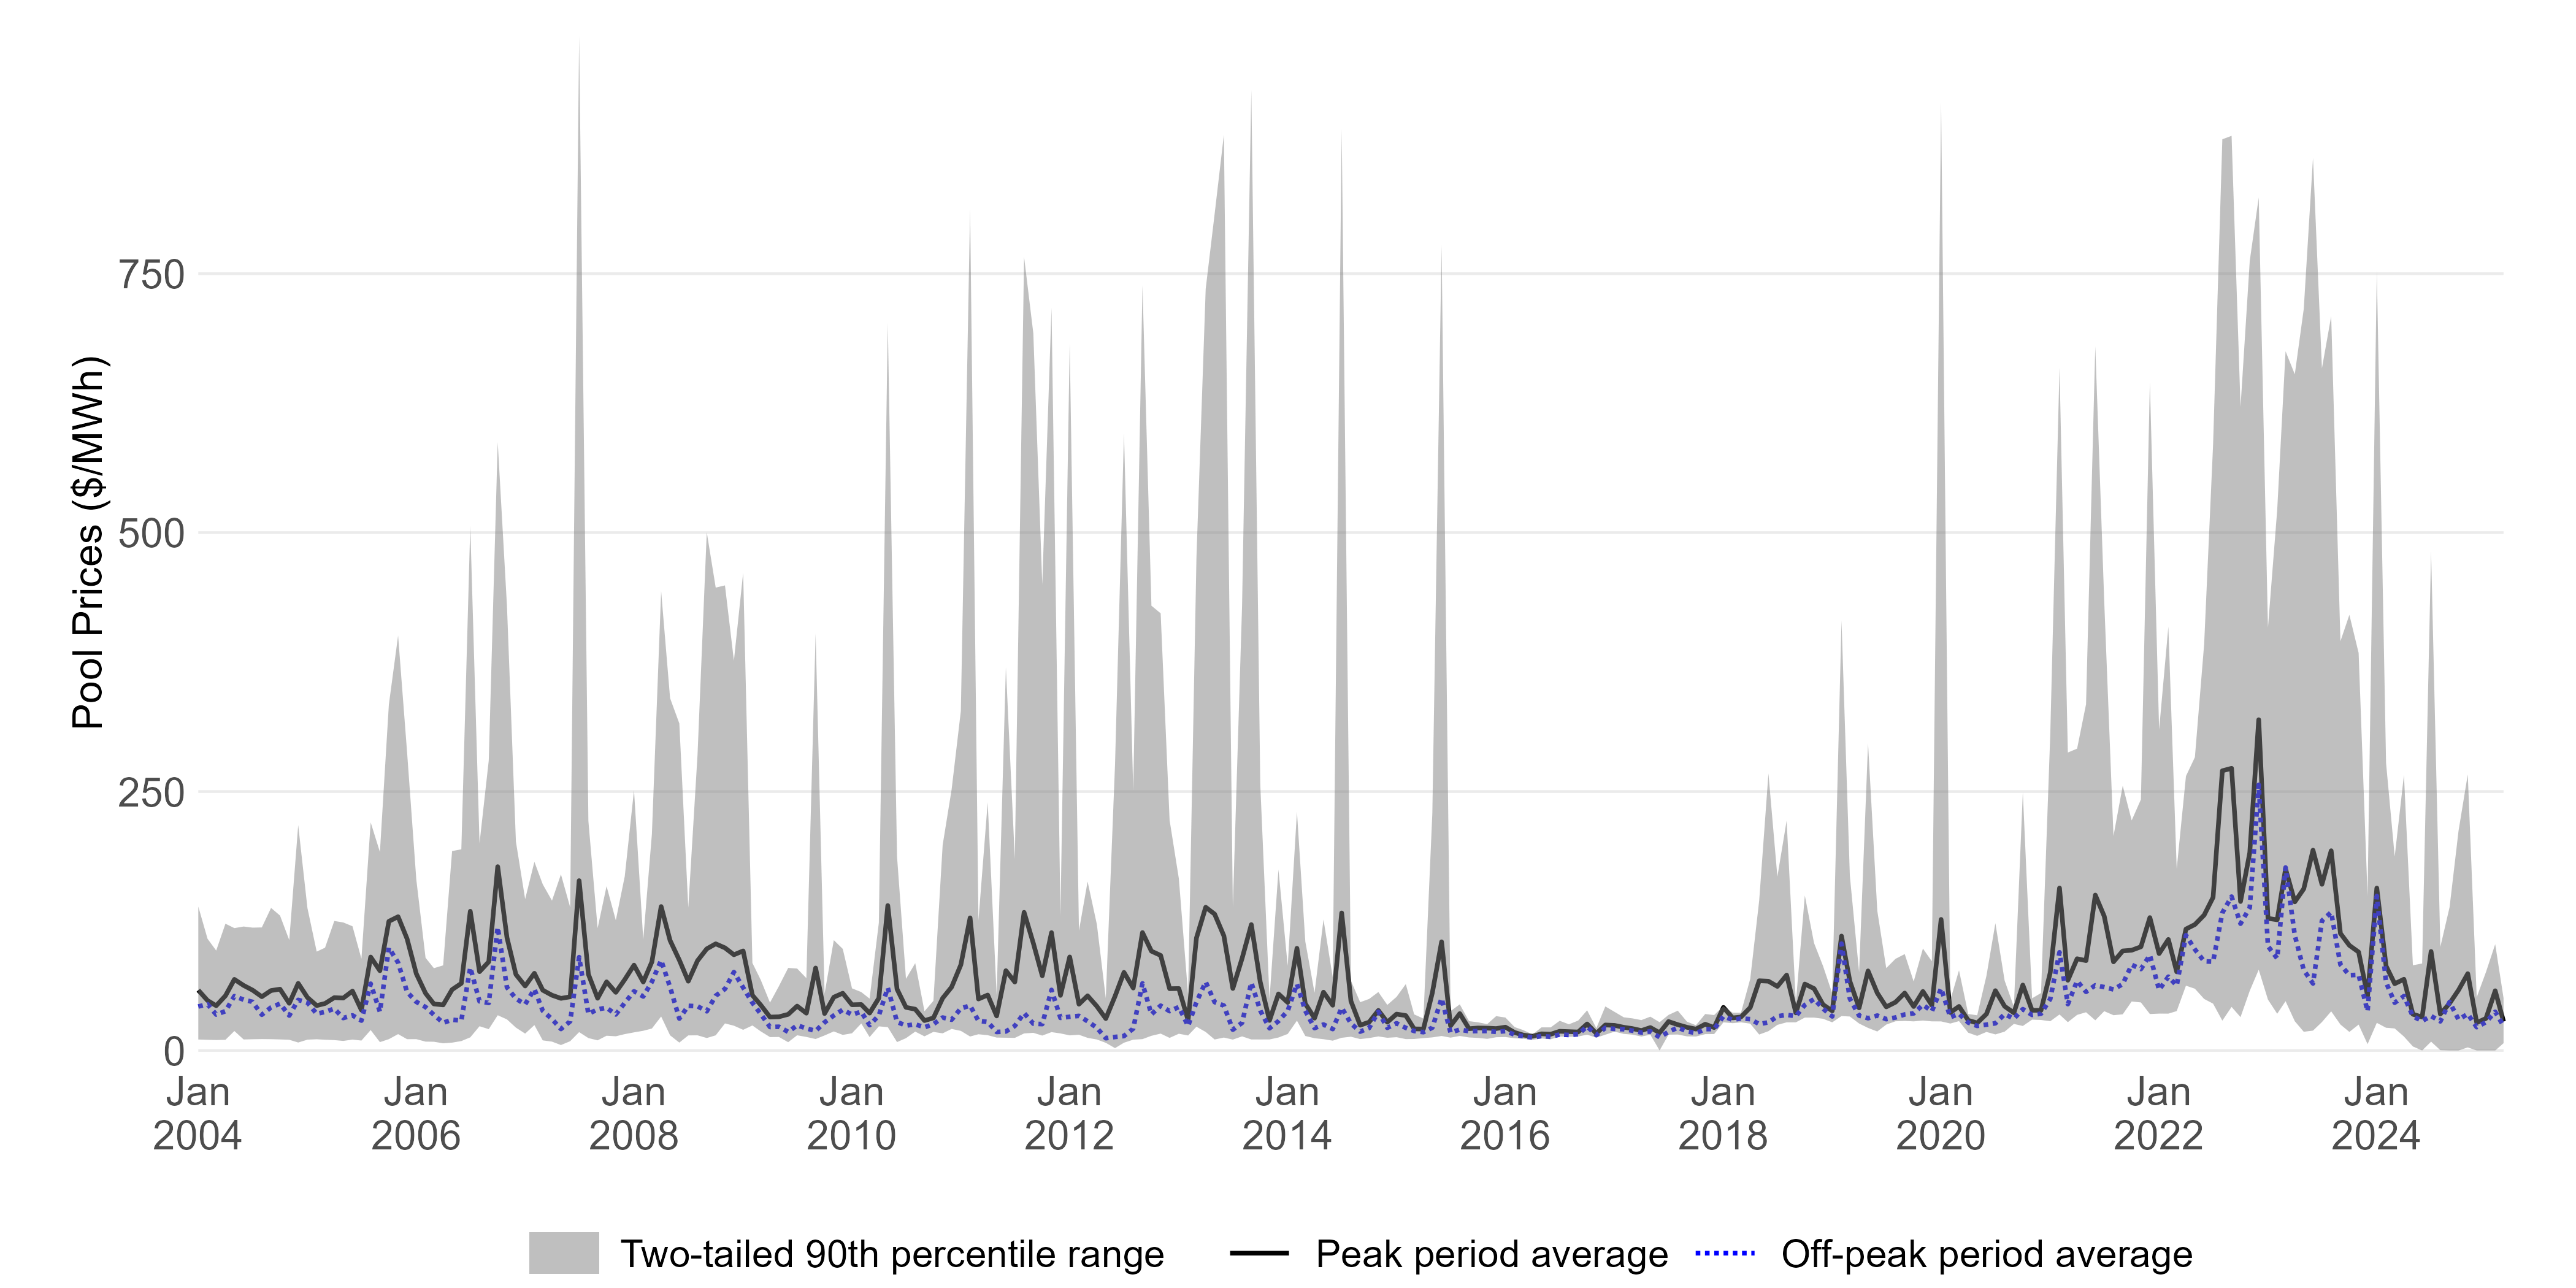
\includegraphics[width=.92\paperwidth]{../images/peak_prices.png}};   \vfill
\end{frame}


\begin{frame}
   \tikz [remember picture,overlay]
    \node[yshift=-0.2cm,xshift=0cm] at (current page.center)
        {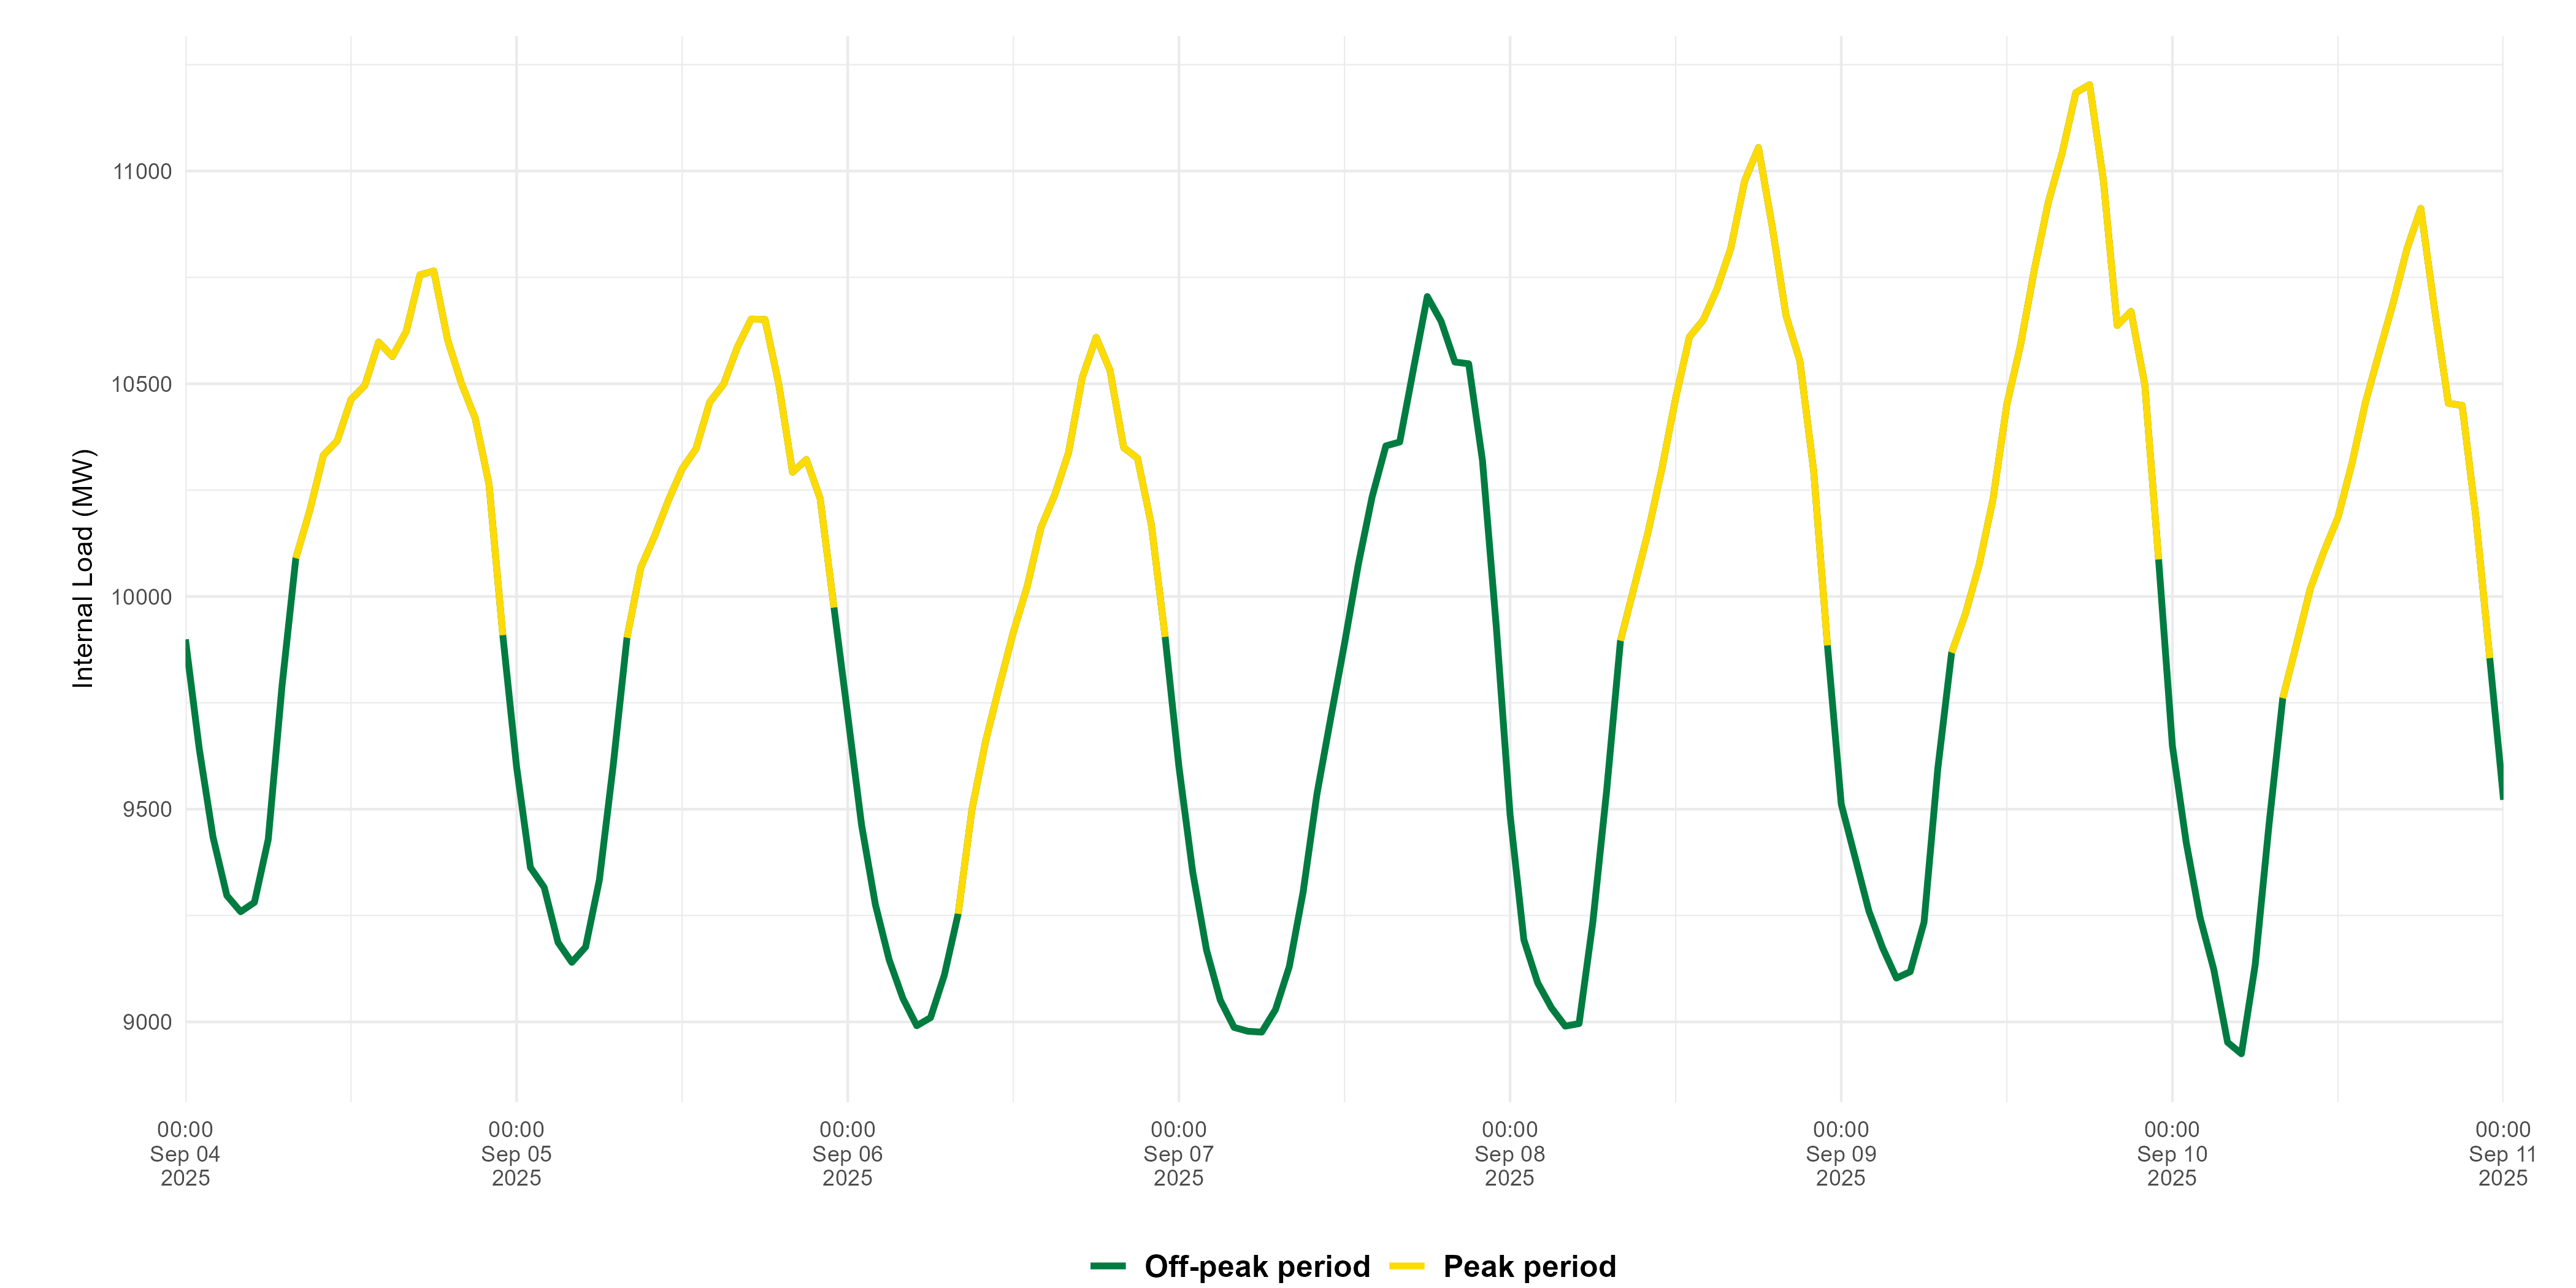
\includegraphics[width=.92\paperwidth]{../images/loads_clean.png}}; \vspace{1cm}
   \vfill
\end{frame}



\begin{frame}{Alberta GHG Emissions Policies}
    \begin{itemize}
    \item \emph{SGER} 1.0 (2007-2015): carbon price of \$15/t\coe, OBA at 88\% of historic emissions intensity, coverage for facilities with emissions above 100,000t\coe/yr
\item \emph{SGER} 2.0 (2016-2017): carbon price increased to \$20/t\coe for 2017 and to \$30/t\coe for 2018, while OBA rates decline to 85\% of historic emissions intensity for 2017 and 80\% for 2018
\item \emph{CCIR} (2018-2019): carbon price remains at \$30/t\coe but OBA rates set to 0.37t/MWh for most participants. Coverage remains at 100,000 tonnes per year.
\item Alberta Carbon Tax (2018-2019): carbon price set at \$30/t\coe expanded to cover facilities not covered by \emph{CCIR}, with opt-in available
\item \emph{TIER} (2020-present): carbon price follows federal schedule (\$30/t\coe in 2020 $\rightarrow$ \$95/t\coe today), with coverage and OBA same as \emph{CCIR} for electricity sector.
\item Federal carbon tax (2020-2024): carbon price follows federal schedule (\$30/t\coe in 2020 $\rightarrow$ \$95/t\coe today), applies to entities not covered by \emph{TIER}

  \end{itemize}
\vfill
\end{frame}



\begin{frame}{Variation in Compliance Costs}
   \tikz [remember picture,overlay]
    \node[yshift=-0.5cm,xshift=0cm] at (current page.center)
        {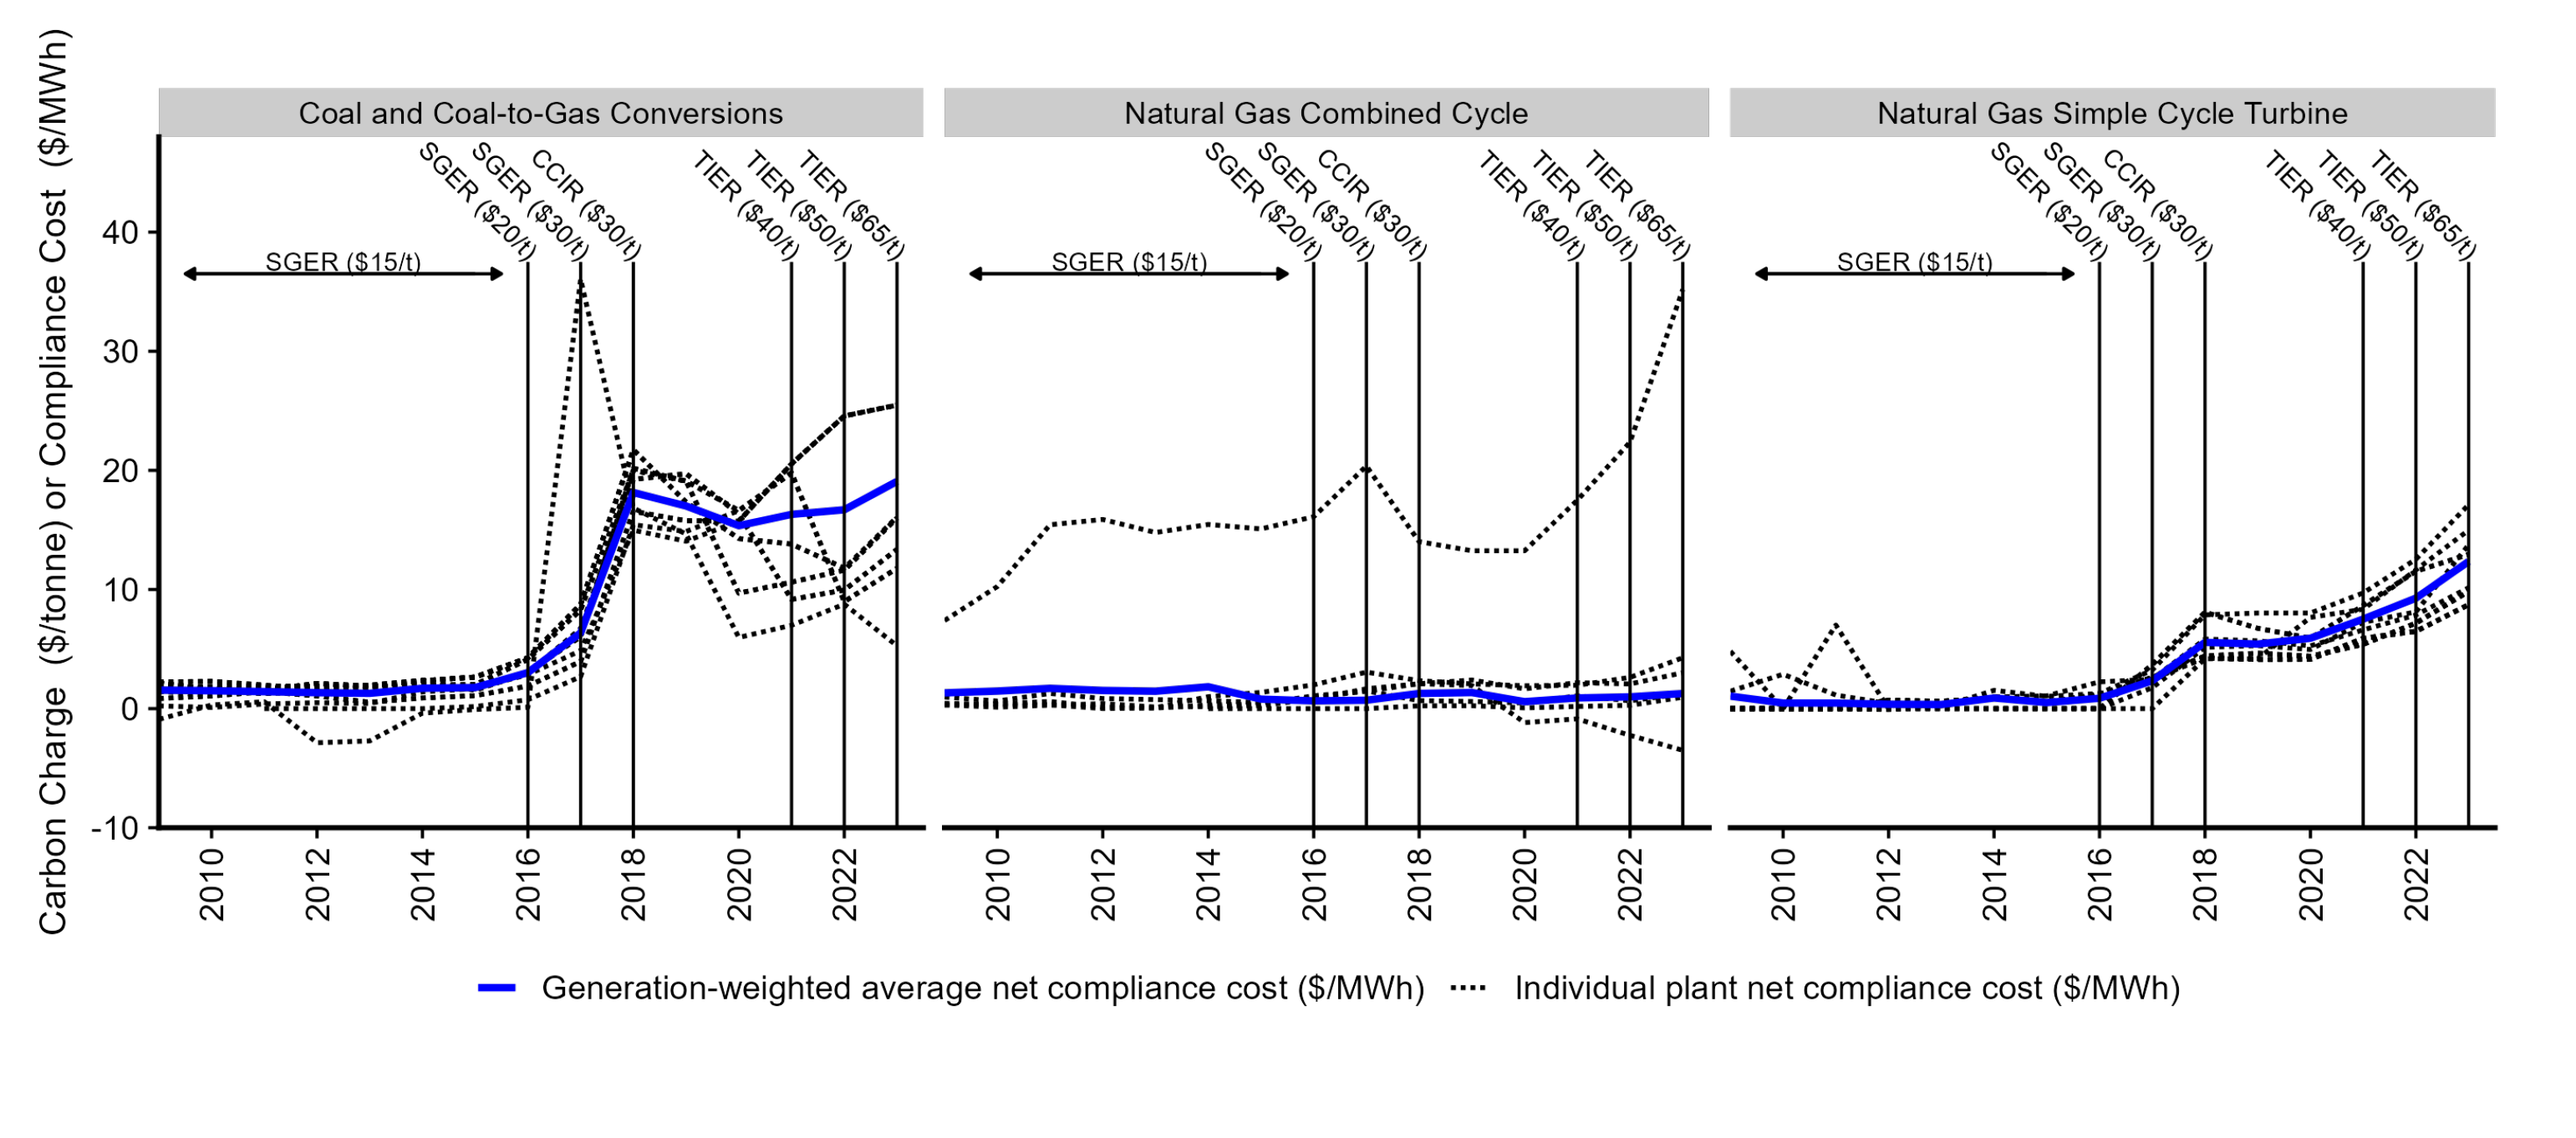
\includegraphics[width=.9\paperwidth]{compliance.png}}; \vspace{1cm}
   \vfill
\end{frame}



\begin{frame}
   \tikz [remember picture,overlay]
    \node[yshift=-0.2cm,xshift=0cm] at (current page.center)
        {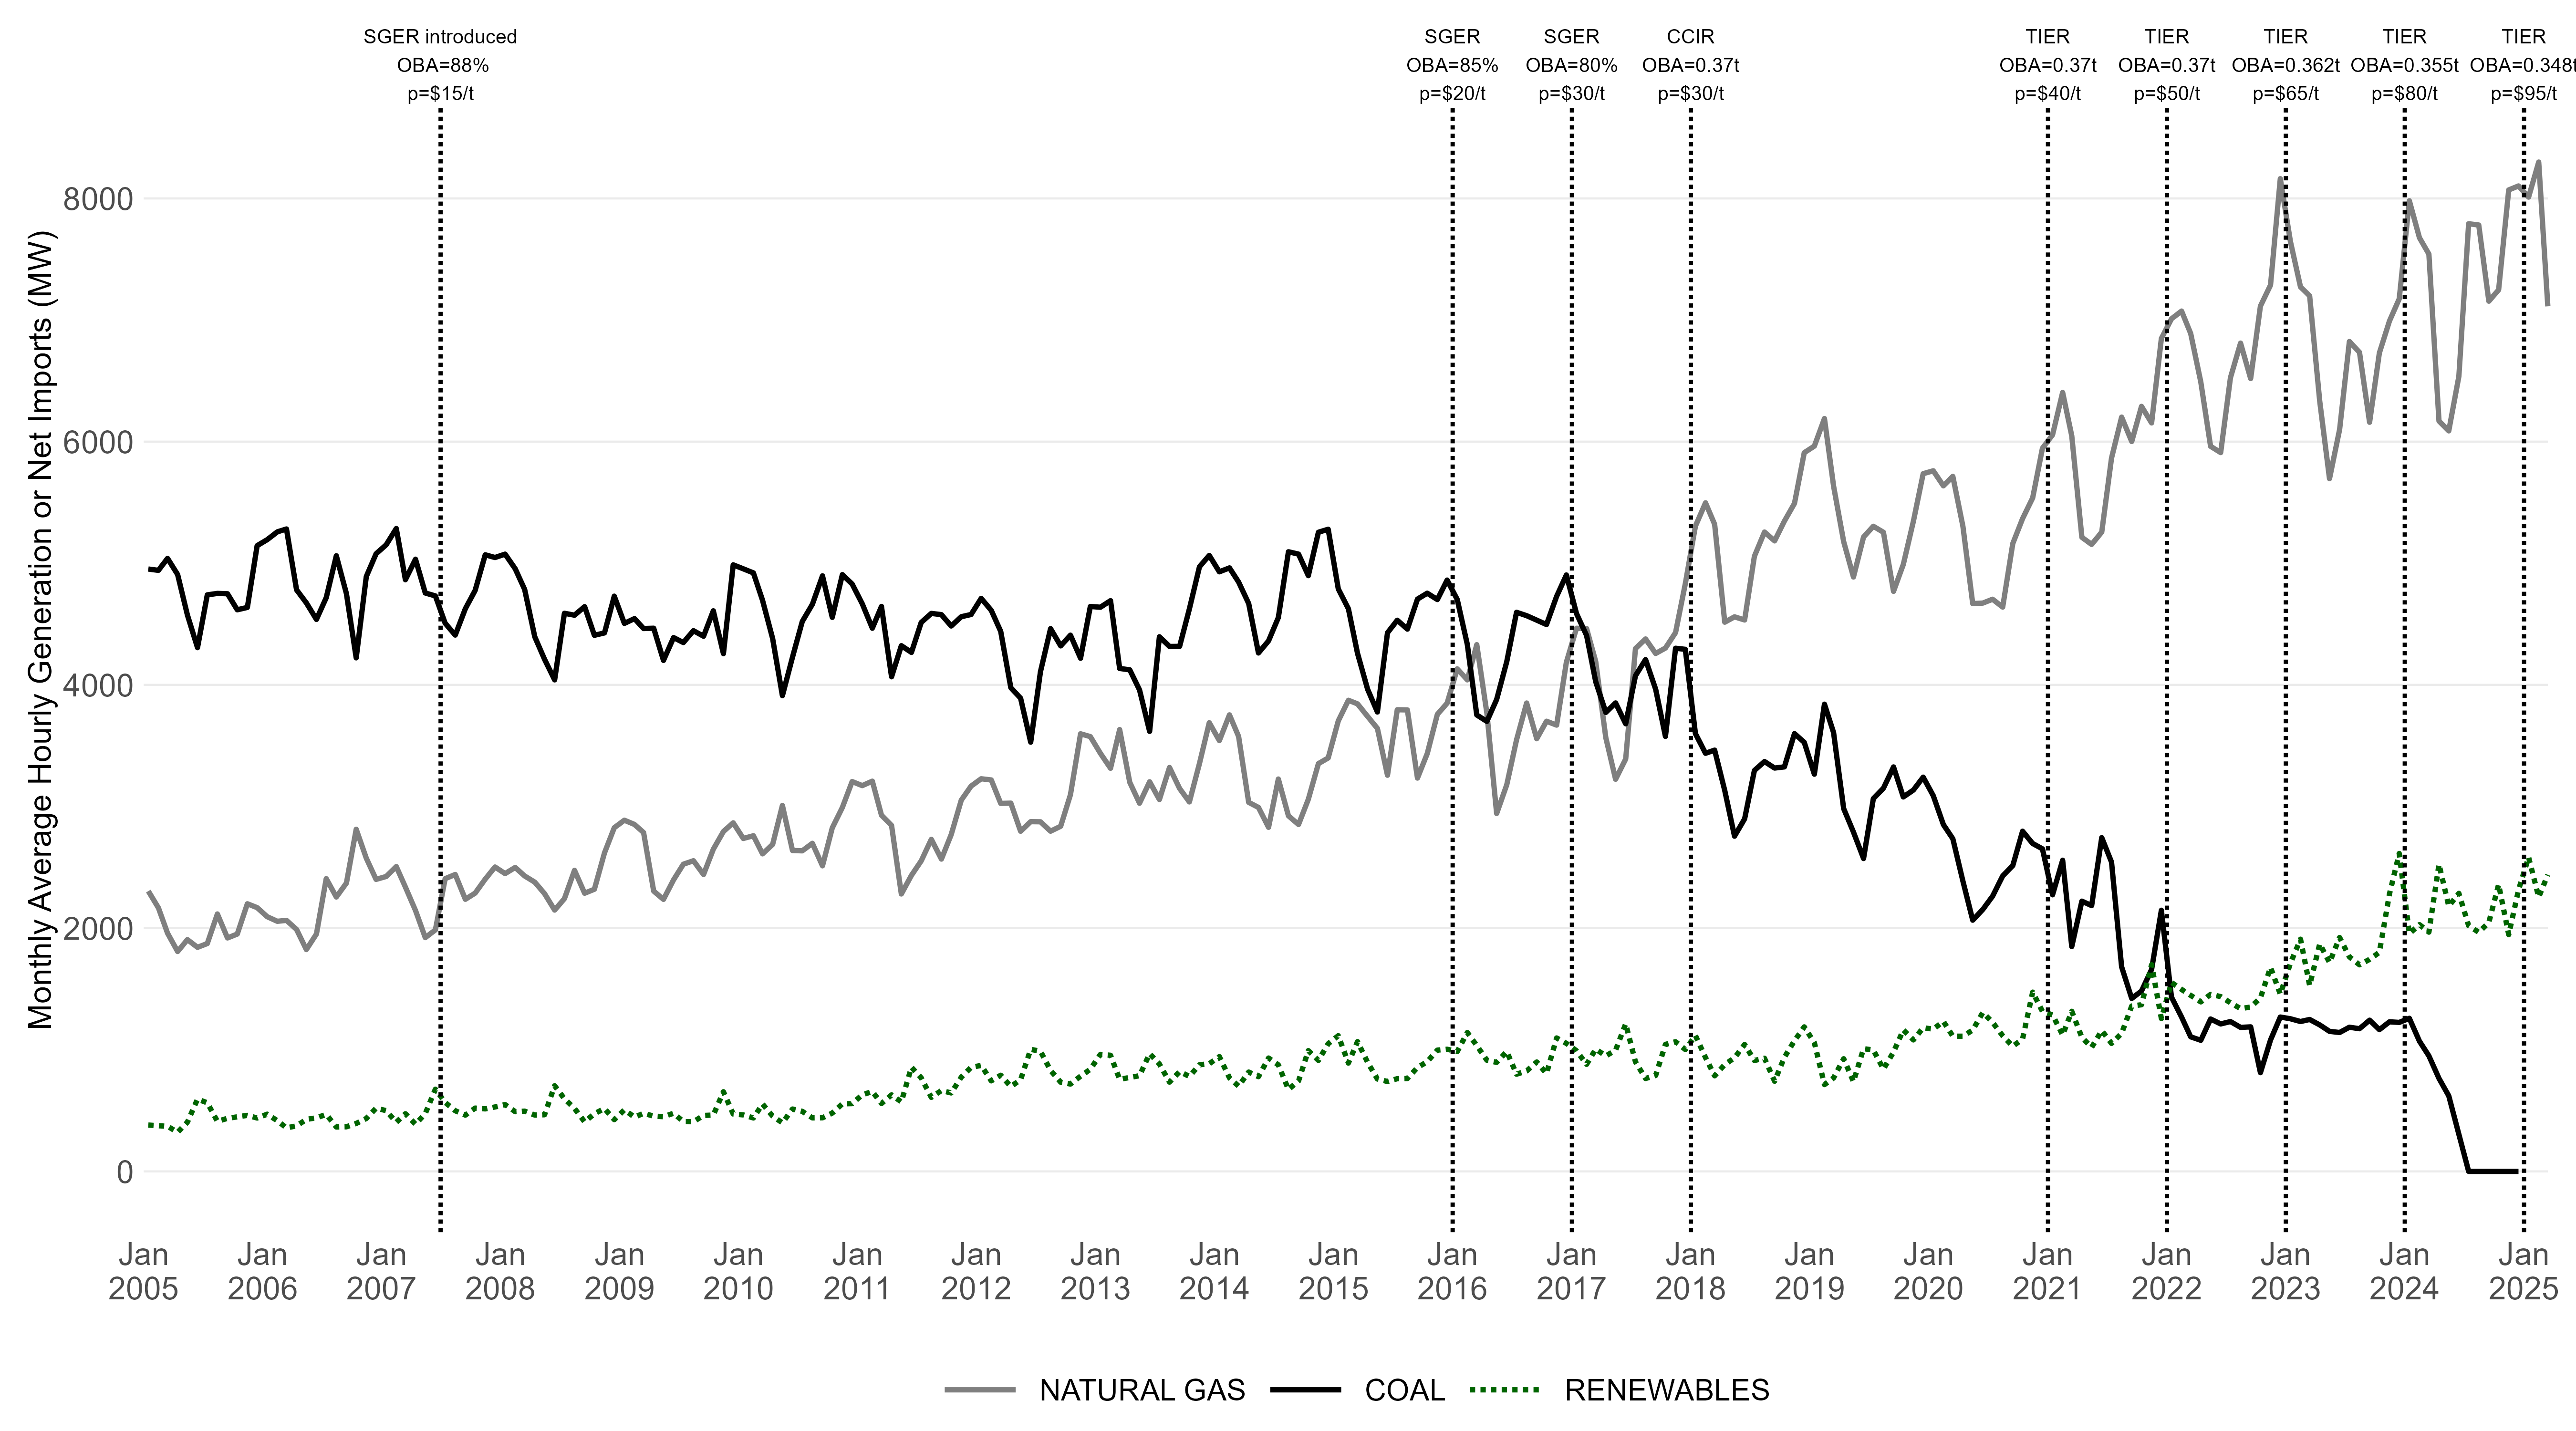
\includegraphics[width=.9\paperwidth]{../images/gen_fuel_policies.png}}; \vspace{1cm}
   \vfill
\end{frame}



\begin{frame}{Market Power in Alberta's Electricity System}
    \begin{itemize}
    \item Electricity generation was restructured in the 1990s and early 2000s
    \item Market was highly concentrated with legacy, regulated utility generators
    \item Power Purchase Arrangements (PPAs) introduced as an alternative to divestiture to mitigate market power in generation
    \item PPA change in law clause triggered with respect to the changes in \emph{SGER} 2.0 and all PPAs returned to government entity (the Balancing Pool)
    \item Balancing Pool becomes dominant player in the market until PPAs expire at the end of 2020
    \item Alberta market becomes much more concentrated again, particularly among dispatchable units
    \item New generation construction has (had?) mitigated market power to some degree, although an acquisition in 2024-25 has the potential to return the market to a highly-concentrated state

  \end{itemize}
\vfill
\end{frame}



\begin{frame}
   \tikz [remember picture,overlay]
    \node[yshift=-0.3cm,xshift=0cm] at (current page.center)
        {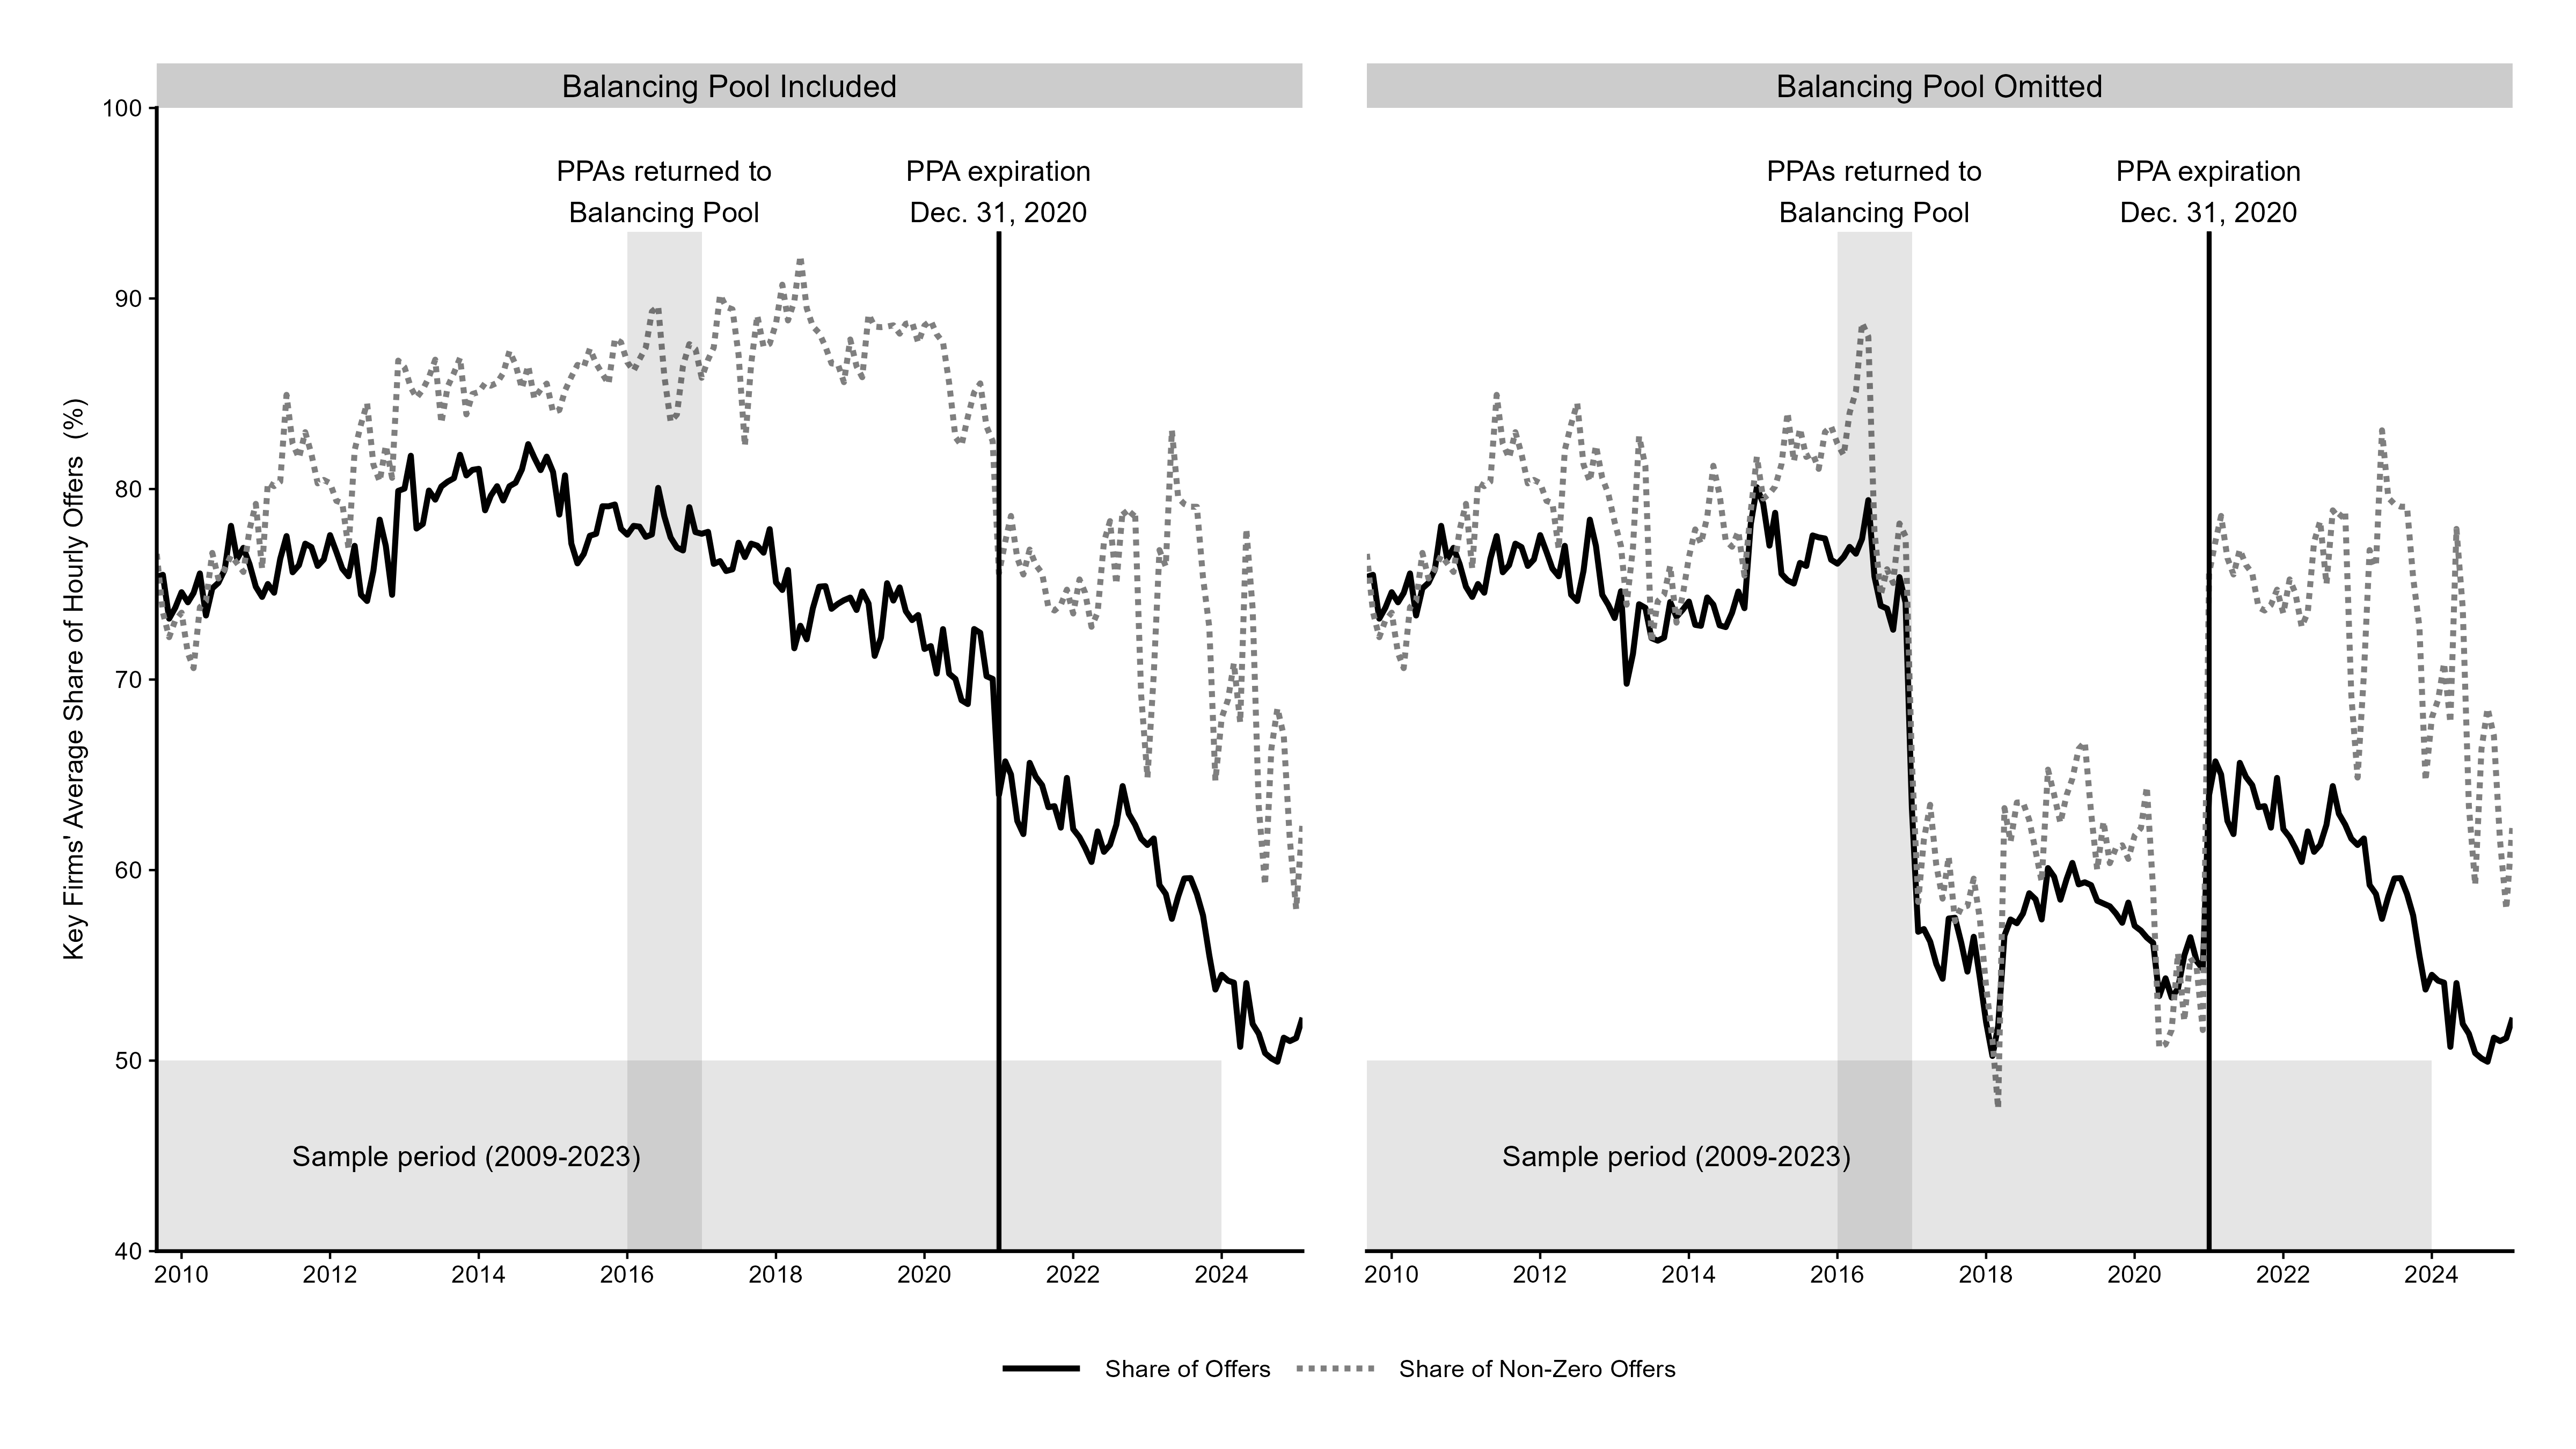
\includegraphics[width=.92\paperwidth]{../images/mkt_power.png}}; \vspace{1cm}
   \vfill
\end{frame}



\section{Data}

\begin{frame}{Data set is comprised of 27.7 million observations linking:}
    \begin{itemize}
    \item Hourly facility-level offers (up to 7 increasing-price blocks per facility, 2009-2025)
    \item Block-level offer control (only 2013-2025)
    \item Annual emissions-intensity by facility (2004-2023)
    \item Hourly electricity market conditions including renewable generation, trade, intertie capability, load, price, market concentration, etc. (2003-2025)
    \item Hourly weather in three regions of Alberta (2003-2025)
    \item Daily commodity price (natural gas) data (2003-2025)
    \item Facility characteristics (fuel, capacity, etc. 2003-2025)
    \item Annual emissions policy parameters including carbon prices and output-based allocations (2003-2025)
  \end{itemize}
\vfill
\end{frame}


\begin{frame}{Recall the Merit Order}
   \tikz [remember picture,overlay]
    \node[yshift=-0.5cm,xshift=0cm] at (current page.center)
        {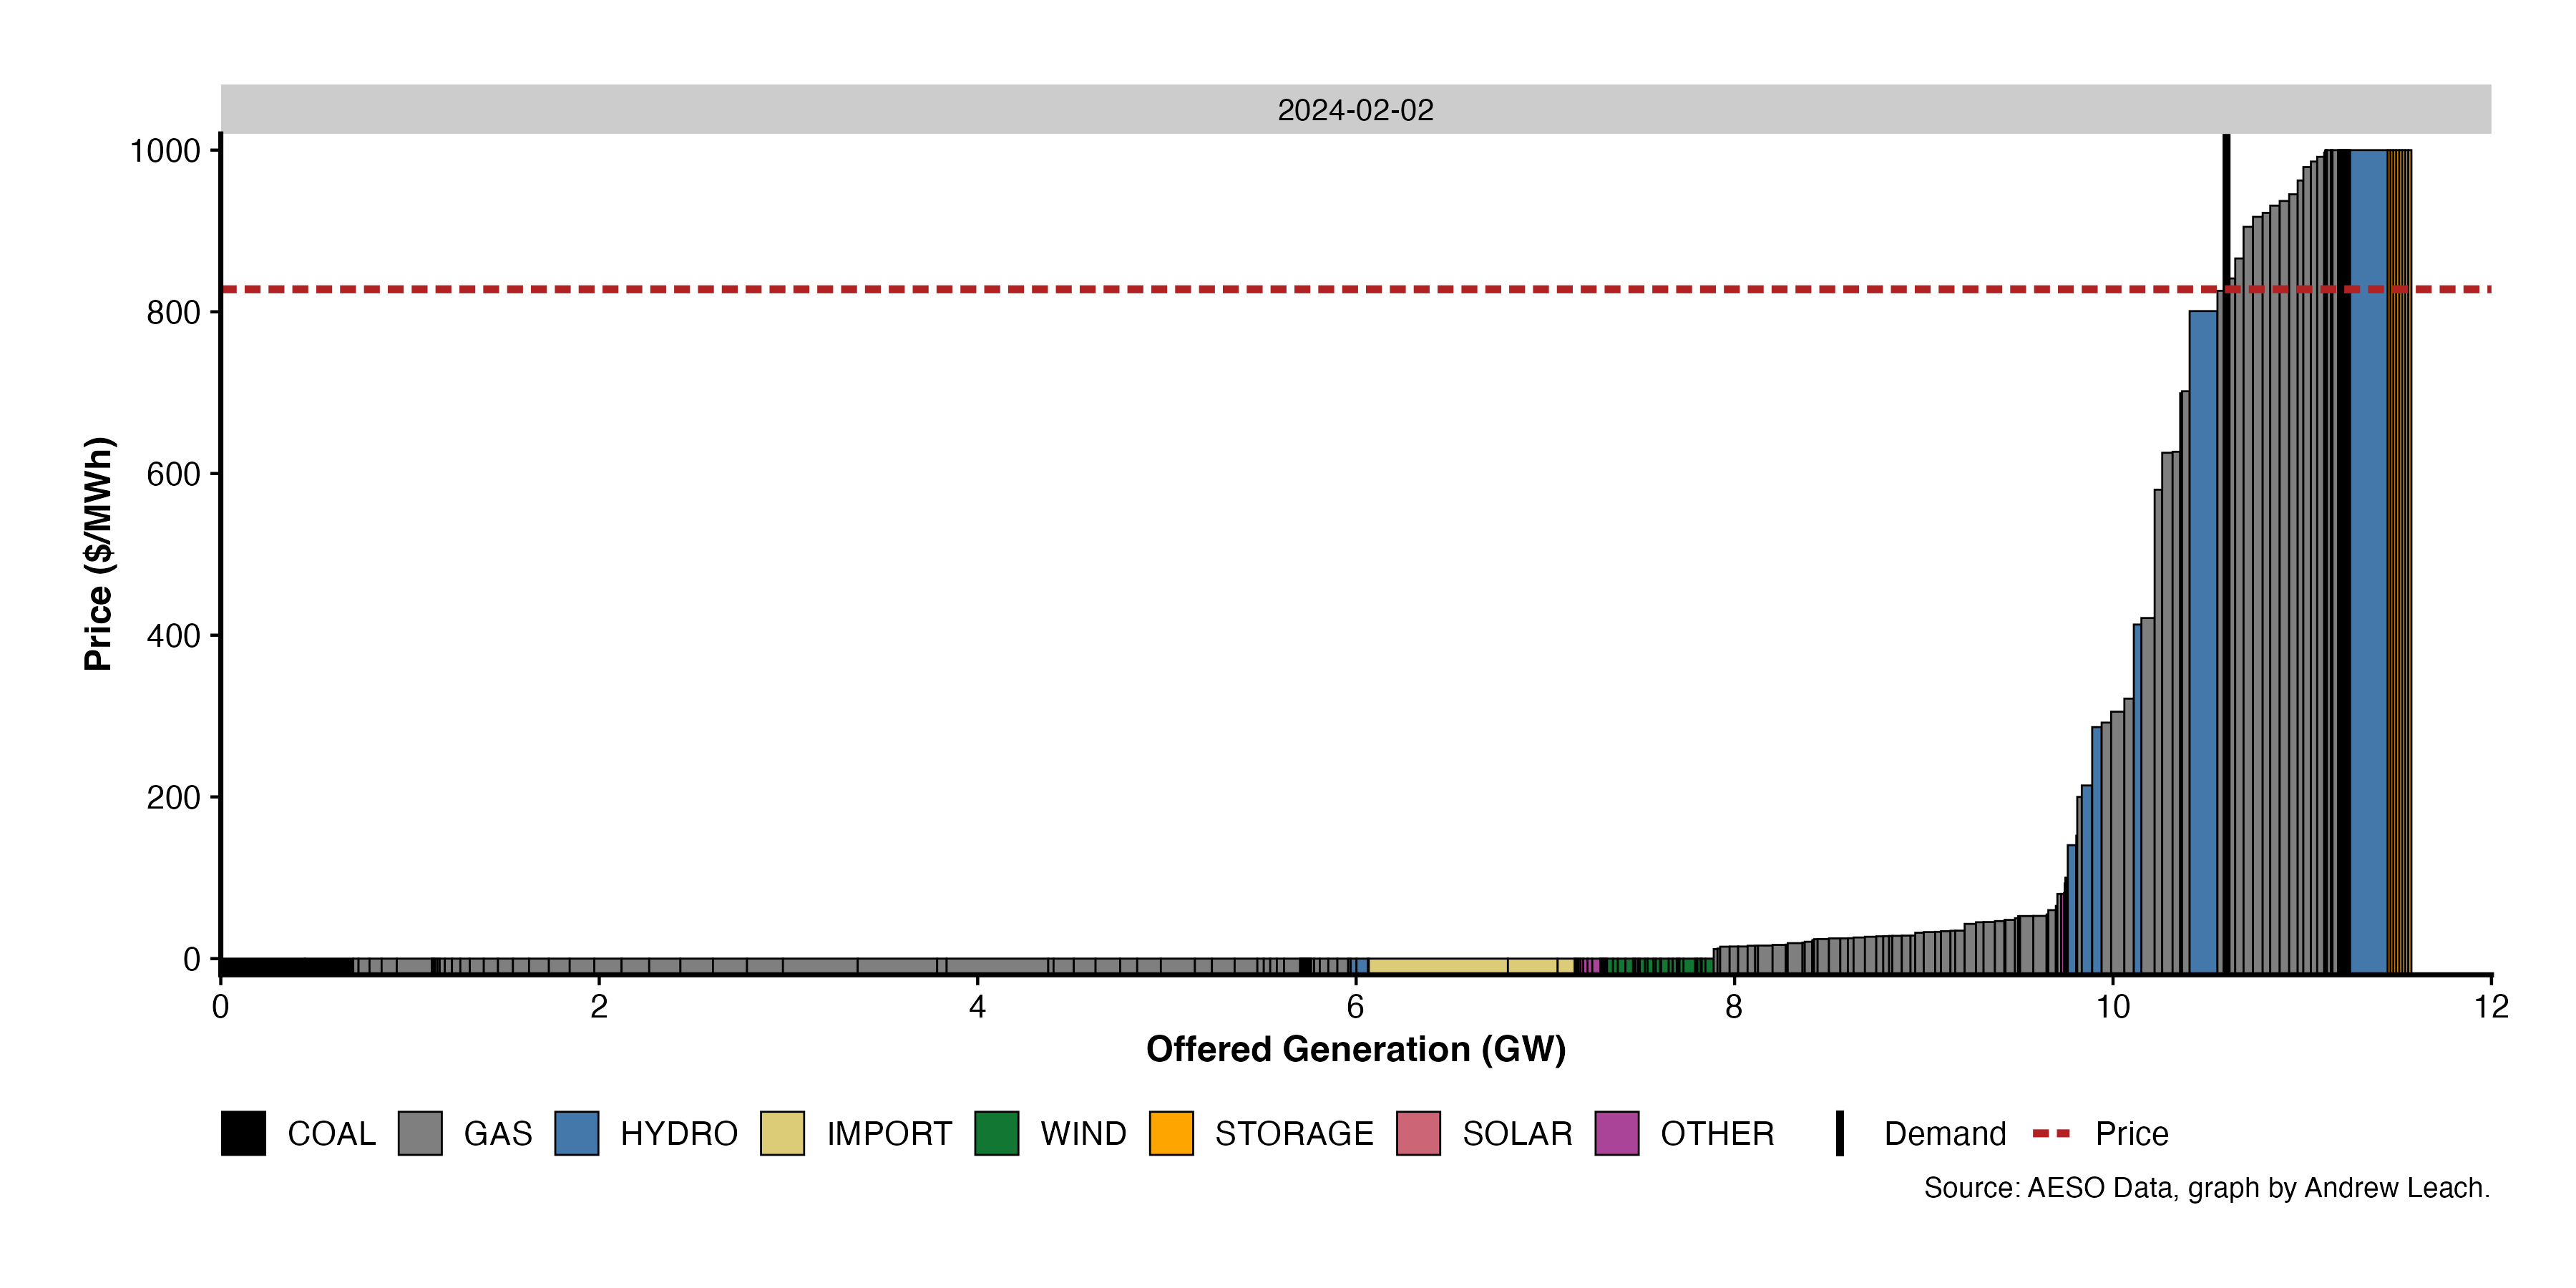
\includegraphics[width=.92\paperwidth]{../images/merit_one_day.png}}; \vspace{1cm}
   \vfill
\end{frame}


\section{Estimation}


\begin{frame}{Estimation Strategy}
    \begin{itemize}
    \item Fundamentally, what we want to do is look at individual merit order blocks and ask to what degree those blocks would have been offered at a different price under different GHG policy parameters
  \end{itemize}
\vfill
\end{frame}



\begin{frame}{Estimation Strategy}
    \begin{itemize}
    \item Fundamentally, what we want to do is look at individual merit order blocks and ask to what degree those blocks would have been offered at a different price under different GHG policy parameters
\item The challenge is that the number of blocks, the size of each block, and the price at which each block is offered is a choice variable for the plant operator
\item And, insofar as carbon pricing affects block size or price, position in the merit order becomes endogenous to carbon pricing
  \end{itemize}
\vfill
\end{frame}


\begin{frame}
   \tikz [remember picture,overlay]
    \node[yshift=-0.3cm,xshift=0cm] at (current page.center)
        {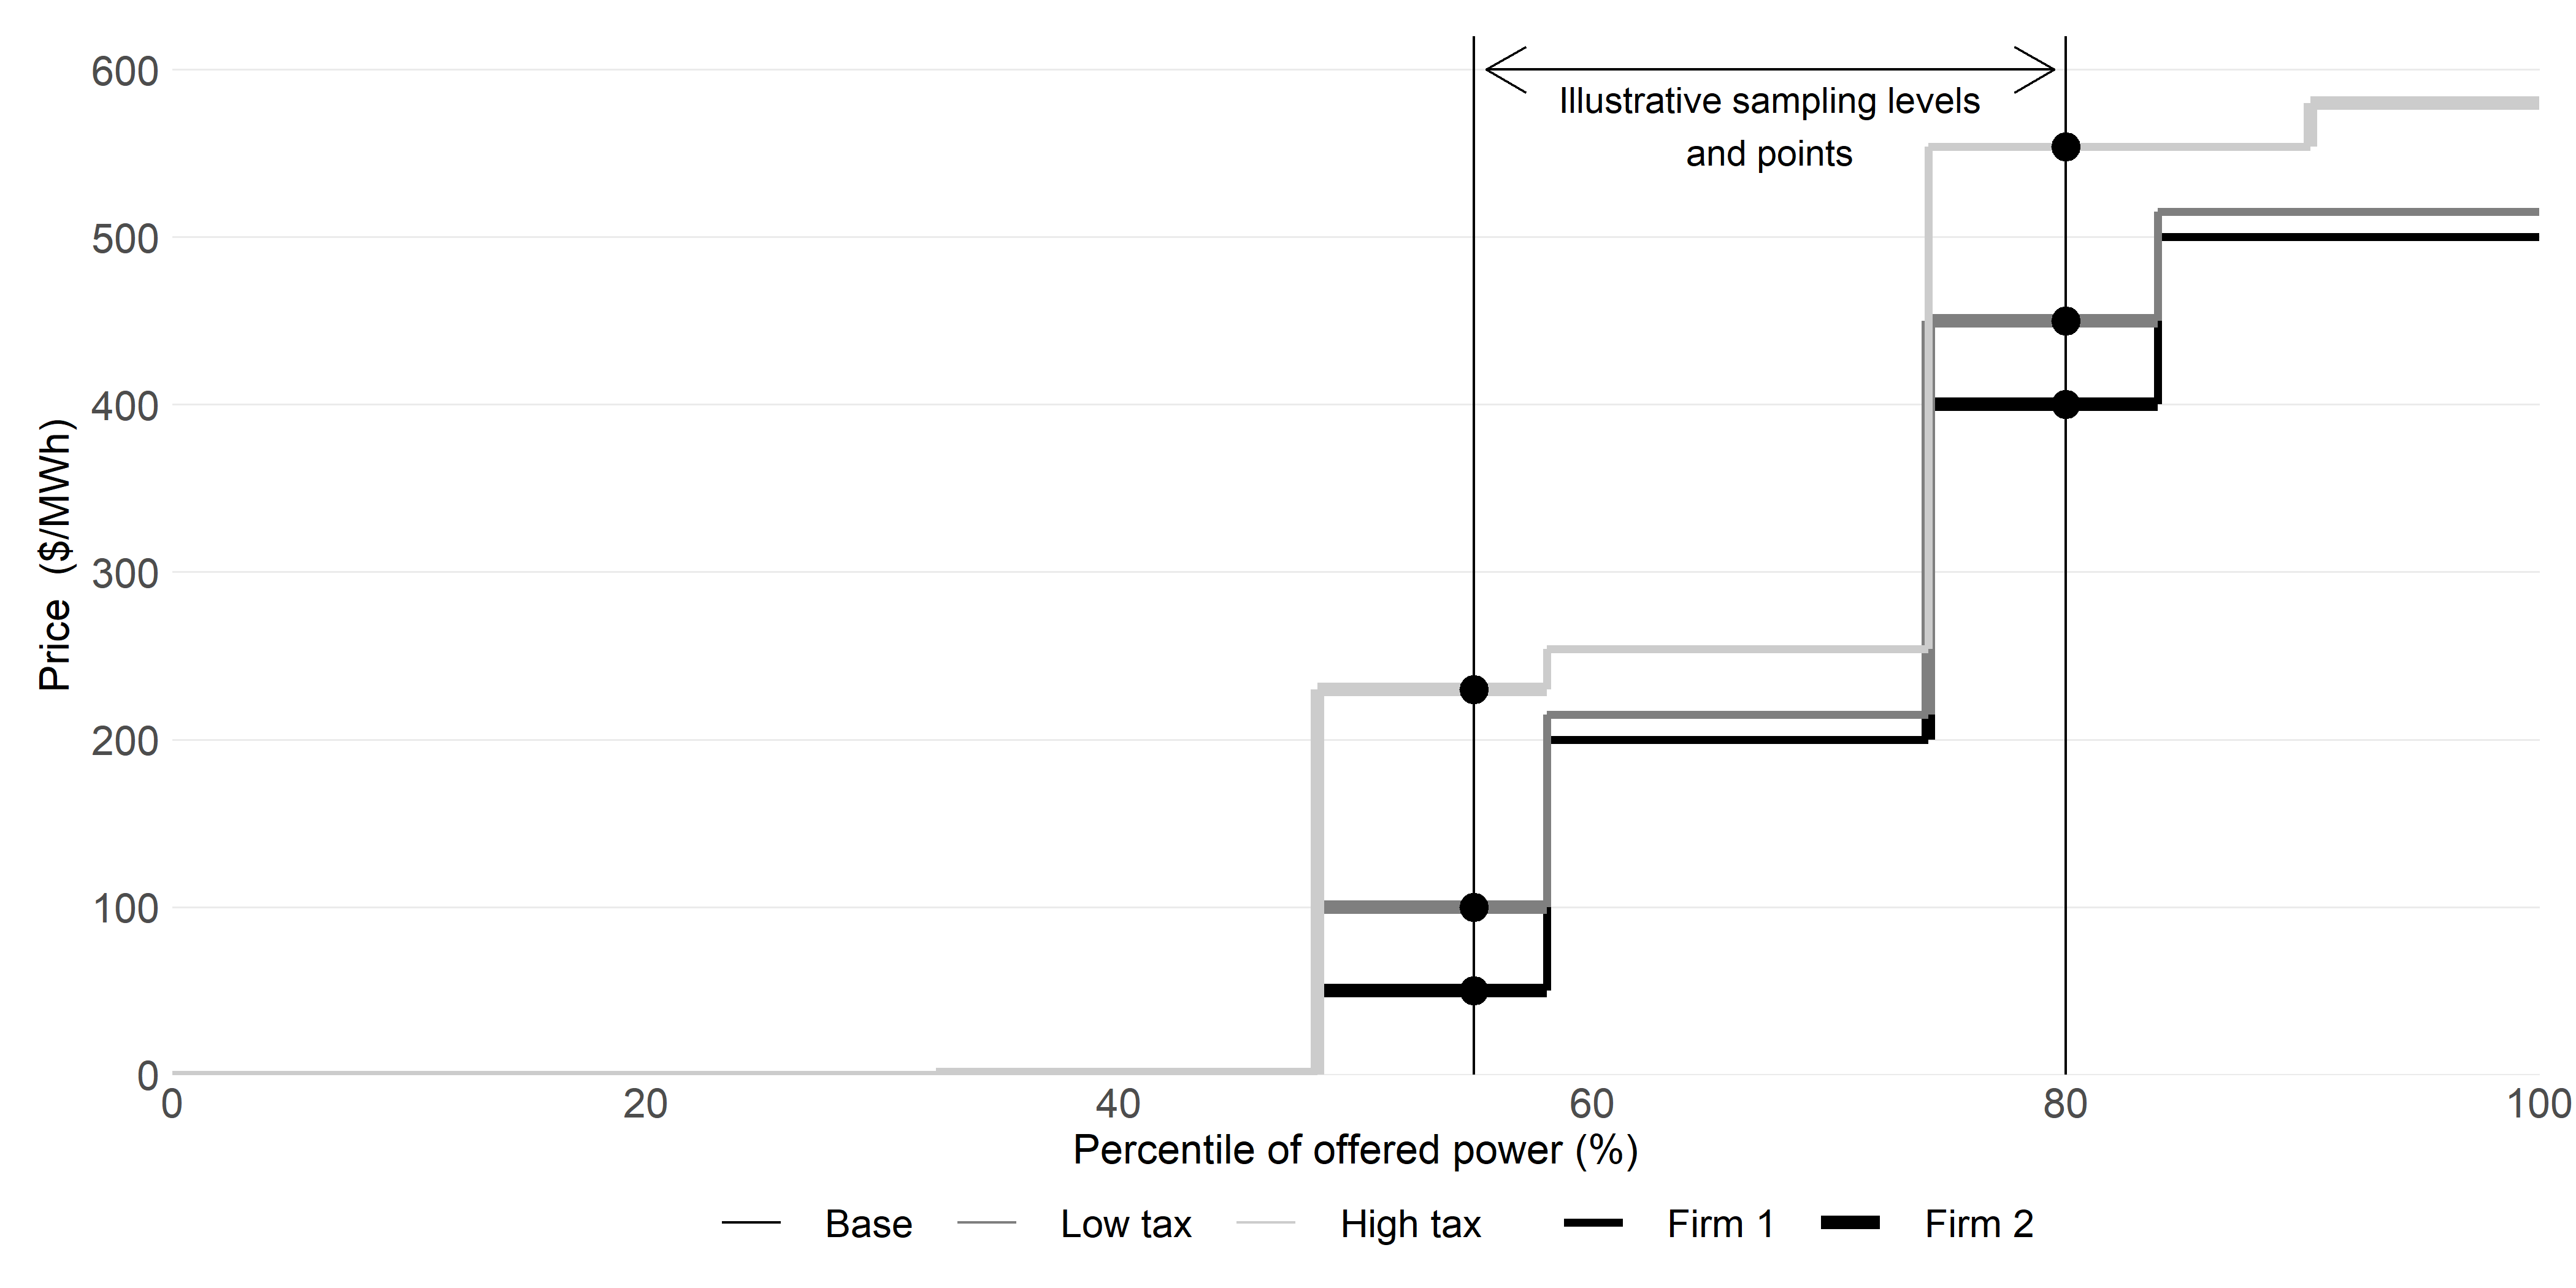
\includegraphics[width=.92\paperwidth]{../images/sampling.png}}; \vspace{1cm}
   \vfill
\end{frame}




\begin{frame}{Estimation Strategy}
    \begin{itemize}
    \item Fundamentally, what we want to do is look at individual merit order blocks and ask to what degree those blocks would have been offered at a different price under different GHG policy parameters
\item The challenge is that the number of blocks, the size of each block, and the price at which each block is offered is a choice variable for the plant operator
\item And, insofar as carbon pricing affects block size or price, position in the merit order becomes endogenous to carbon pricing
\item I use an approach whereby I sample points along the supply curve at a set of percentiles of offered power in every hour in my data set
\item Each sample consists of information about that point in time in the market (percentile, date, time, plant, price, offer control) 
\item Sampling is locally random because of the variability of wind and solar  - a firm could not choose to be consistently at a given percentile in the merit order
  \end{itemize}
\vfill
\end{frame}

\begin{frame}{Merit Order Sampling}
  \tikz[remember picture,overlay] {
    \node[yshift=-0.3cm, xshift=-0.25\paperwidth] at (current page.center)
      {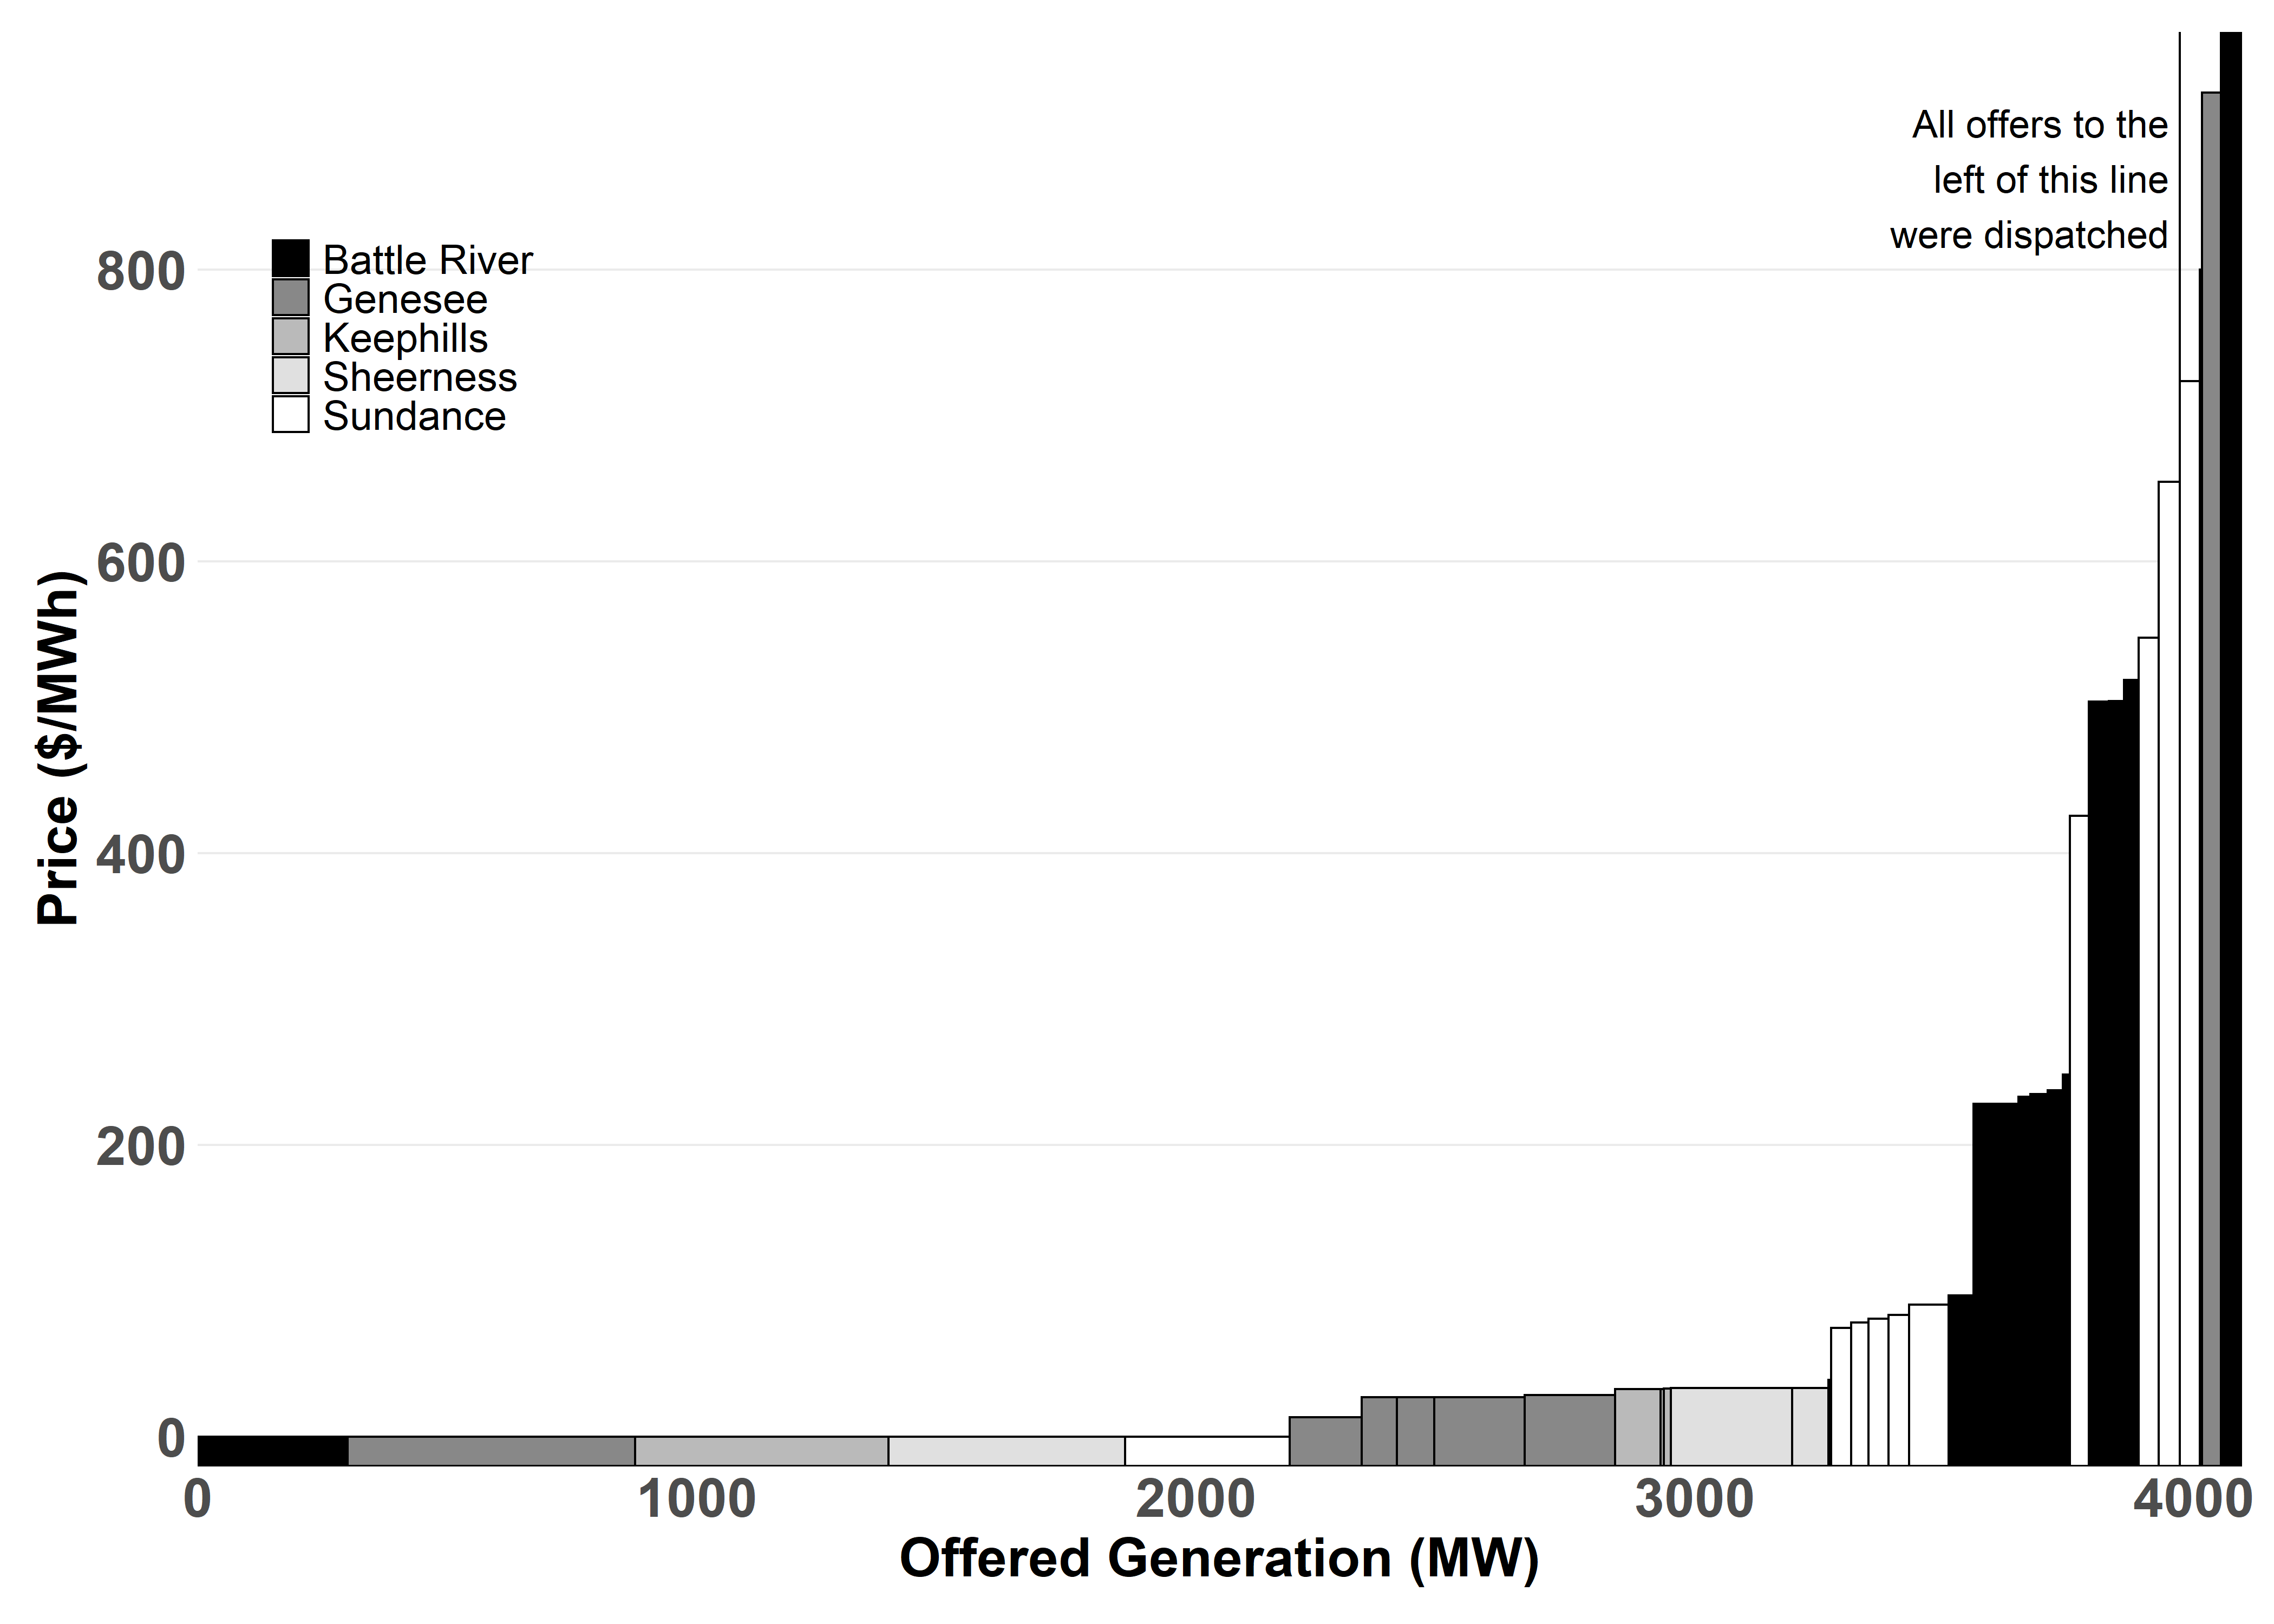
\includegraphics[width=0.46\paperwidth]{../images/coal_merit.png}};
    \node[yshift=-0.3cm, xshift=0.25\paperwidth] at (current page.center)
      {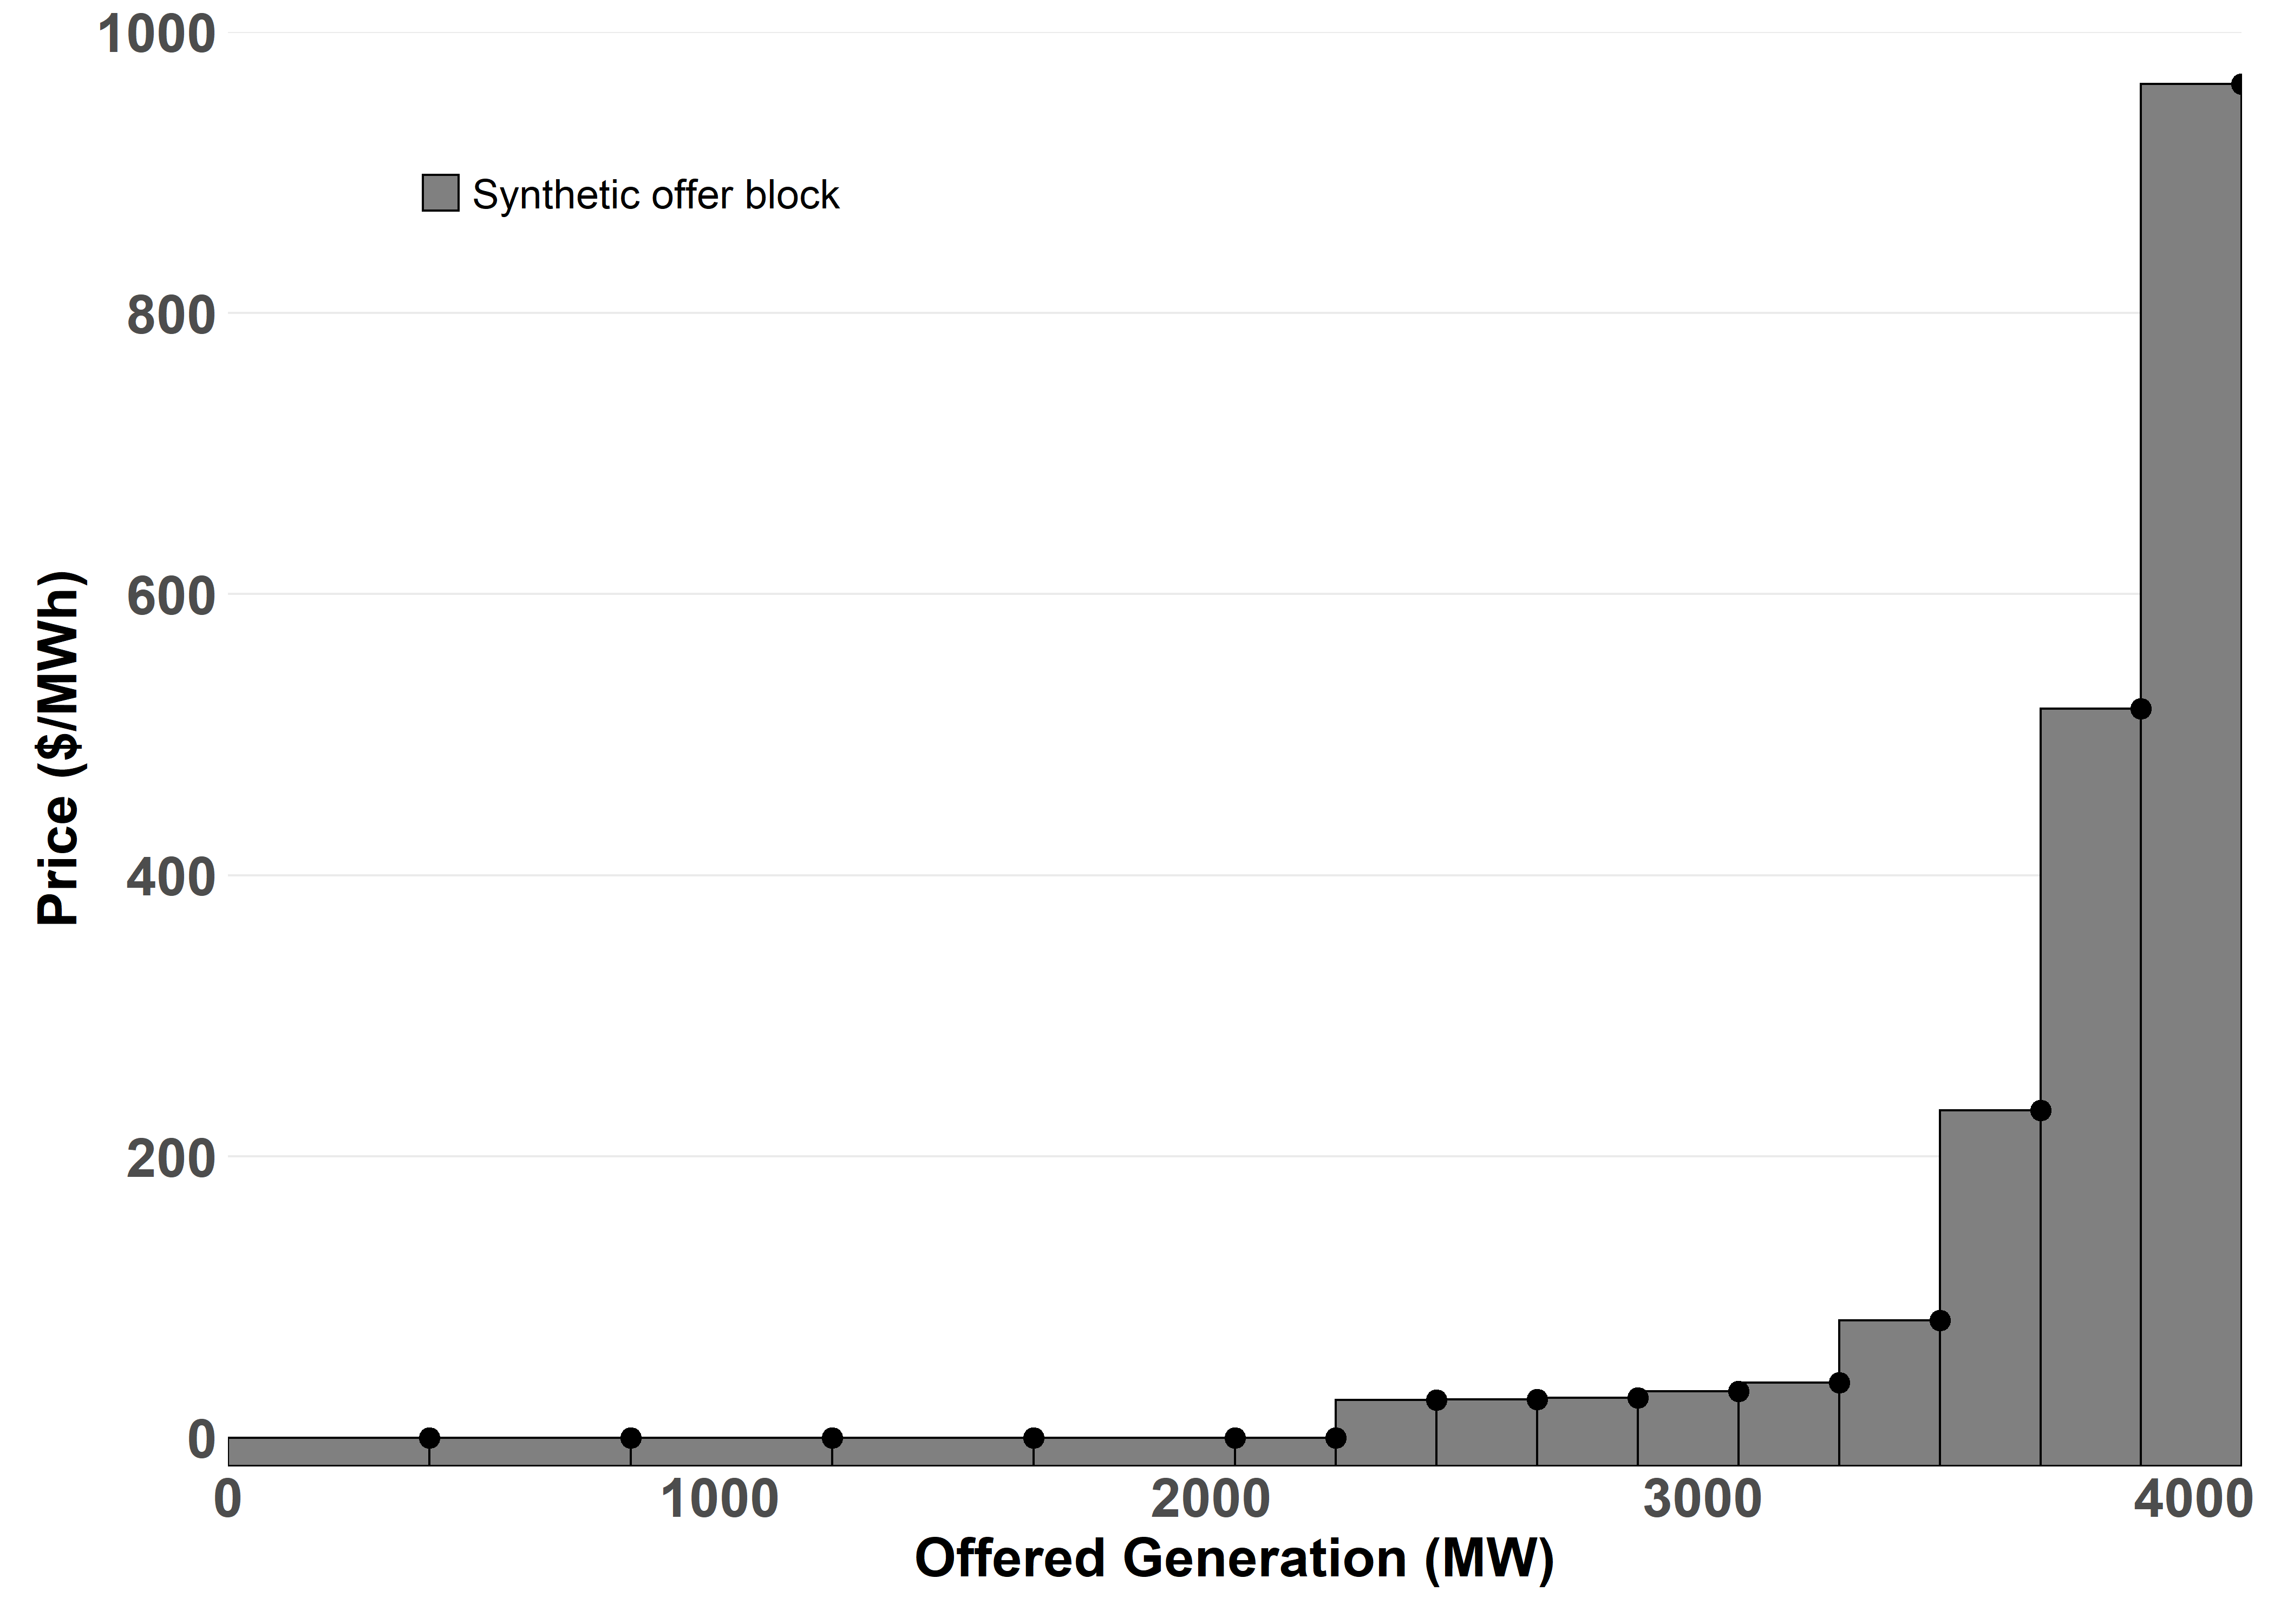
\includegraphics[width=0.46\paperwidth]{../images/coal_synth_merit.png}};
  }
\end{frame}




\begin{frame}{Merit Order Sampling with Coal Offers}
  \tikz[remember picture,overlay] {
    \node[yshift=-0.3cm, xshift=-0.25\paperwidth] at (current page.center)
      {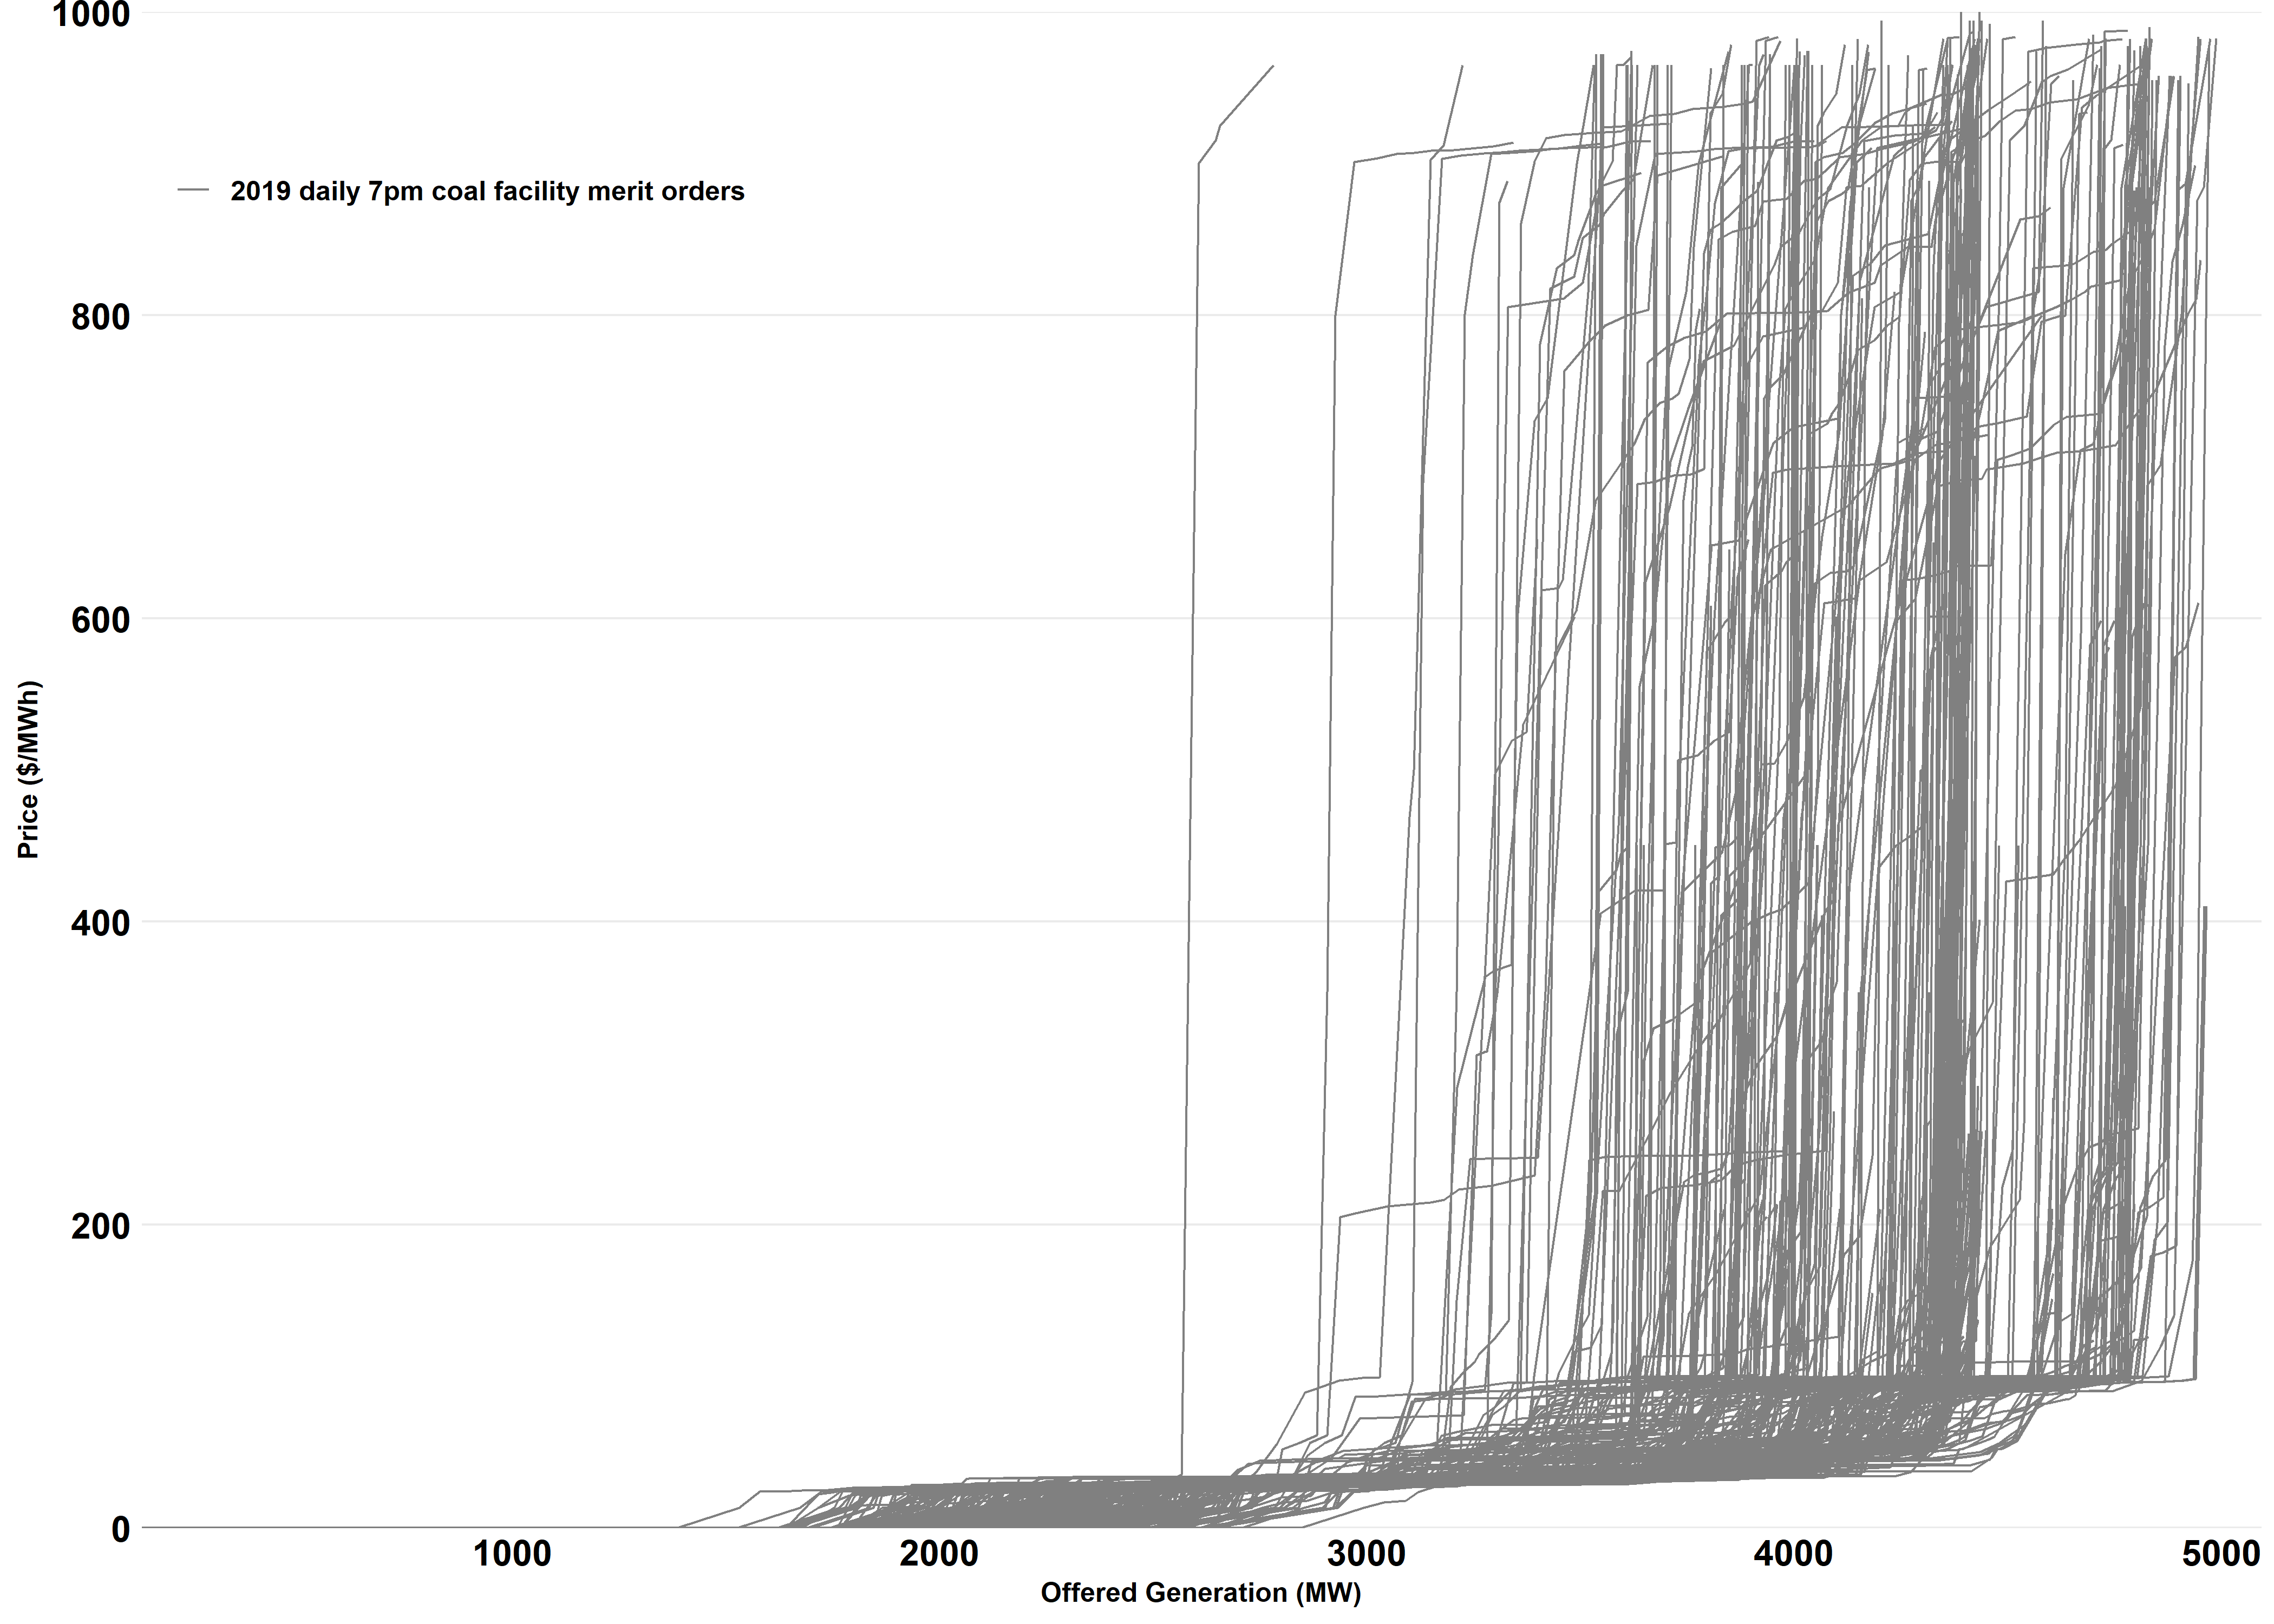
\includegraphics[width=0.42\paperwidth]{../images/all_coal_merit.png}};
    \node[yshift=-0.3cm, xshift=0.25\paperwidth] at (current page.center)
      {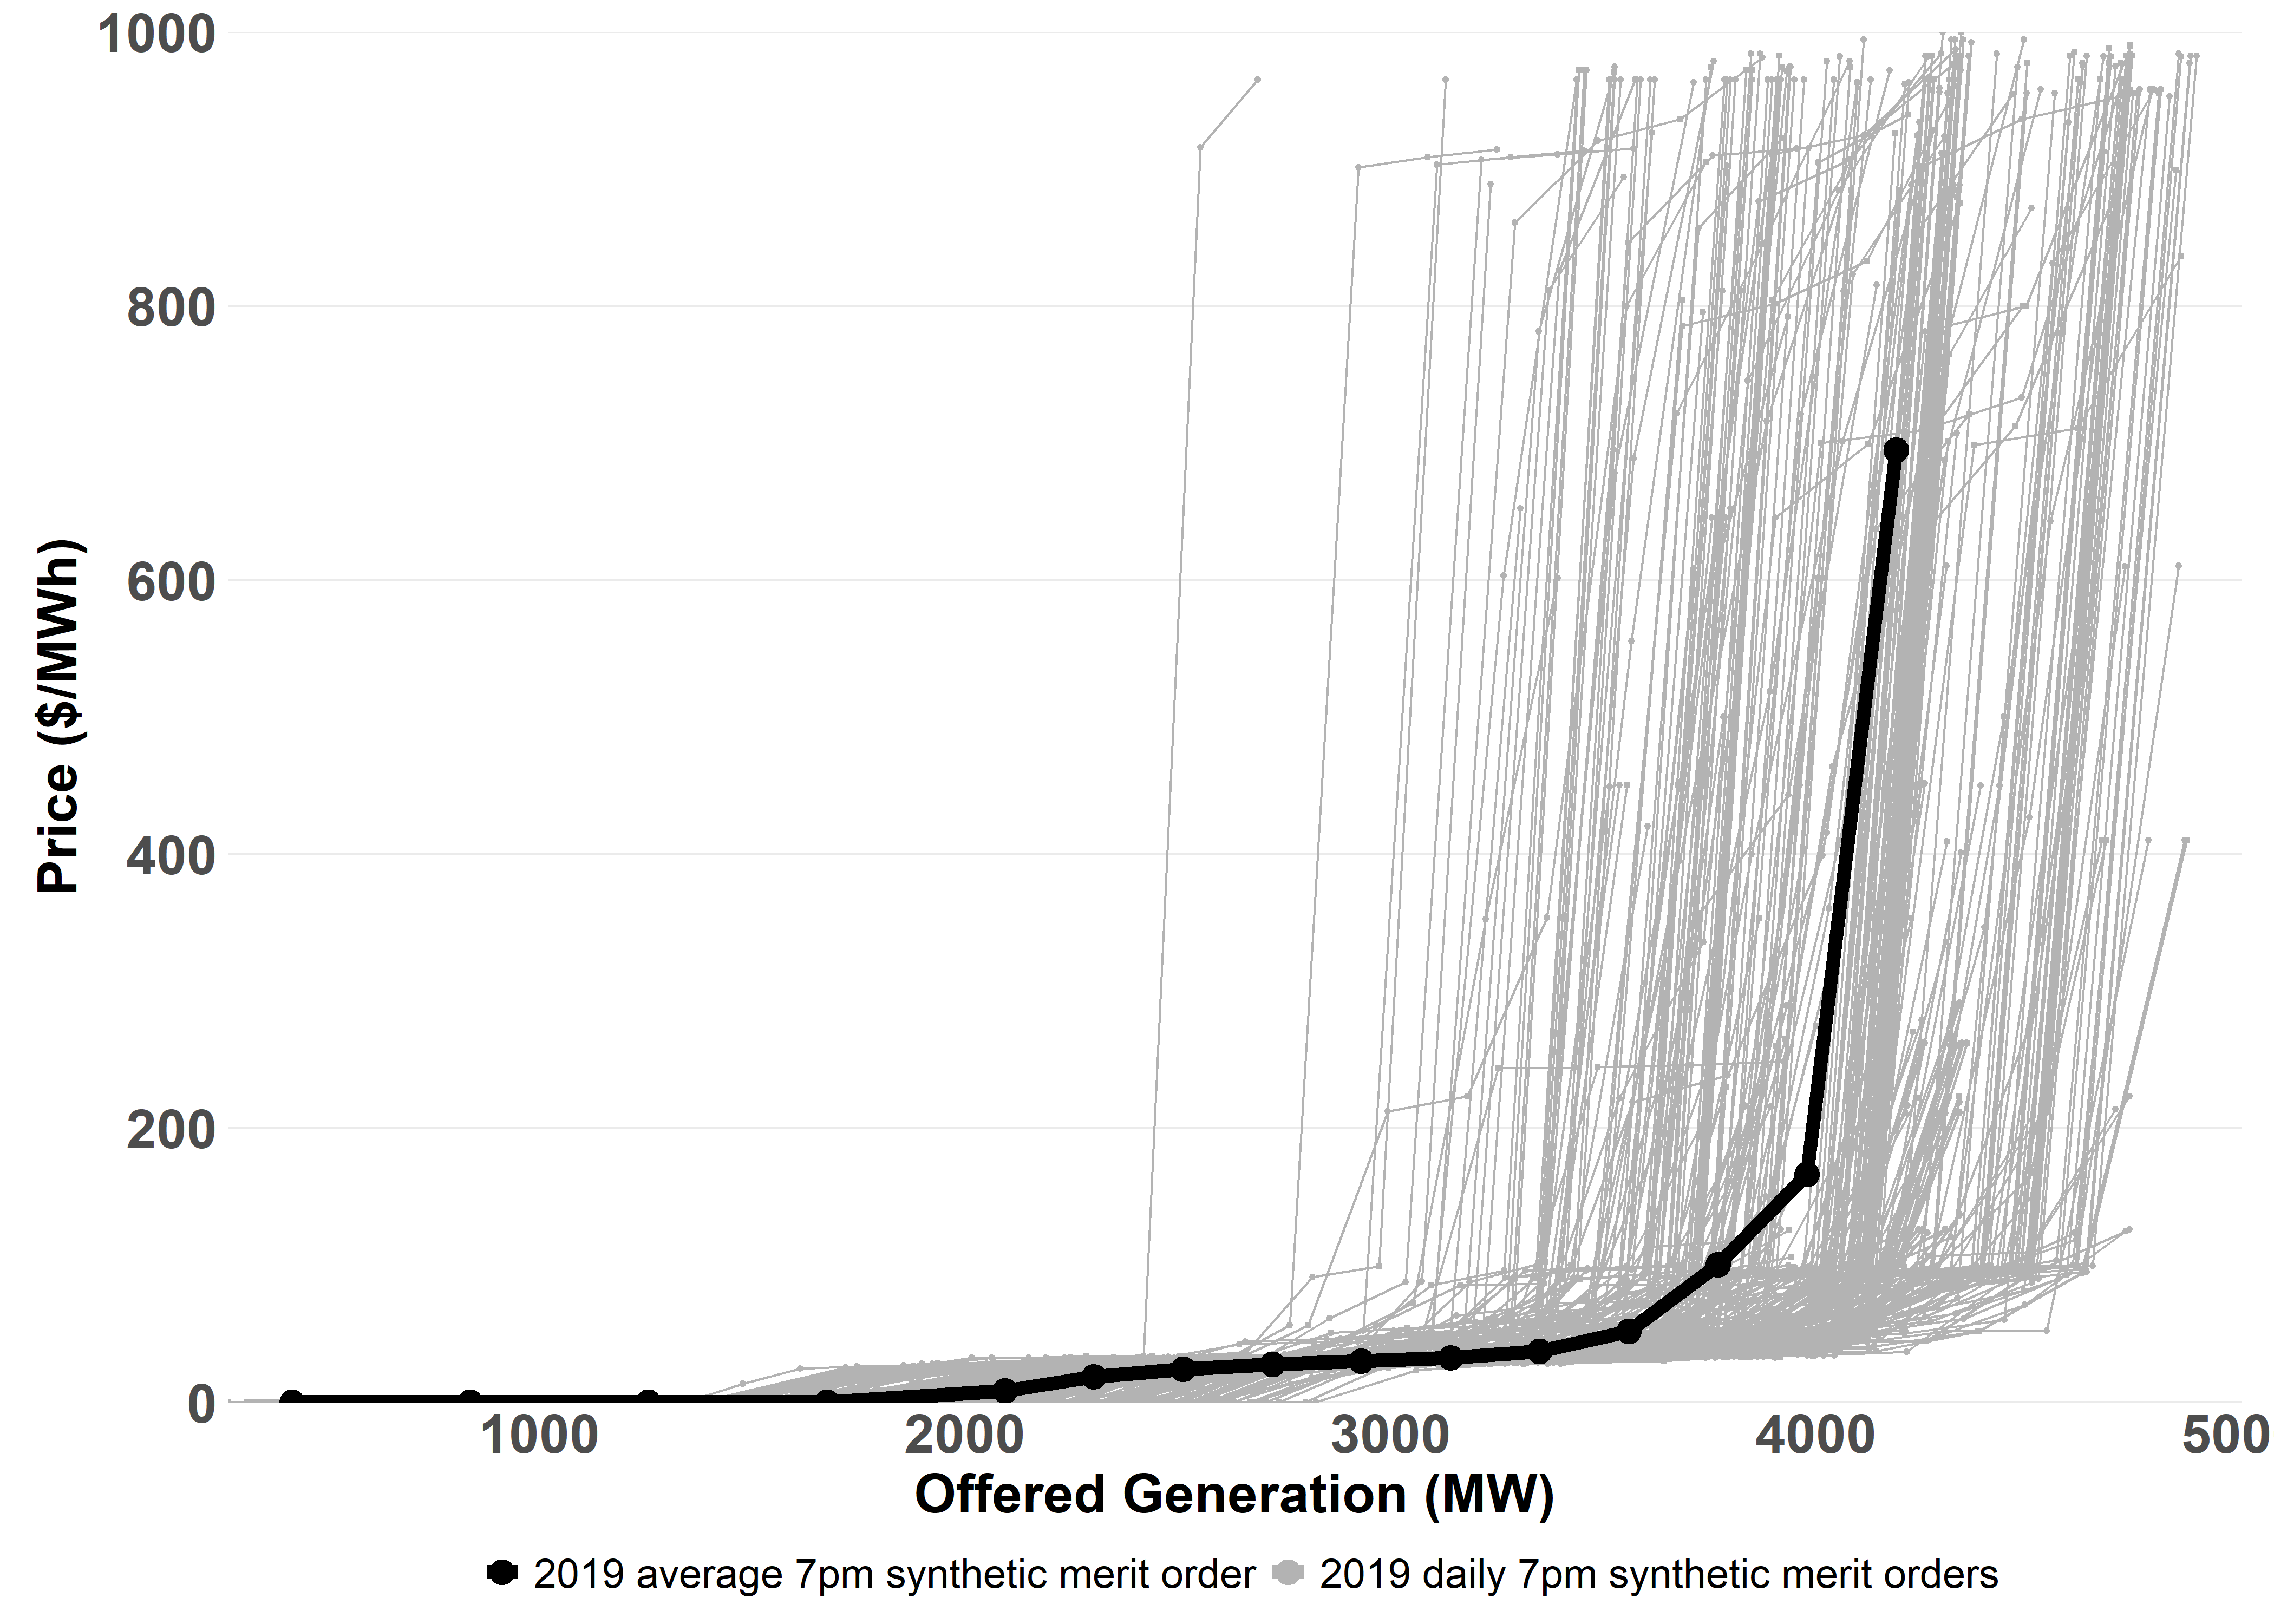
\includegraphics[width=0.42\paperwidth]{../images/coal_synth_2019.png}};
  }
\end{frame}


\begin{frame}{Nested Percentile Regressions}
\begin{itemize}
\item Variation in carbon pricing over time and variation in emissions-intensity across facilities allows identification of the effect of carbon pricing on the sampled points in the merit order
 \item Each sampled point contains facility ($F$) and market ($M$) information, as well as carbon policy compliance costs
\end{itemize}
The estimation equation is then: 
\begin{align*}
 \underbrace{P_{j,t}}_{\substack{\text{Offer value} \\ \text{at percentile }j\\ \text{at time }t}}&=
 \underbrace{\alpha_{j}}_{\substack{\text{Constant for} \\ \text{percentile }j}}+
 \underbrace{\beta_j M_t}_{\substack{\text{Market, policy, and} \\ \text{climate variables} \\\text{at time }t}}+
 \underbrace{\delta_j F_{j,t}}_{\substack{\text{Facility} \\ \text{characteristics} \\ \text{at percentile }j\\ \text{at time }t}}+
 \underbrace{\zeta_j t_{j,t}}_{\substack{\text{Carbon cost} \\ \text{at percentile j}\\ \text{at time }t}}+
 \underbrace{\kappa_j O_{j,t}}_{\substack{\text{OBA value} \\ \text{at percentile j}\\ \text{at time }t}}+
 \underbrace{\epsilon_{j,t}.}_{\substack{\text{Error term}}}
\end{align*}
\vfill
\end{frame}


\begin{frame}
   \tikz [remember picture,overlay]
    \node[yshift=-0.3cm,xshift=0cm] at (current page.center)
        {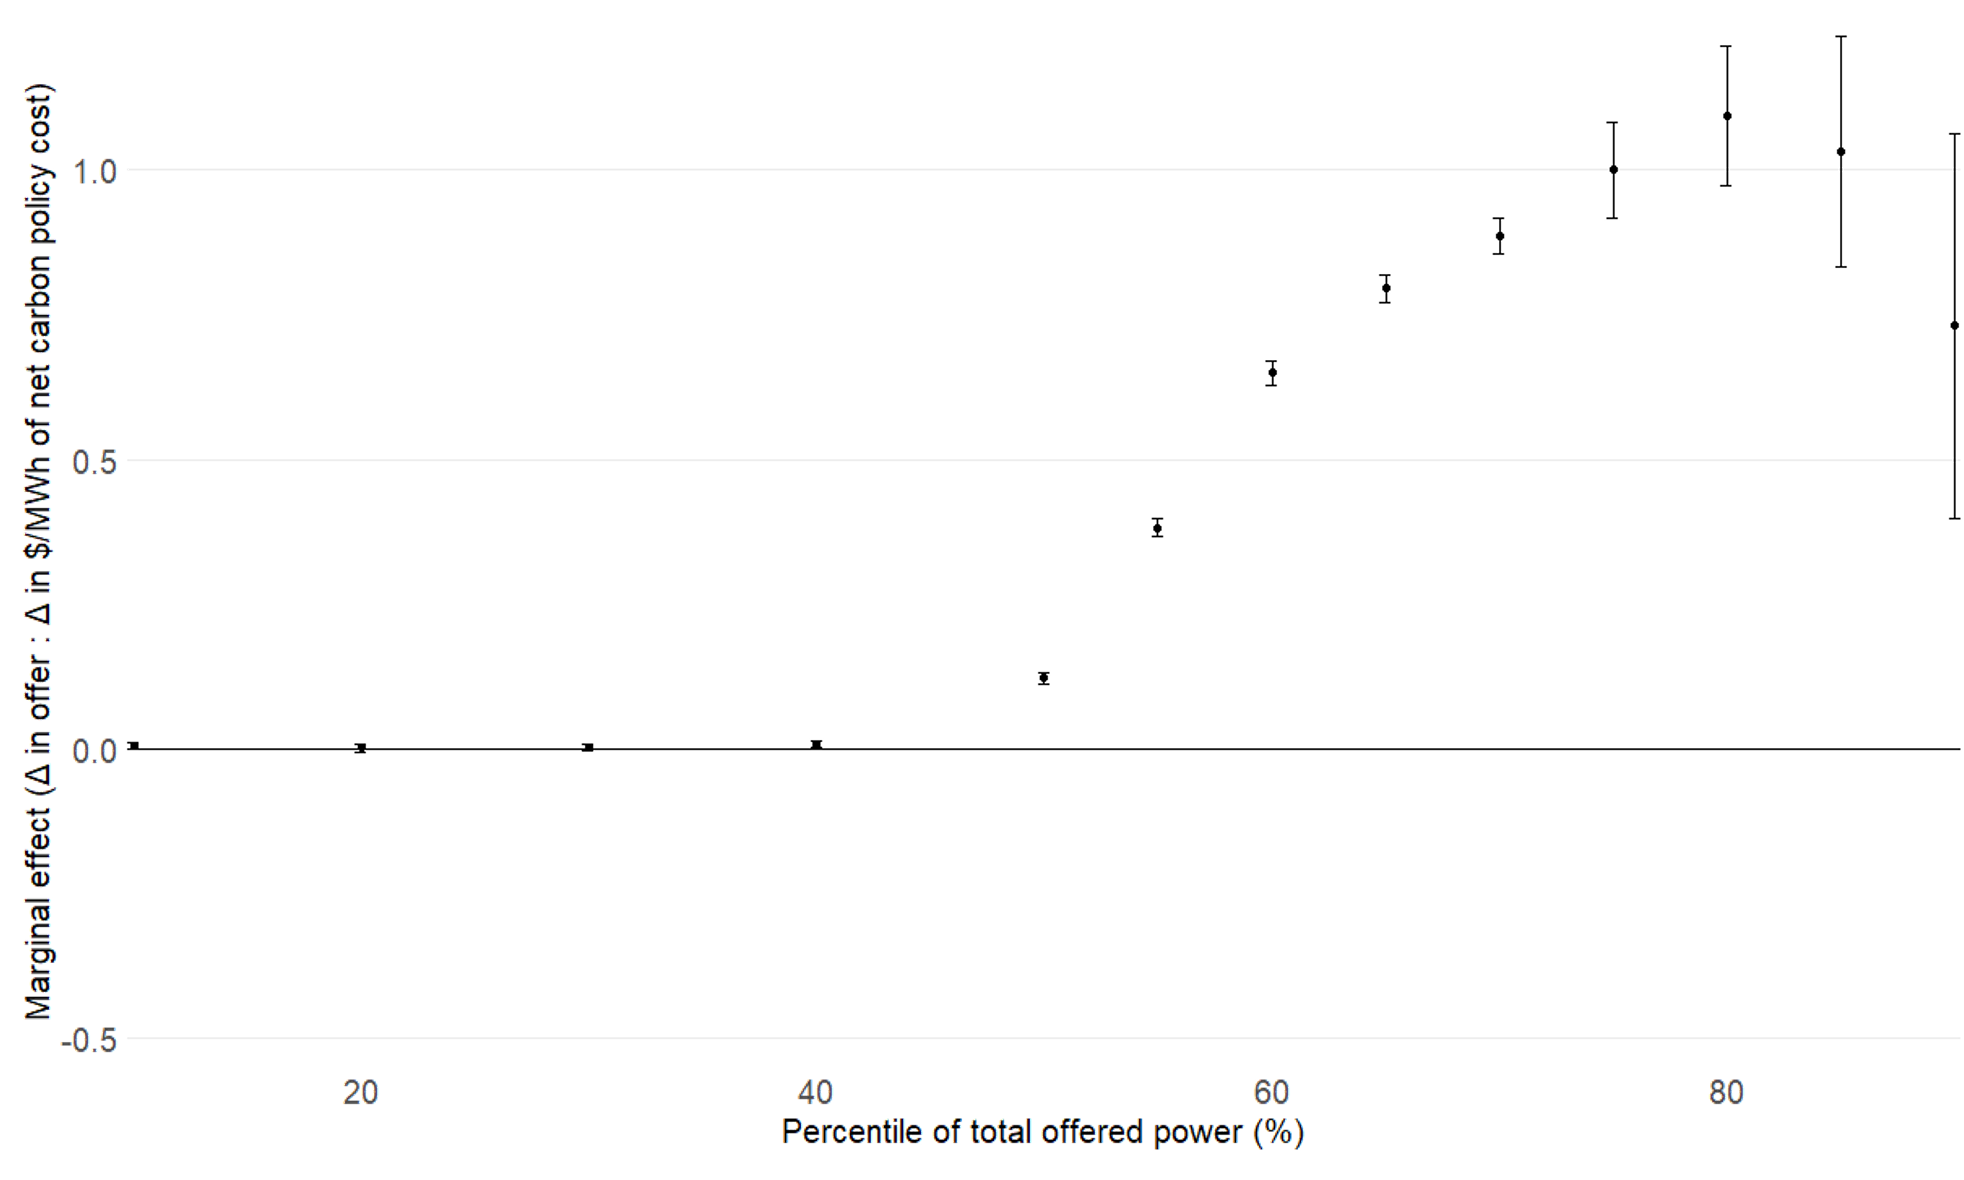
\includegraphics[width=.80\paperwidth]{../images/expectation.png}}; \vspace{1cm}
   \vfill
\end{frame}


\begin{frame}{Close...in a few cases}
   \tikz [remember picture,overlay]
    \node[yshift=-0.8cm,xshift=0cm] at (current page.center)
        {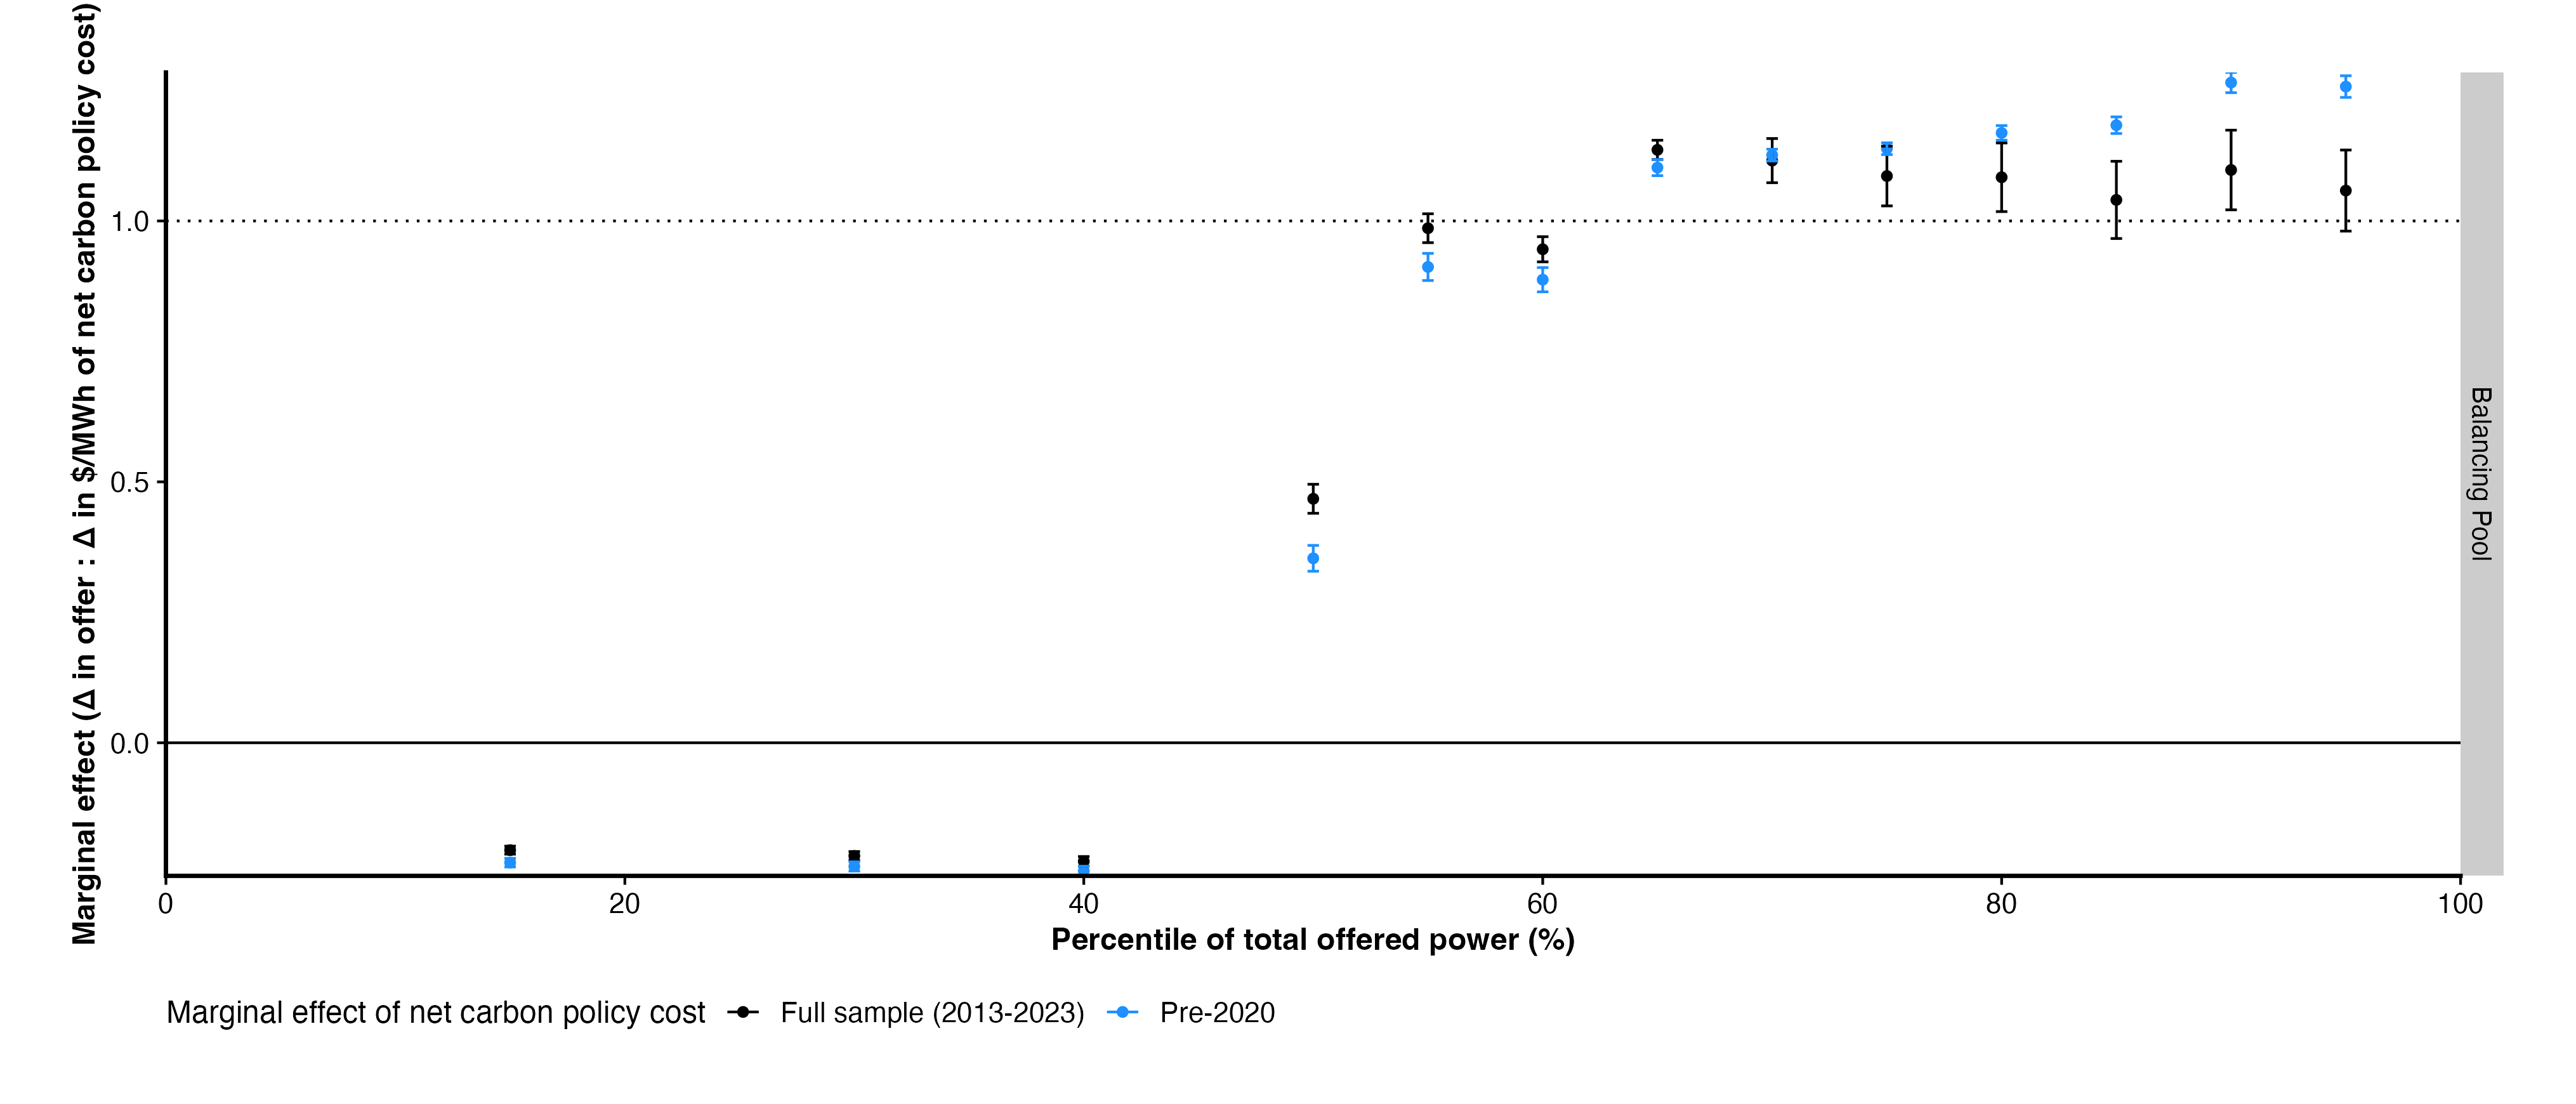
\includegraphics[width=.95\paperwidth]{../images/offers_bp.png}}; \vspace{1cm}
   \vfill
\end{frame}


\section{Results}

\begin{frame}{Net impact of carbon pricing, all firms, all hours}
   \tikz [remember picture,overlay]
    \node[yshift=-0.4cm,xshift=0cm] at (current page.center)
        {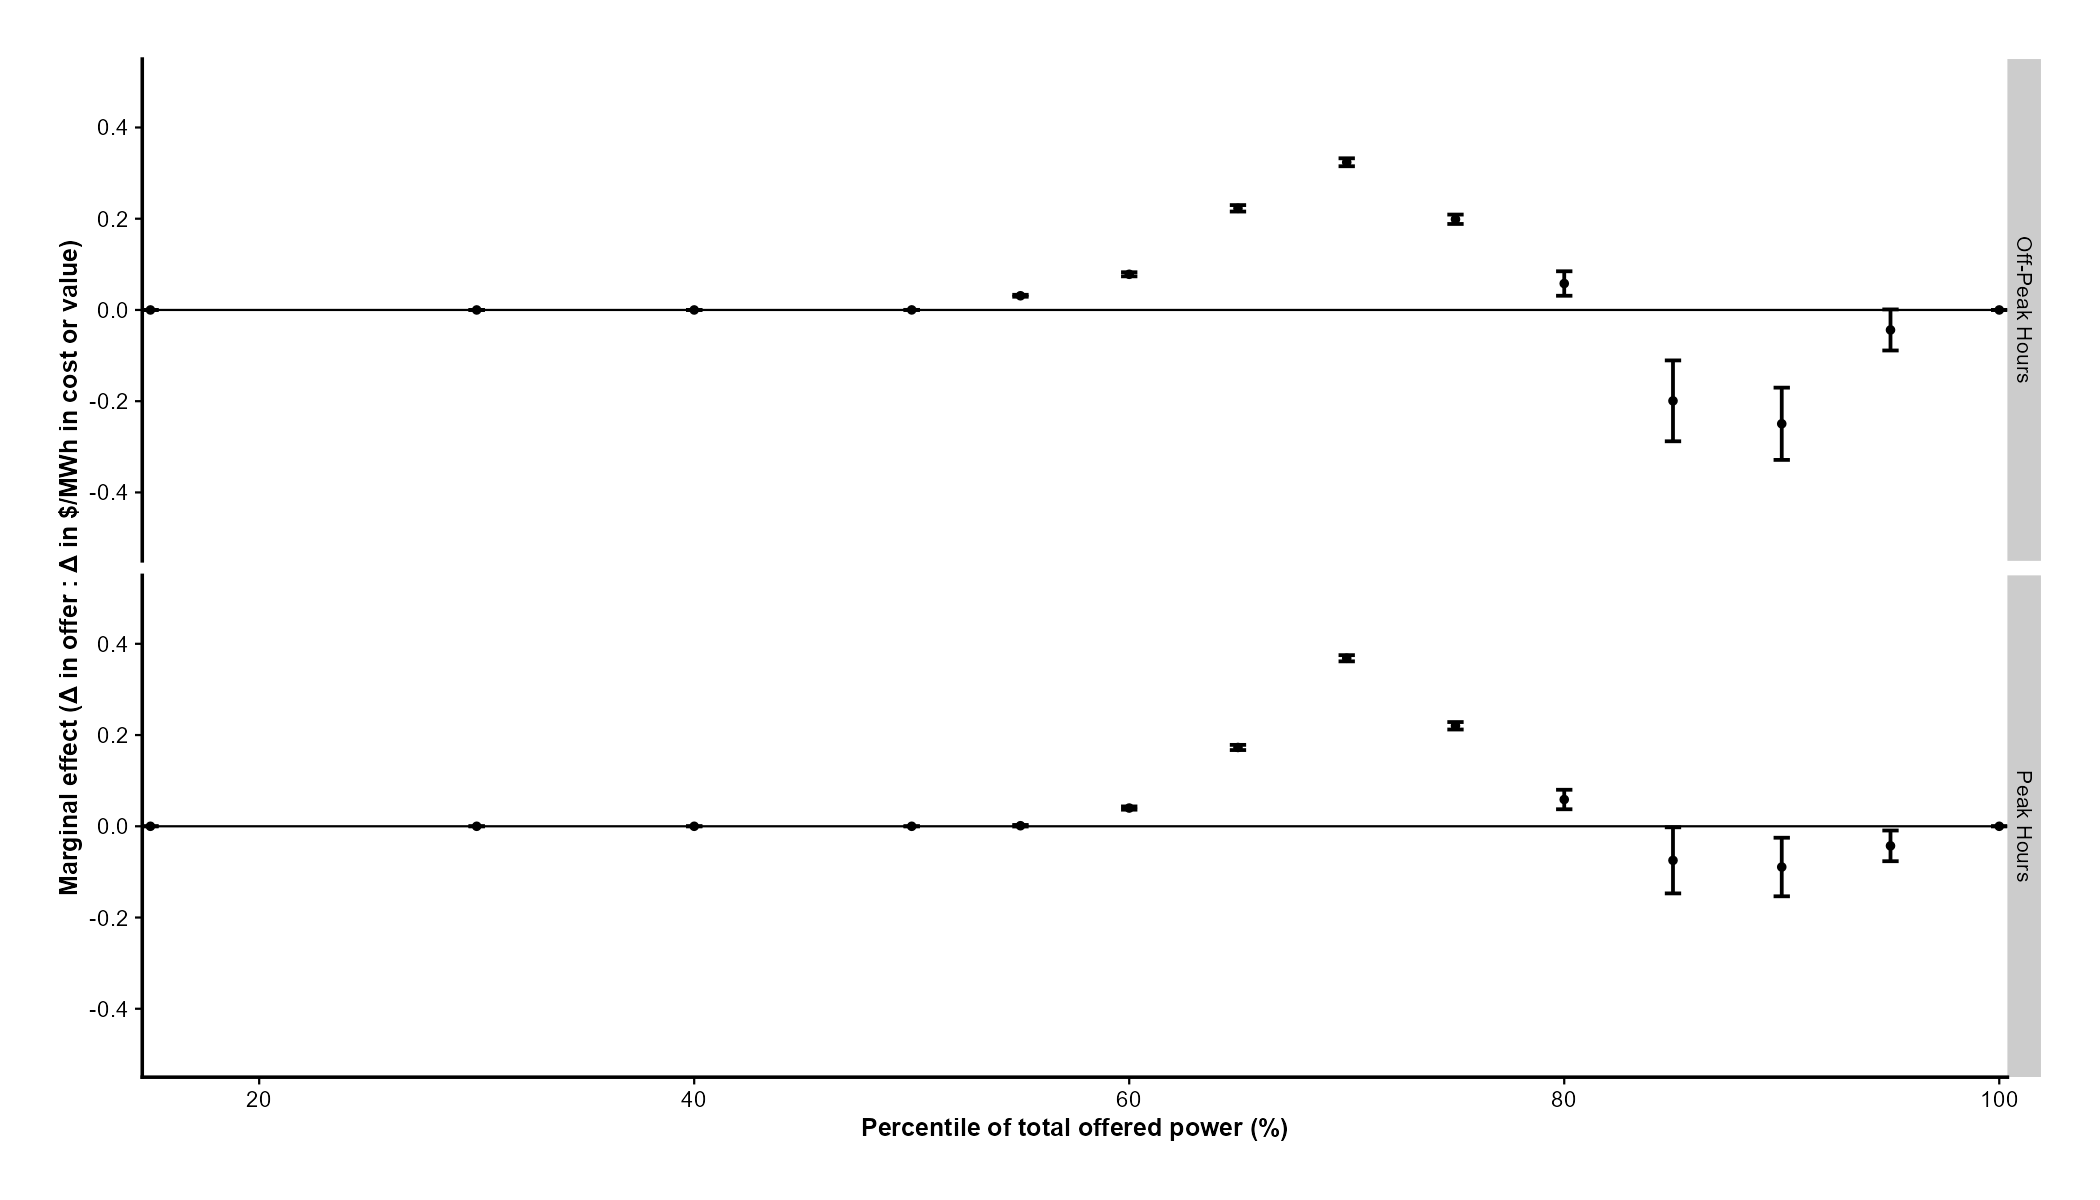
\includegraphics[width=.8\paperwidth]{../images/all_plants_net_peak.png}}; \vspace{1cm}
   \vfill
\end{frame}


\begin{frame}{Net impact of carbon pricing, all firms, peak vs. off-peak hours}
   \tikz [remember picture,overlay]
    \node[yshift=-0.75cm,xshift=0cm] at (current page.center)
        {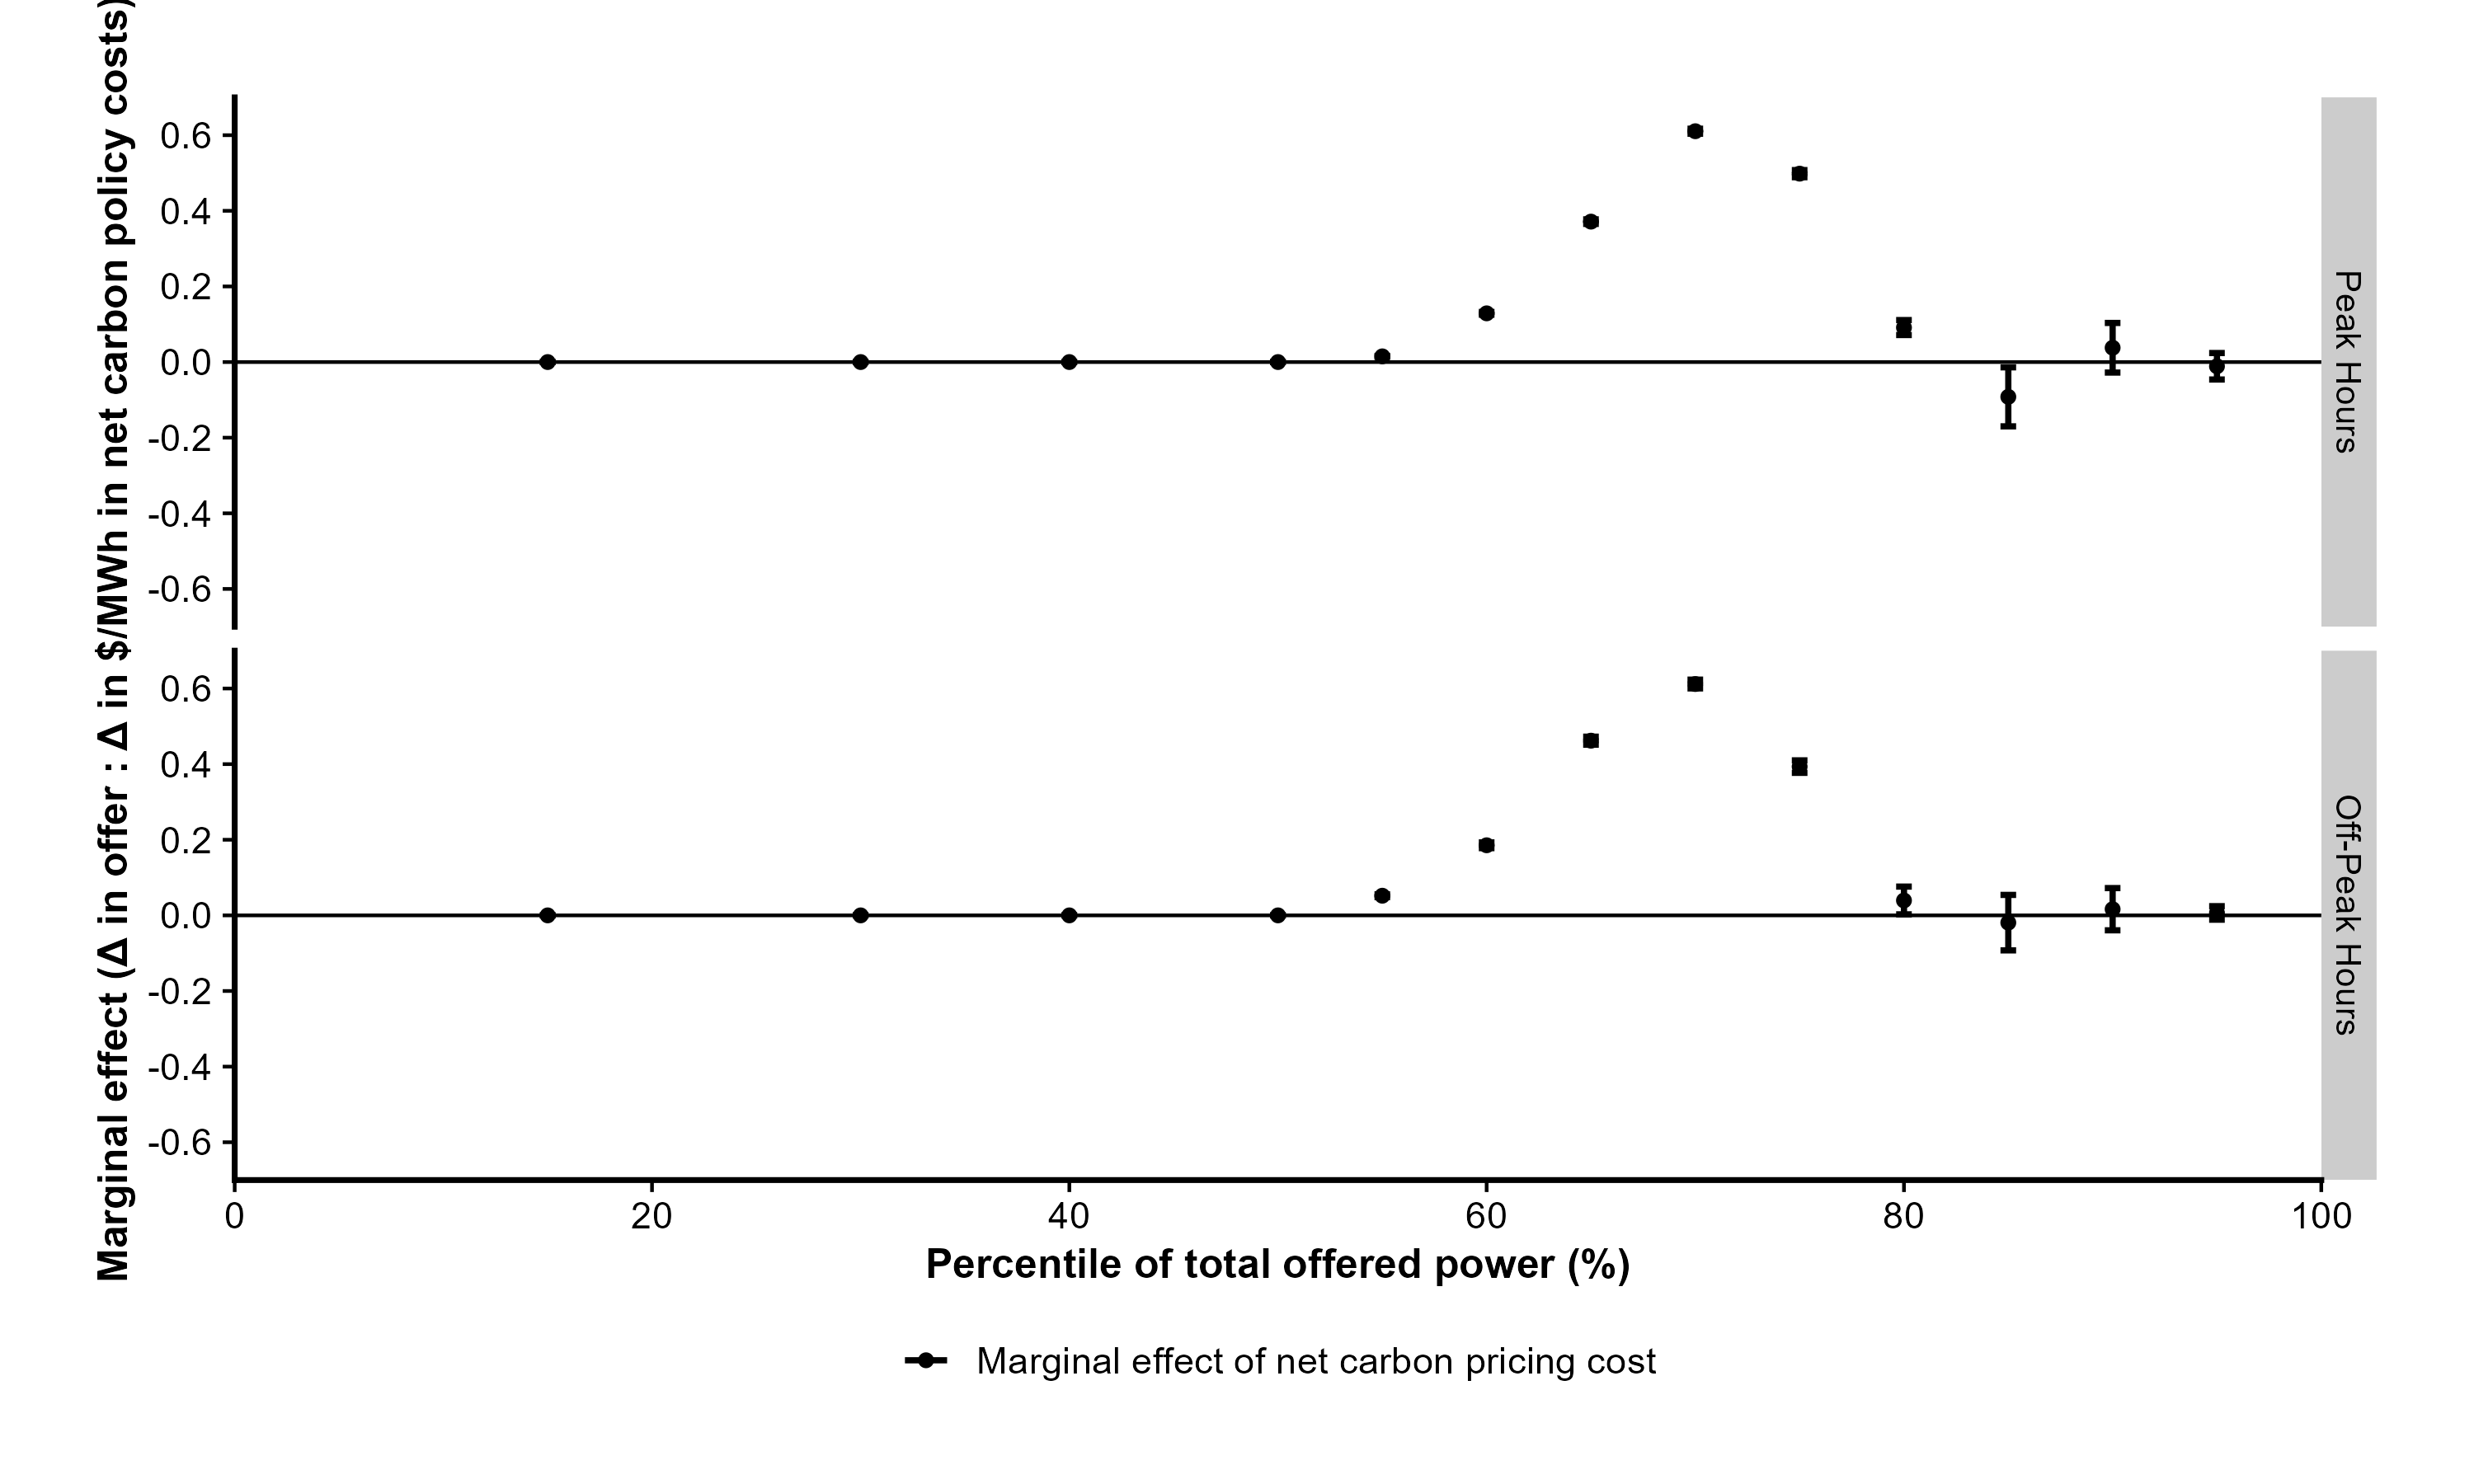
\includegraphics[width=.78\paperwidth]{../images/all_plants_net_peak_flex.png}}; \vspace{1cm}
   \vfill
\end{frame}


\begin{frame}{Decomposition of carbon tax and OBA, all firms, all hours}
   \tikz [remember picture,overlay]
    \node[yshift=-0.6cm,xshift=0cm] at (current page.center)
        {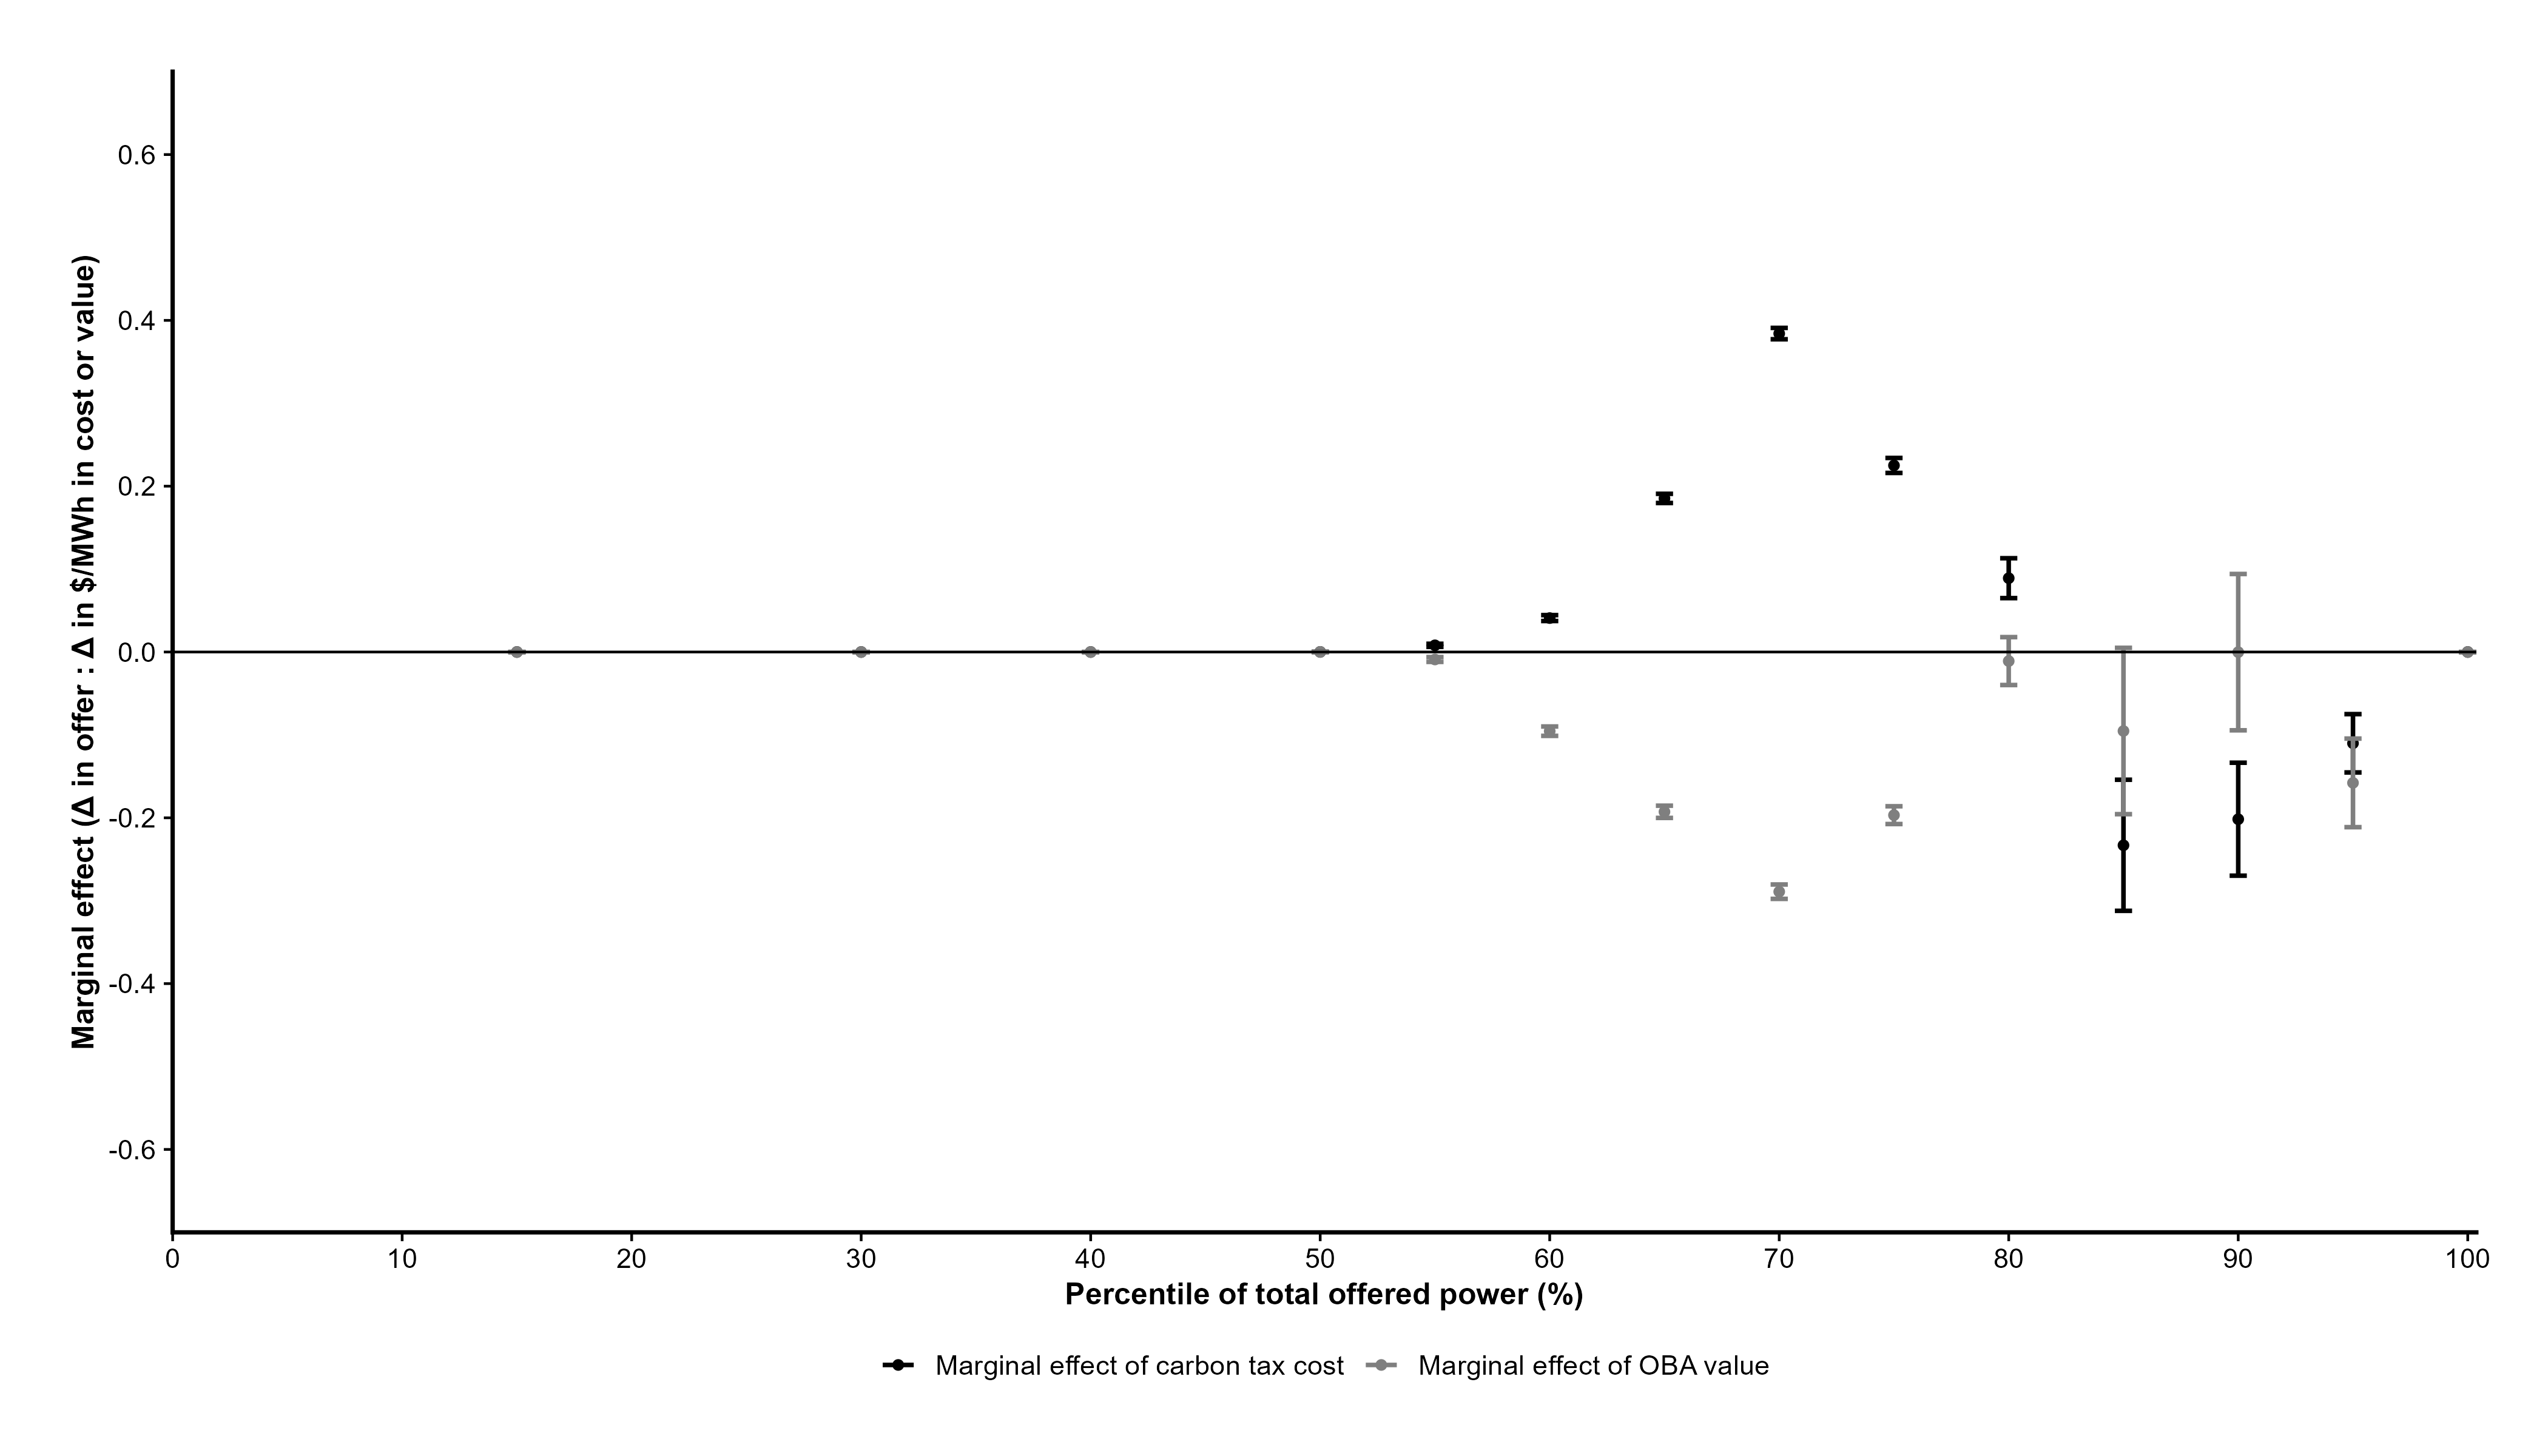
\includegraphics[width=.85\paperwidth]{../images/all_plants_no_peaks.png}}; \vspace{1cm}
   \vfill
\end{frame}

\begin{frame}{Decomposed impacts, all firms, peak vs. off-peak hours}
   \tikz [remember picture,overlay]
    \node[yshift=-0.6cm,xshift=0cm] at (current page.center)
        {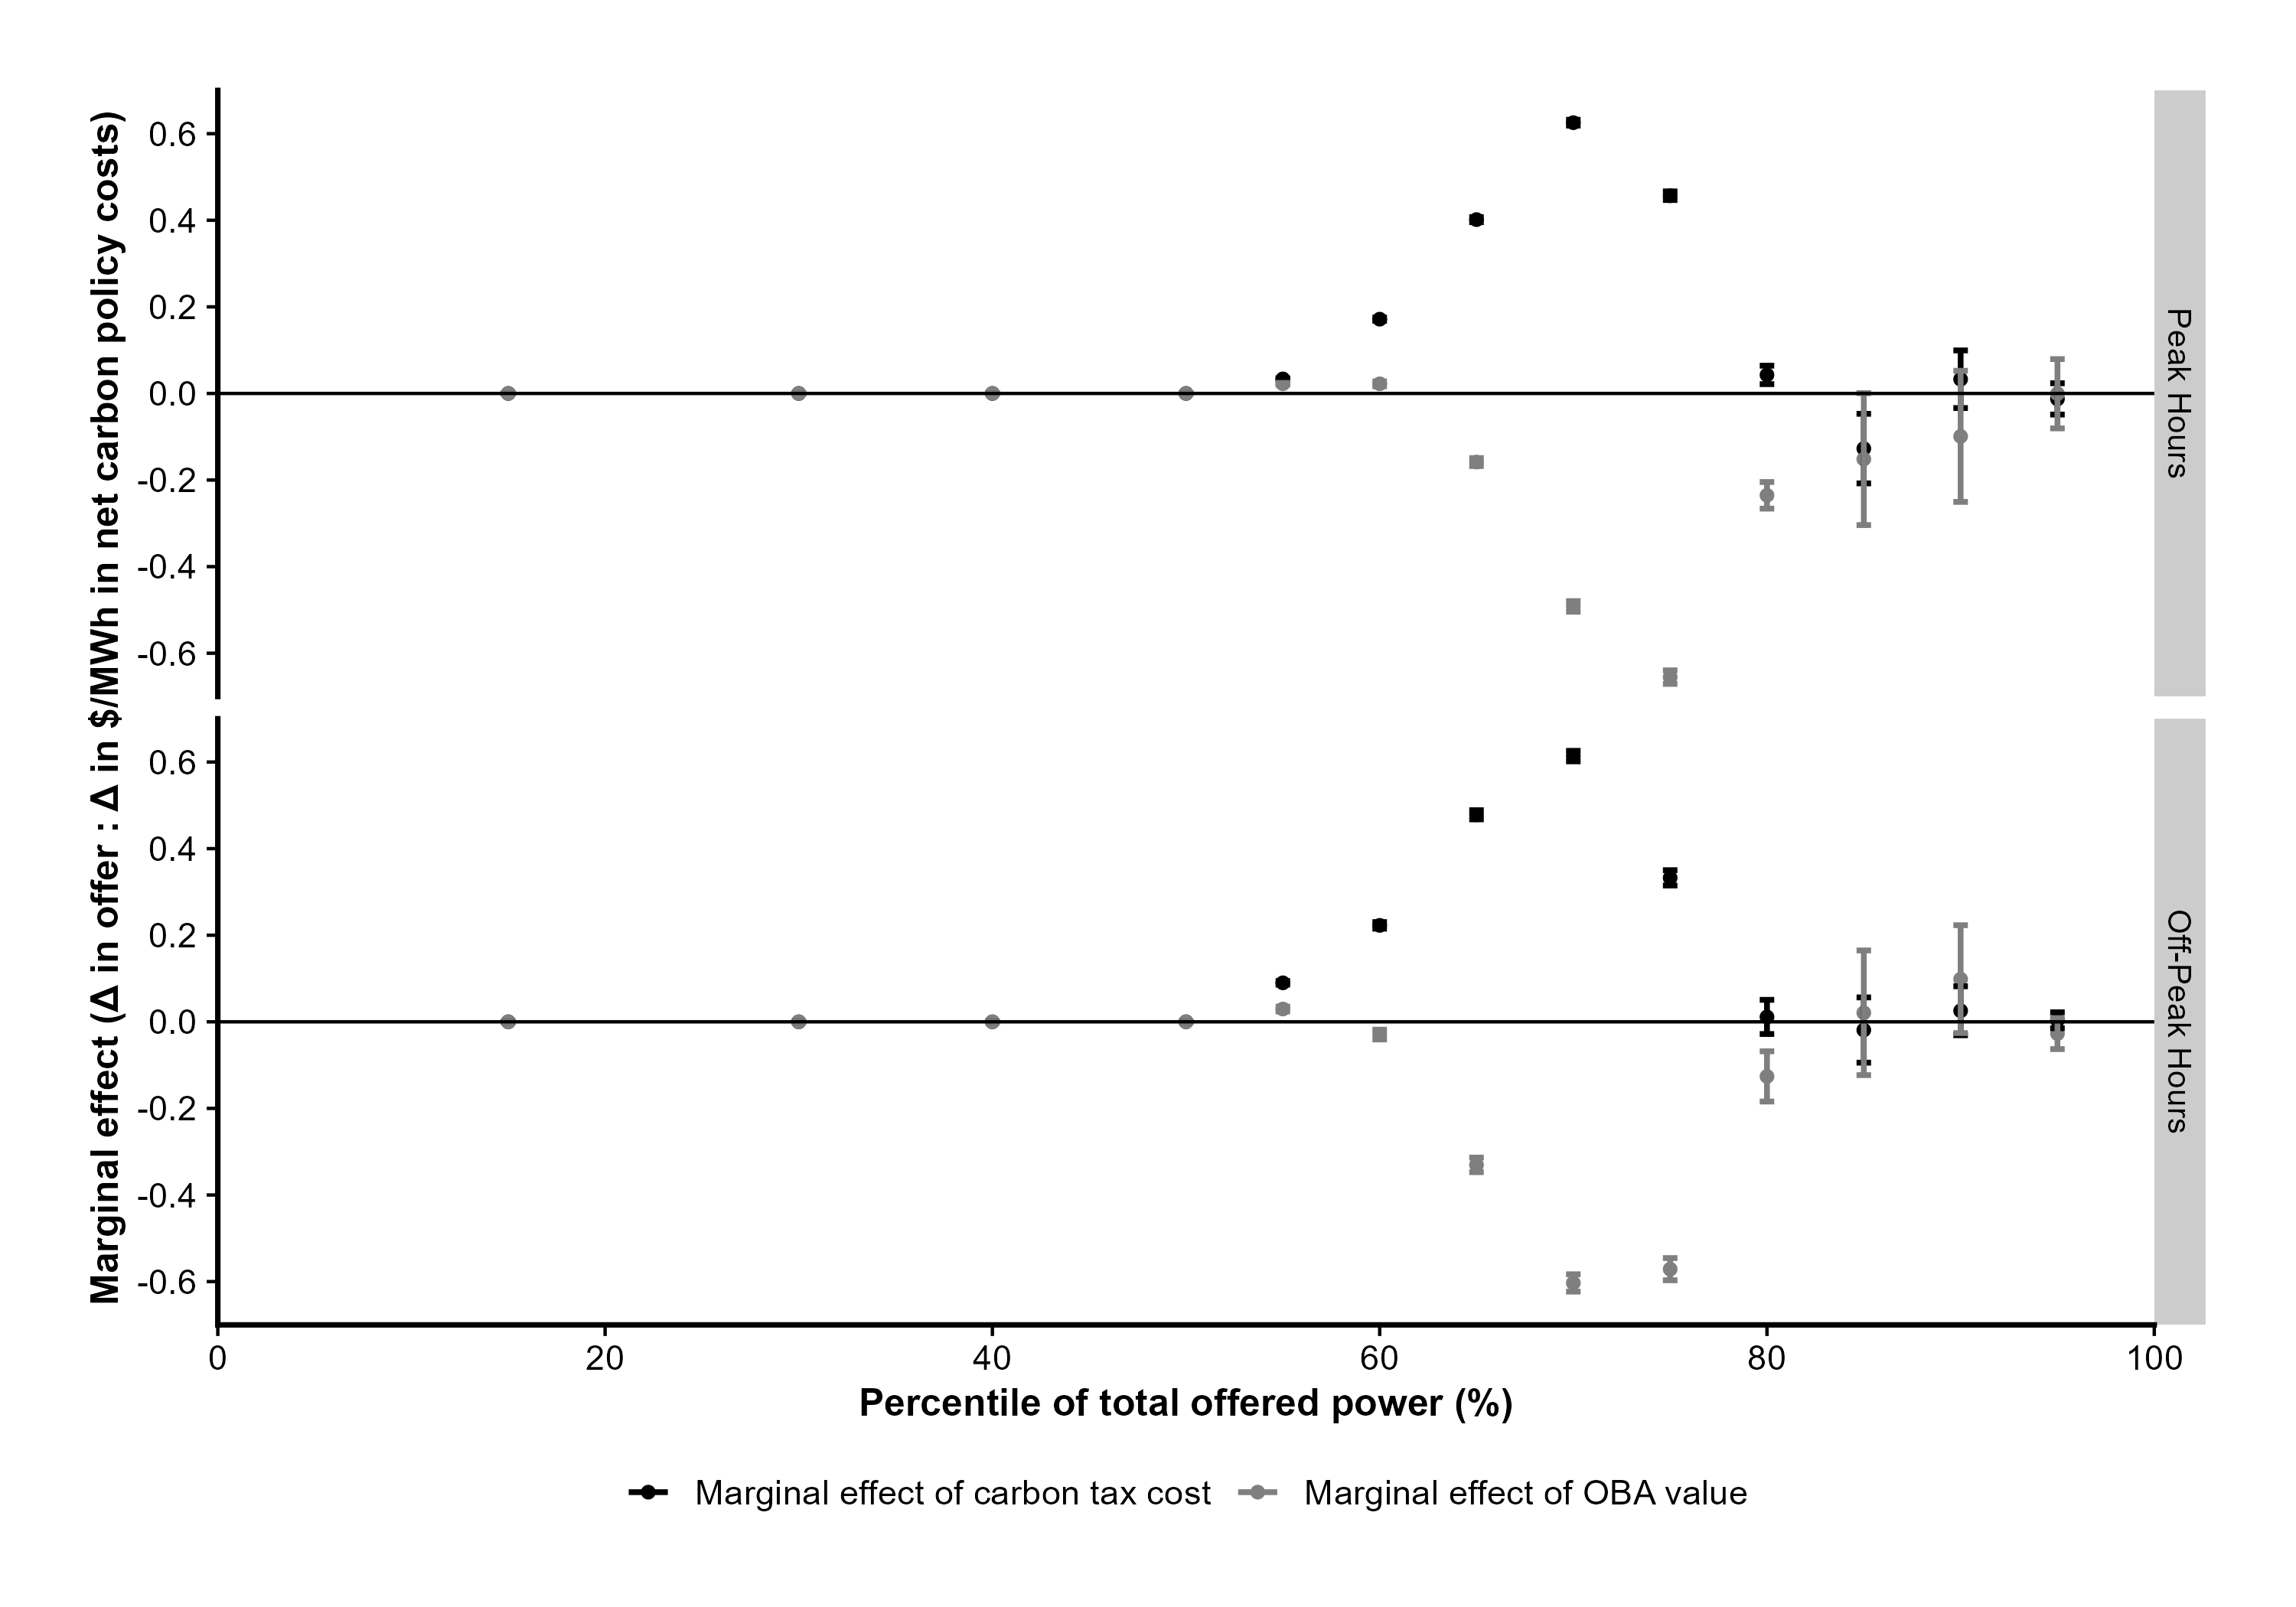
\includegraphics[width=.72\paperwidth]{../images/all_plants_ctax_peak_flex.png}}; \vspace{1cm}
   \vfill
\end{frame}



\begin{frame}{Net impact, all firms, tight vs. slack hours}
   \tikz [remember picture,overlay]
    \node[yshift=-0.52cm,xshift=0cm] at (current page.center)
        {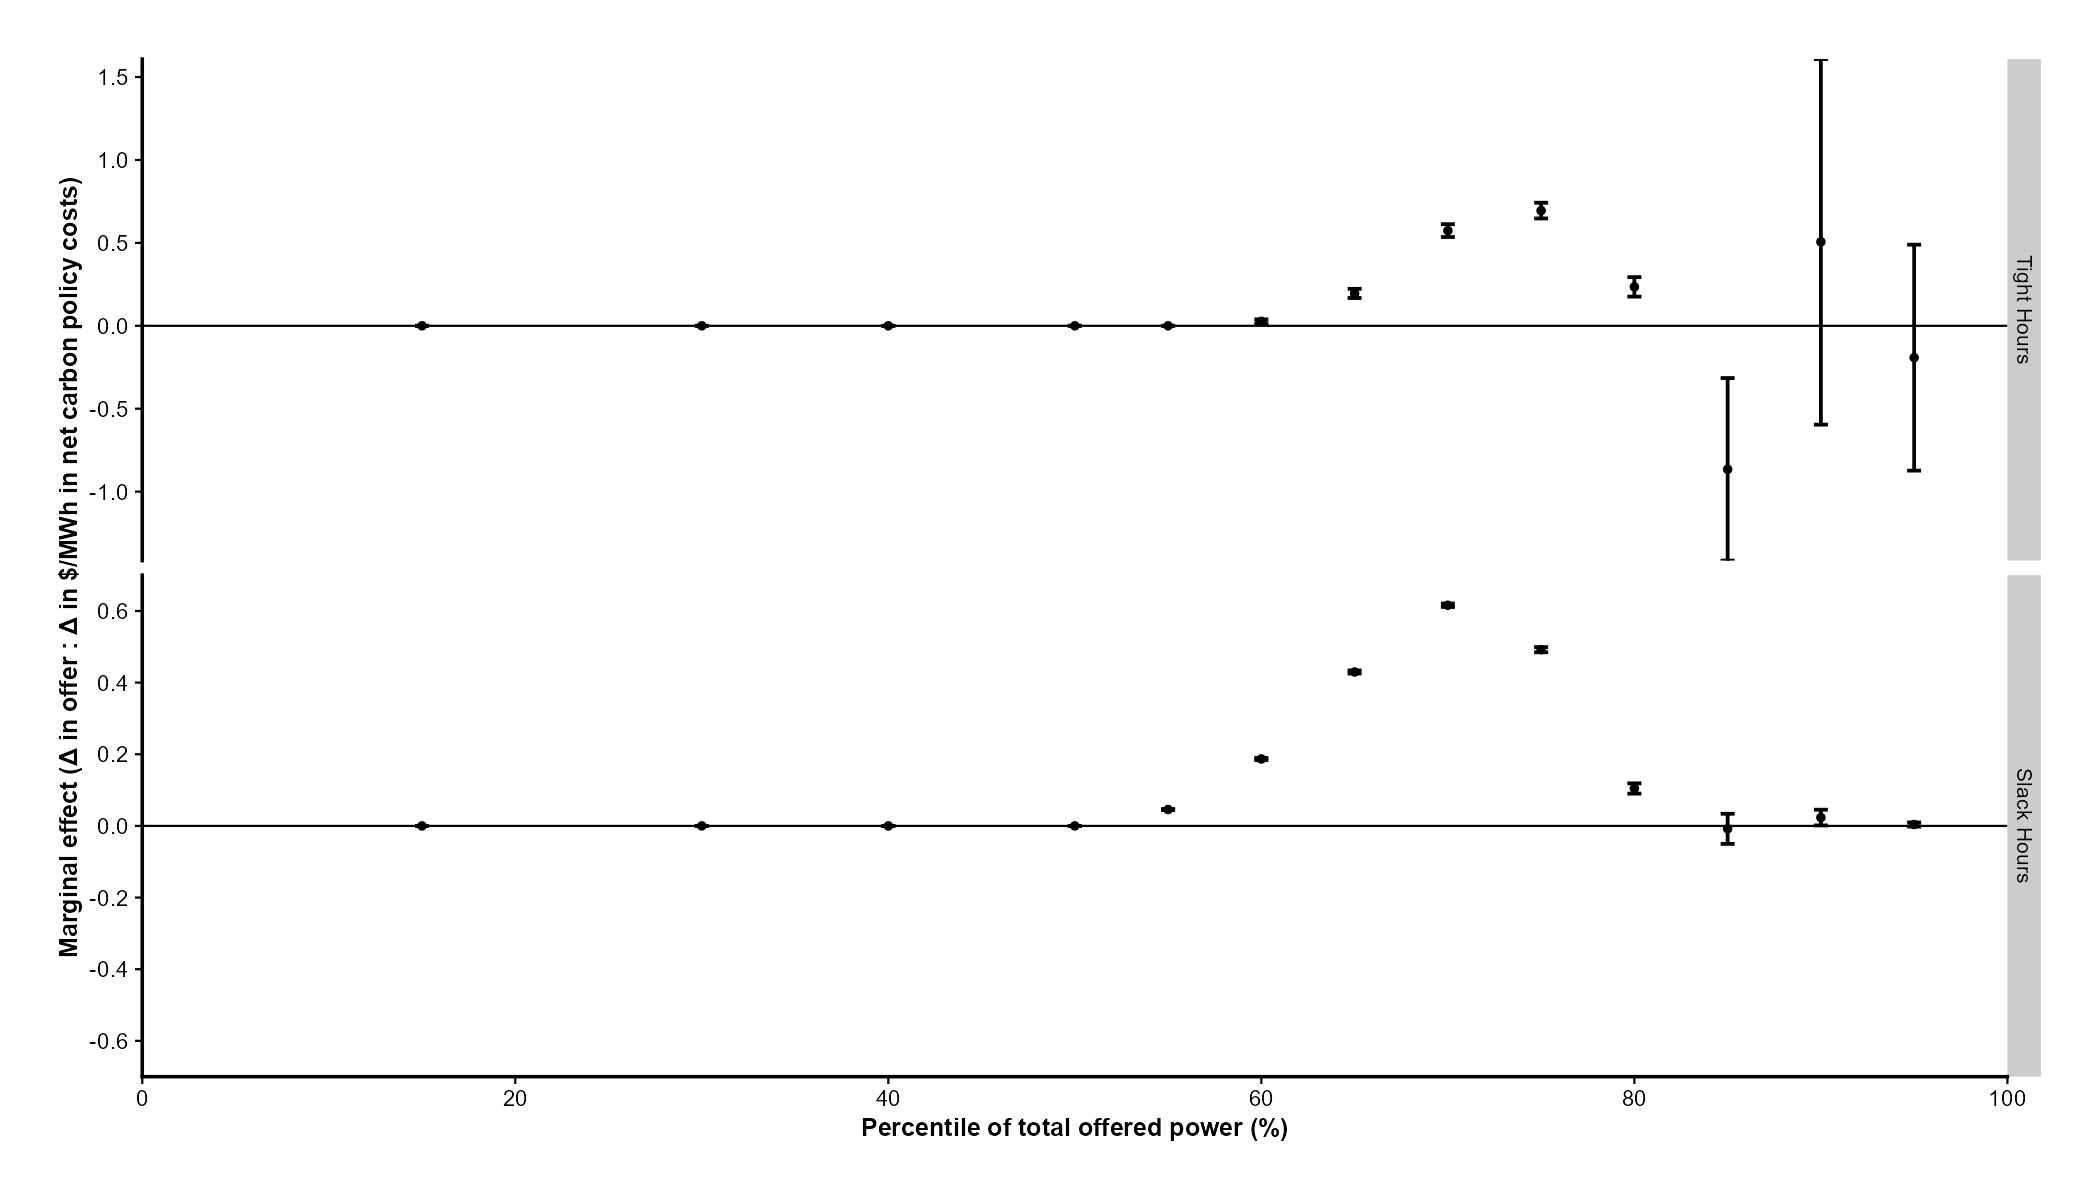
\includegraphics[width=.7\paperwidth]{../images/all_plants_net_tight.png}}; \vspace{1cm}
   \vfill
\end{frame}

\begin{frame}{Coal and Gas Plant Offers}
   \tikz [remember picture,overlay]
    \node[yshift=-0.4cm,xshift=0cm] at (current page.center)
        {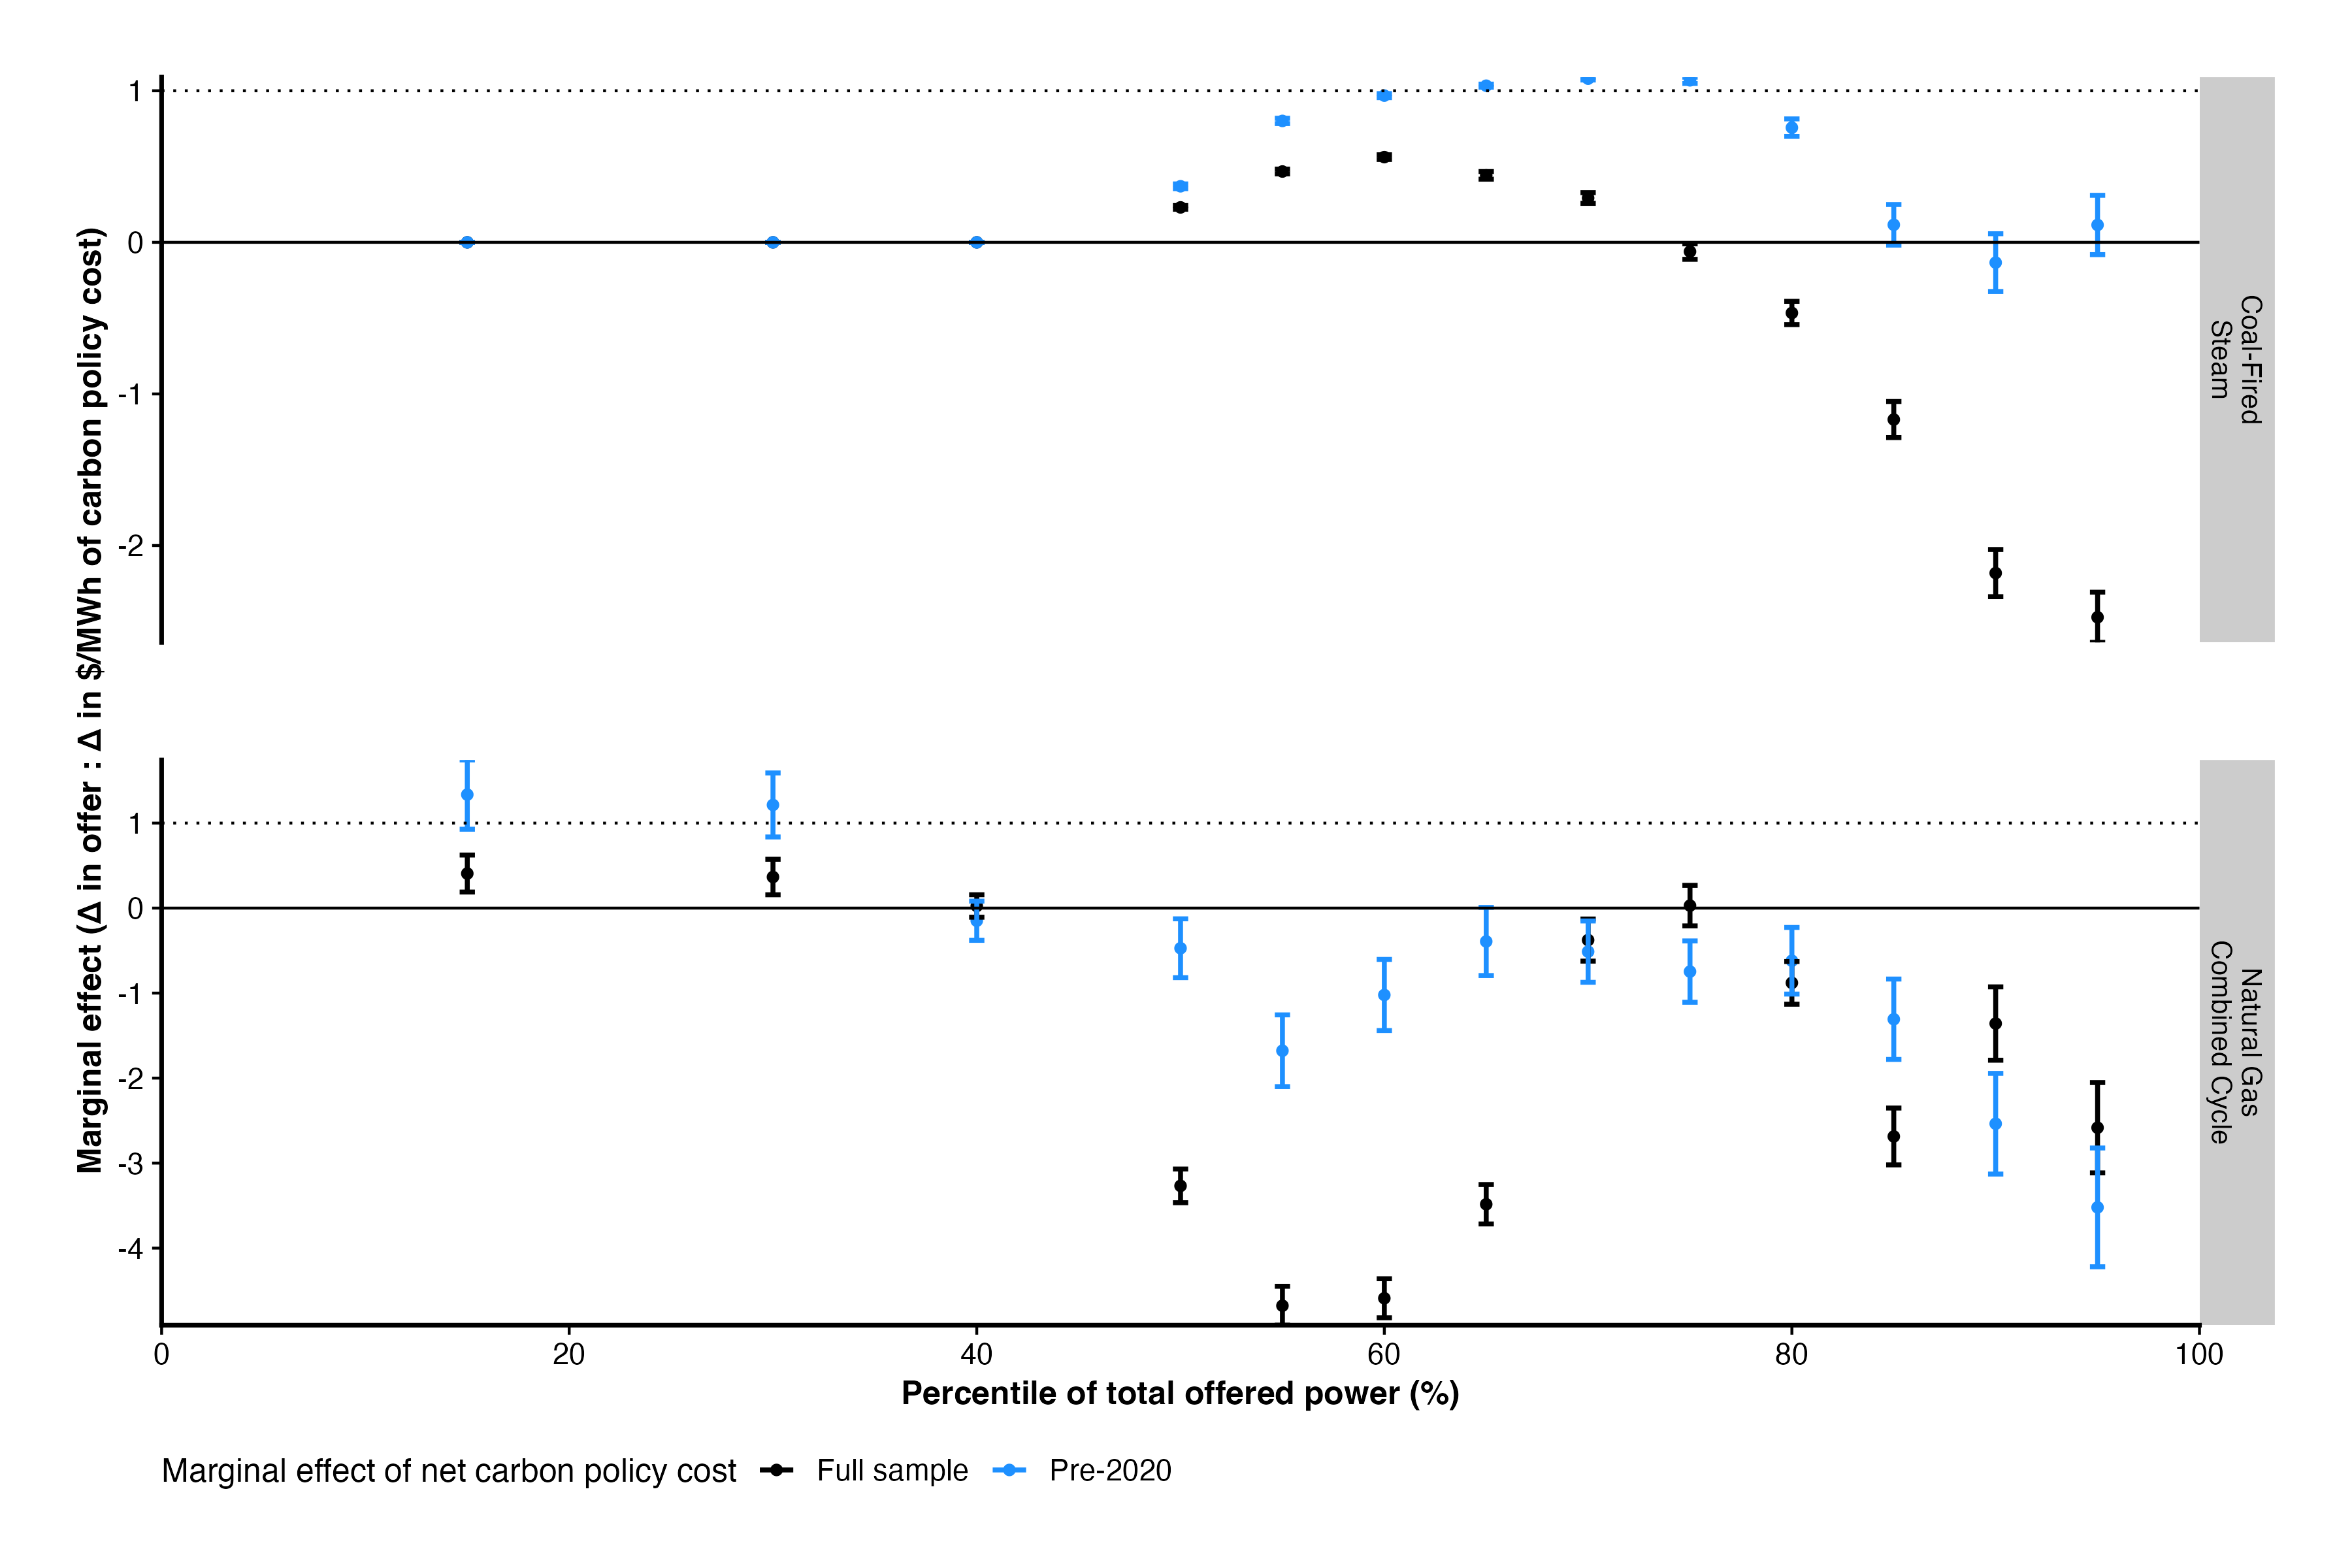
\includegraphics[width=.7\paperwidth]{../images/by_plant_net_talk.png}}; \vspace{1cm}
   \vfill
\end{frame}



\begin{frame}{The Impact of the Balancing Pool Period}
\begin{table}[!h]
\vspace{-0.5cm}
\tiny
\begin{tabular}{lcccccc}
\\[0.5ex]\hline
Facility&Plant&Unit& Capacity& End of& Returned to&Conversion to\\
&Owner&         ID   &  (MW) &  PPA Term &Balancing&gas-fired steam\\
&&                 &    &      & Pool&or retirement\\[+0.5ex]
\hline \\[-1.5ex]
Battle River& ATCO& BR3 &147& Dec 31, 2013&NA&NA\\
&&BR4 &147& Dec 31, 2013&NA&Mar 8, 2022\\
&&BR5 &368& Dec 31, 2020&Jan 1, 2016&Nov 19, 2021\\[+0.75ex]
Genesee &Capital Power &GN1 &381 &Dec 31, 2020&NA&May 1, 2024$^*$\\
&&GN2 &381 &Dec 31, 2020&NA&July 1, 2024$^*$\\
&&GN3 &466 &NA&NA&July 12, 2024$^*$\\[+0.75ex]
HR Milner &ATCO& HRM& 144& Jan 01, 2013&NA&May 8, 2020\\[+0.75ex]
Keephills& TransAlta & KH1 &383& Dec 31, 2020&May 5, 2016&Jan 11, 2022\\
&&KH2& 383& Dec 31, 2020&May 5, 2016&July 21, 2021\\
&&KH3 &466 &NA&NA&Jan 11, 2022$^*$\\[+0.75ex]
Sheerness &ATCO (50\%) & SH1& 378& Dec 31, 2020&Mar 7, 2016&July 30, 2021\\
&TransAlta (50\%)&SH2& 378& Dec 31, 2020&Mar 7, 2016&July 30, 2021\\[+0.75ex]
Sundance A &TransAlta&  SD1 &280& Dec 31, 2020&Mar 7, 2016&Jan 1, 2018$^*$\\
&&SD2 &280& Dec 31, 2020&Mar 7, 2016&July 31, 2018$^*$\\[+0.75ex]
Sundance B &TransAlta & SD3& 353& Dec 31, 2020&Mar 7, 2016&July 31, 2020$^*$\\
&&SD4 &353 &Dec 31, 2020&Mar 7, 2016&Apr 1, 2022$^*$\\[+0.75ex]
Sundance C &TransAlta& SD5& 353& Dec 31, 2020&Mar 24, 2016&Nov 1, 2021$^*$\\
&&SD6& 357& Dec 31, 2020&Mar 7, 2016&Feb 1, 2021\\[+0.75ex]
  \hline
\end{tabular}\\
Note: * denotes a retirement as opposed to a conversion. Supercritical coal units at Keephills (KH3, 466MW, converted to gas Jan 11, 2022) and Genesee (GN3, 466 MW, converted to gas July 12, 2024) were never part of the PPA system, as they were built as merchant generators. A more extensive re-power of the Genesee 1 and 2 units saw them reclassified as natural gas combined-cycle plants after the retirements listed above. 
\end{table}
   \vfill
\end{frame}


\begin{frame}{Hints from the Balancing Pool's offers}
   \tikz [remember picture,overlay]
    \node[yshift=-0.6cm,xshift=0cm] at (current page.center)
        {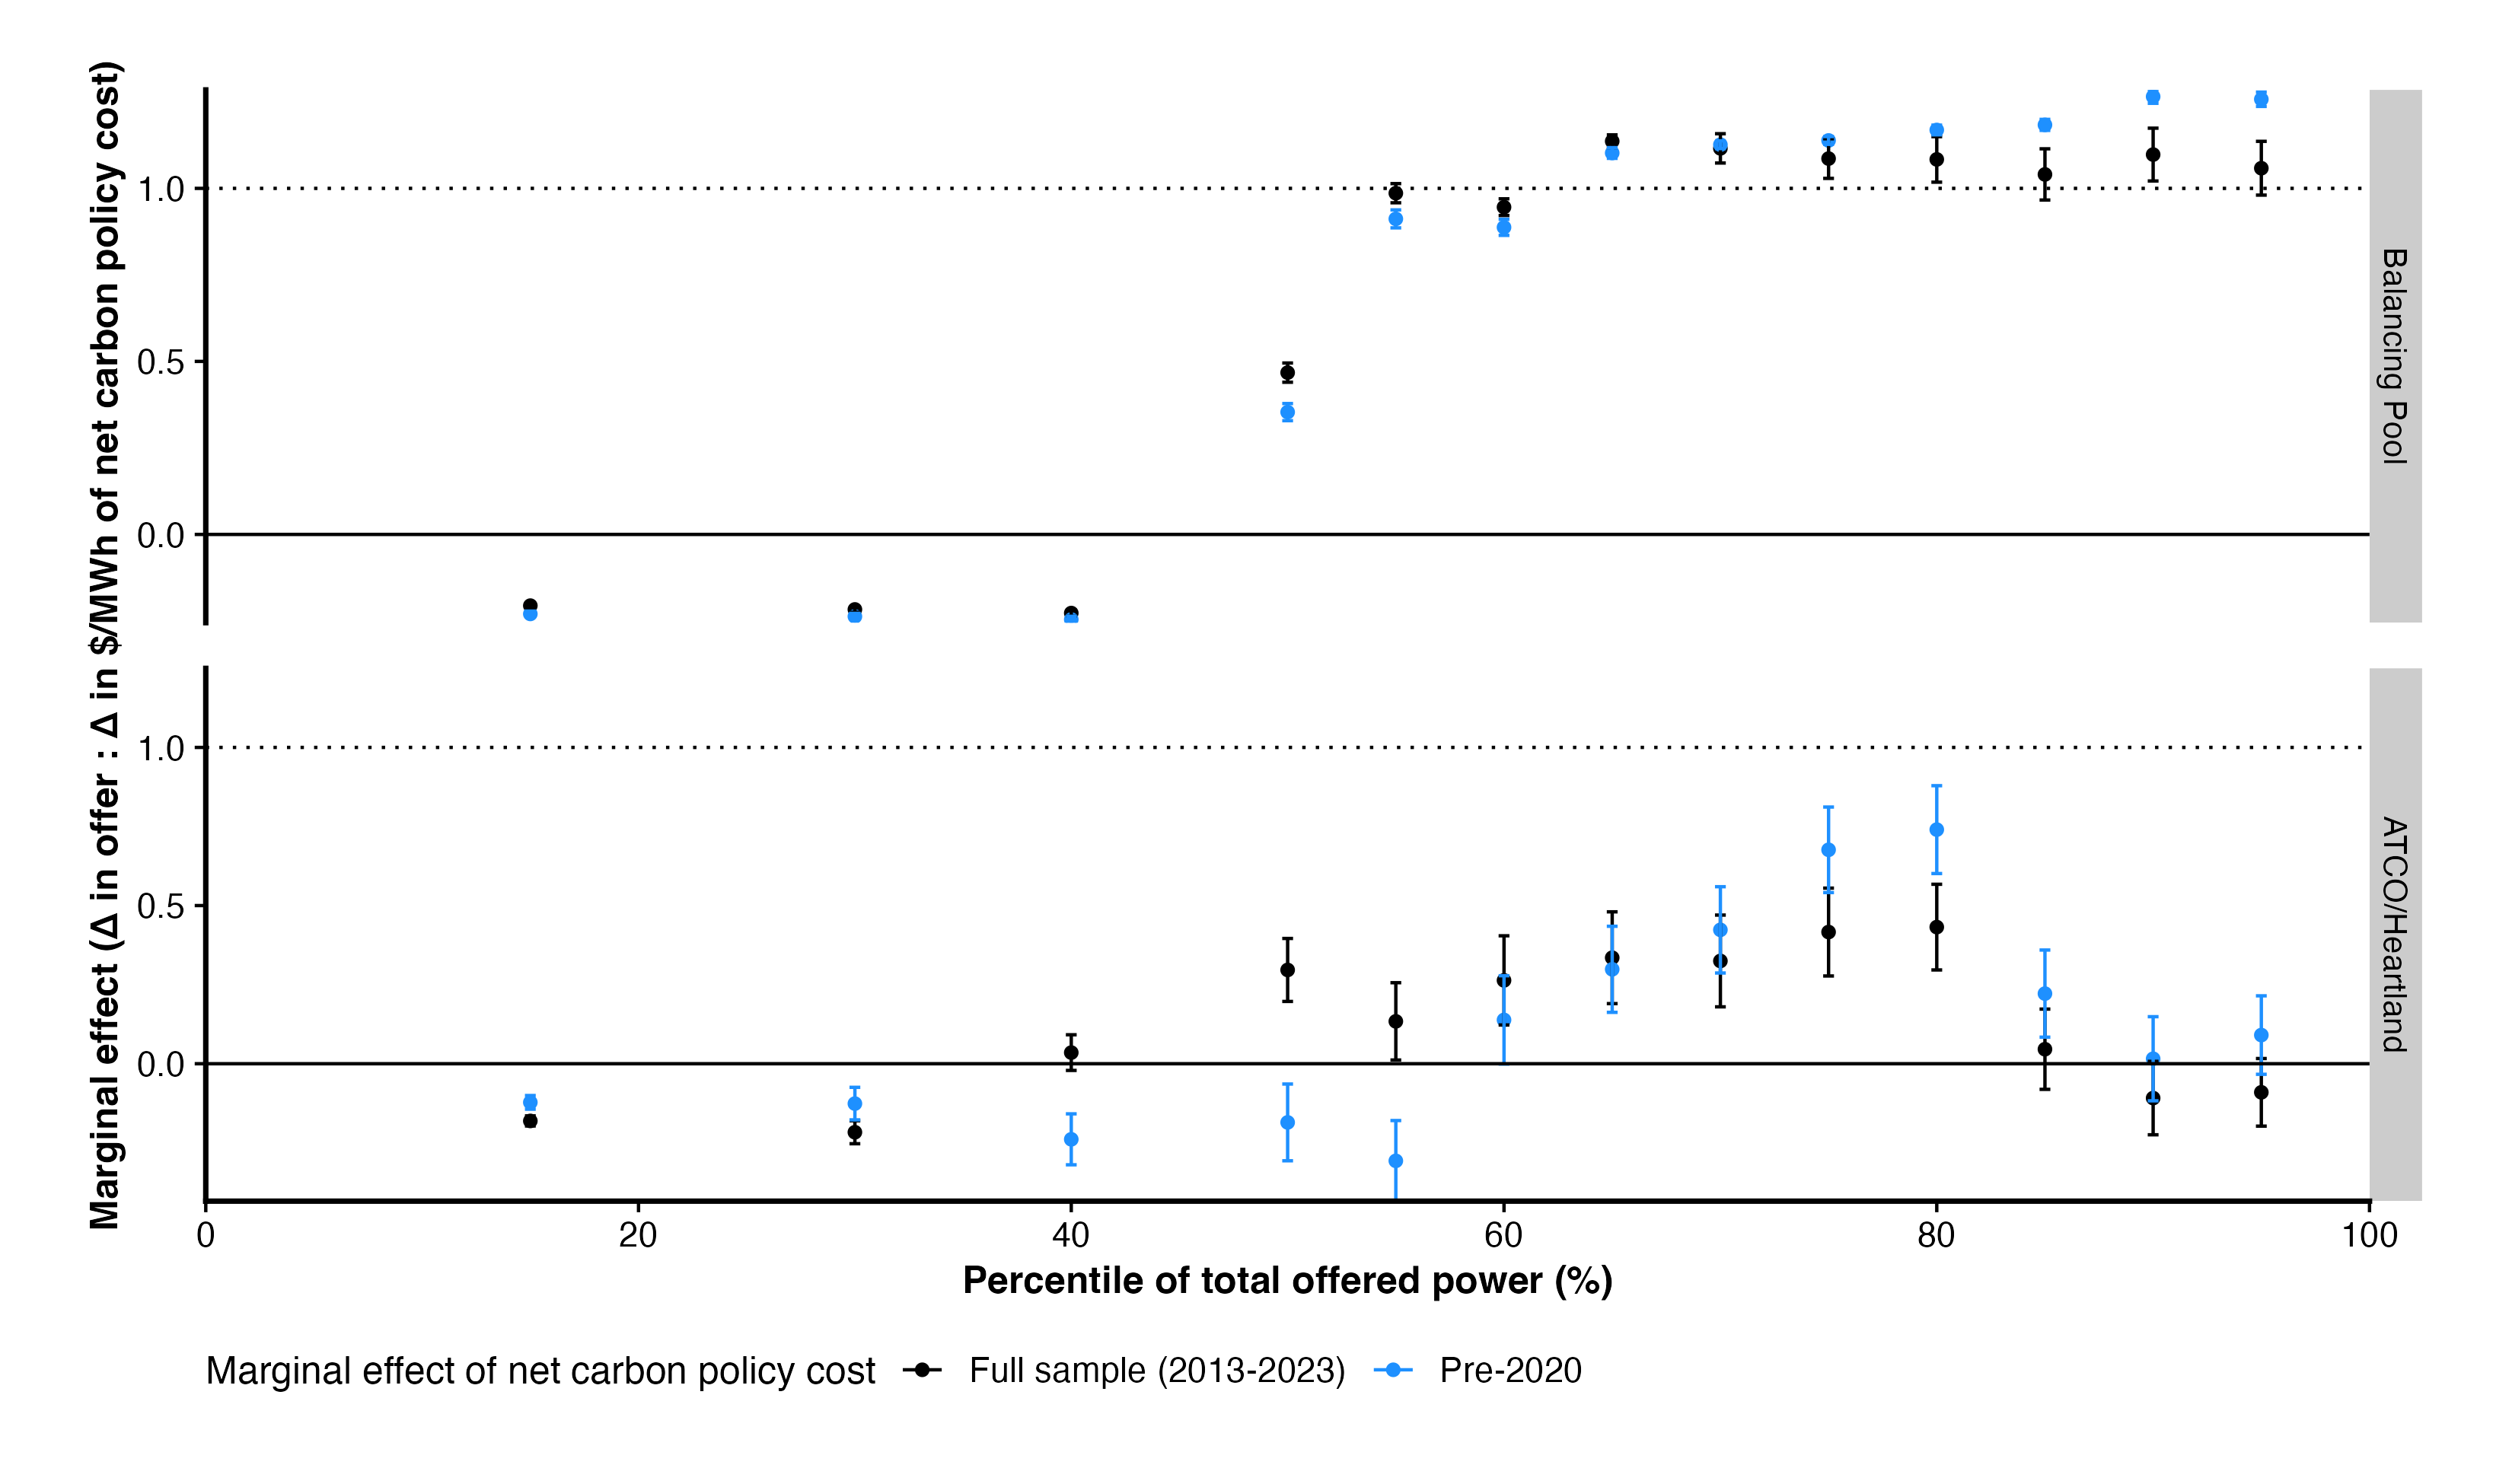
\includegraphics[width=.8\paperwidth]{../images/offers_bp_hl.png}}; \vspace{1cm}
   \vfill
\end{frame}


\section{Discussion}

\begin{frame}{Discussion}
   \begin{itemize}
   \item Alberta's energy-only power market provides an ideal environment to study carbon price pass-through
   \item Results provide no support for full-cost pass-through in any hours
    \item Results suggest that strategic considerations are overwhelming carbon price pass-through incentives
    \item What's missing from the empirical work: ML estimates with right and left censoring of true opportunity costs of power
    \item Confounding factors I'm not sure we can deal with despite the wealth of data
    \item Questions for additional research
    \end{itemize}
   \vfill
\end{frame}


\begin{frame}{Contact info}
\begin{center}
Andrew Leach\bigskip \\
Department of Economics and Faculty of Law, University of Alberta\bigskip \\
Email: \href{mailto:aleach@ualberta.ca}{andrew.leach@ualberta.ca}\bigskip \\
Twitter / X: \href{http://x.com/andrew_leach}{\url{@andrew_leach}}
\end{center}
\vfill
\end{frame}


\end{document} 